\documentclass[11pt,a4paper,twoside]{book}

% LaTeX-Umsetzung der "Richtlinien für Projekt- und Diplomarbeiten"
% der LFE Medieninformatik, LMU München. (Autor: Richard Atterer, 27.9.2006, 23.10.2007), Bug-Fixing Mark Kaczkowski (23.6.2008)

\usepackage[T1]{fontenc} % sonst geht \hyphenation nicht mit Umlauten
%\usepackage[latin1]{inputenc} % man kann schreiben äöüß, statt "a"o"u"s
\usepackage[utf8]{inputenc} % wie oben, aber UTF-8 als Encoding statt ISO-8859-1 (latin1)
\usepackage[ngerman]{babel} % deutsche Trennregeln, "Inhaltsverzeichnis" etc.
%\usepackage{ngerman} % Alternative zum Babel-Paket oben
\usepackage{mathptmx} % Times-Roman-Schrift (auch für mathematische Formeln)
\usepackage{listings} % Für Codefragmente
\usepackage{amsmath}
\usepackage[round]{natbib}
\usepackage[toctitles]{titlesec} % unterschiedlich lange Titel in Kopfzeile und Inhaltsverzeichnis

% Zum Setzen von URLs
\usepackage{color}
\definecolor{darkred}{rgb}{.25,0,0}
\definecolor{darkgreen}{rgb}{0,.2,0}
\definecolor{darkmagenta}{rgb}{.2,0,.2}
\definecolor{darkcyan}{rgb}{0,.15,.15}
\usepackage[plainpages=false,bookmarks=true,bookmarksopen=true,colorlinks=true,
  linkcolor=darkred,citecolor=darkgreen,filecolor=darkmagenta,
  menucolor=darkred,urlcolor=darkcyan]{hyperref}

% pdflatex: Bilder in den Formaten .jpeg, .png und .pdf
% latex: Bilder im .eps-Format
\usepackage{graphicx}
\usepackage{multirow}
\usepackage{pdfpages}

\usepackage{ifthen,hyperref}
\usepackage[german,vario]{fancyref}
\definecolor{darkblue}{rgb}{0,0,.5}
\hypersetup{colorlinks=true, breaklinks=true, linkcolor=darkblue, menucolor=darkblue, urlcolor=darkblue, citecolor=darkblue}

%----------------------------------------------------------
\renewcommand*{\fancyrefdefaultspacing}{%
\fancyreftightspacing
}

\makeatletter

\let\@f@ref@sav=\@f@ref
\renewcommand*{\@f@ref}[4]{%
\def\@curtlabtype{#3}%
\protect\@f@ref@sav{#1}{#2}{#3}{#4}%
}%
\addto\extrasngerman{%
\renewcommand\reftextfaraway[1]{%
\ifthenelse{\equal{\@curtlabtype}{chap}}{ab Seite}{%
\ifthenelse{\equal{\@curtlabtype}{sec}}{ab Seite}{auf Seite}}~\pageref{#1}}
}

\makeatother
%----------------------------------------------------------

\usepackage{fancyhdr} % Positionierung der Seitenzahlen
\fancyhead[LE,RO,LO,RE]{}
\fancyfoot[CE,CO,RE,LO]{}
%\fancyfoot[LE,RO]{\Roman{page}}
\renewcommand{\headrulewidth}{0pt}
\setlength{\headheight}{13.6pt} % behebt headheight Warning

% Absatz Einruecken und Space
\setlength{\parindent}{0pt}
\setlength{\parskip}{\baselineskip}

% Korrektes Format für Nummerierung von Abbildungen (figure) und
% Tabellen (table): <Kapitelnummer>.<Abbildungsnummer>
\makeatletter
\@addtoreset{figure}{section}
\renewcommand{\thefigure}{\thesection.\arabic{figure}}
\@addtoreset{table}{section}
\renewcommand{\thetable}{\thesection.\arabic{table}}
\makeatother

\sloppy % Damit LaTeX nicht so viel über "overfull hbox" u.Ä. meckert

% Ränder
\addtolength{\topmargin}{-16mm}
\setlength{\oddsidemargin}{25mm}
\setlength{\evensidemargin}{35mm}
\addtolength{\oddsidemargin}{-1in}
\addtolength{\evensidemargin}{-1in}
\setlength{\textwidth}{15cm}
\addtolength{\textheight}{34mm}

\begin{document}

\pagestyle{empty} % Vorerst keine Seitenzahlen
\pagenumbering{arabic} % Unsichtbare alphabetische Nummerierung

\begin{center}
\textsc{Ludwig-Maximilians-Universität München}\\
Institut für Informatik\\
Lehrstuhl für Mensch-Maschine-Interaktion\\
Prof.\ Dr.\ Andreas Butz

\vspace{5cm}
{\large\textbf{Masterarbeit}}\vspace{.5cm}

{\LARGE Modelling Multimodal Interaction in the Car}\vspace{1cm}

{\large Carina Rothe}\\\href{carina.saliger@live.de}{carina.saliger@live.de}

\end{center}
\vfill

\begin{tabular}{ll}
Bearbeitungszeitraum: & 16. 09. 2016 bis 17. 03. 2017\\
Betreuer: & Dr.\ Bastian Pfleging \\
Externer Betreuer von BMW: & Dipl. Ing. Florian Roider\\
Verantw. Hochschullehrer: & Prof. Dr.\ Butz 
\end{tabular}
\cleardoublepage
\chapter*{Zusammenfassung}
Informationssysteme im Auto werden immer komplexer und werden teils schon mit multimodalen Eingaben wie Sprache, Touch oder Gestik bedient.
Diese multimodalen Interaktionen eröffnen den Nutzern neue Möglichkeiten, die passende Modalität je nach Situation und Eignung zu wählen.
Allerdings muss darauf geachtet werden, die Ablenkung des Fahrers gering zu halten und die Modalitäten in geeigneten Kombinationen zu unterstützen.

Dadurch motiviert erstellen wir in dieser Arbeit ein multimodales Modell, dass Designern multimodaler Schnittstellen helfen soll, die Interaktionszeiten verschiedener Modalitäten vorherzusagen und zu vergleichen.
Dazu entwickeln wir einen Prototypen, der mit Touch, Geste und Sprache bedient werden kann.
Mittels eines within-subject Design testen 22 Probanden in vier Anwendungsbeispielen alle Kombinationen von Modalitäten mit einem Moduswechsel, sowie die entsprechenden unimodalen Varianten.
Aus diesen Interaktionszeiten leiten wir ein Modell mit verschiedenen Aktionszeiten für die Modalitäten Touch, Sprache und Geste ab, sowie deren Wechselkosten untereinander.
Unser Modell lehnt sich an das Konzept des Keystroke-Level Modells und Erweiterungen an.
Wir konzentrieren uns jedoch nicht auf einzelne Operatoren, sondern auf grob körnigere Aktionen und deren Wechselkosten.

Zur Validierung des multimodalen Modells werden in einer weiteren Studie fünf verschiedene Aufgaben mit bis zu vier Moduswechseln untersucht und mit unserer Vorhersage des Modells verglichen.
Es zeigte sich, dass unser Modell multimodale Interaktionen mit einem durchschnittlichen Vorhersagefehler von 14,746\% vorhersagen konnte
Diese Abschätzung von multimodalen Interaktionszeiten im Auto ermöglicht es Designern bereits in einem frühen Stadium der Entwicklung zu unterstützen und hilft ihnen die Ablenkung des Fahrers zu minimieren.


%\selectlanguage{english}
\chapter*{Abstract}
In-Vehicle-Information-Systems are getting more and more complex and the possibilities for using multimodal interactions like speech, touch and gestures are growing.
A big advantage of multimodal interactions is that a user can decide in which situation he wants to use the most suitable kind of interaction.
ON the other hand such a multimodal system should minimize the distraction of the driver and support the best combinations of modalities.

Motivated by this we design in this thesis a multimodal model to support designers of multimodal interfaces by predicting the interaction time of such systems.
By comparing interaction times, the best combinations can be detected and a favorable design is possible.
Our model is similar to the concept of the keystroke-level-model and its extensions.
However we focus on actions for each modality and the resulting change costs instead of single operators.
With the measured interaction times of our first study we develope a model with different times for each modality (touch, speech and gestures).
We also model the changing costs between one modality to another.

To validate our multimodal model we investigate in a second study five tasks and compared the total task time with the prediction time of our model.
We show that the prediction time of our model is a good match compared to the observed times.
The average RMSE was 14,746\%.
These predictions can support designer in an early stage of implementation and help them to reduce driver distraction.

%\selectlanguage{ngerman}
\clearpage
\chapter*{Aufgabenstellung}
In modernen Autos wird die Funktionalität von Informationssystemen im Auto immer komplexer. Es ist wichtig dem Nutzer eine einfache Eingabe zu ermöglichen, ohne ihn zu sehr visuell oder mental zu belasten. Durch die steigende Anzahl an eingebauter Technik in Autos wachsen auch die Eingabemöglichkeiten des Fahrers. Das Infotainmentsystem (IVIS) kann nicht nur durch haptische Knöpfe und Schalter oder Touch bedient werden, sondern auch per Sprache, Gesten und Blick. Die meisten Eingabeoptionen sind schon in aktuelle Autos integriert, jedoch ist es schwer für Entwickler der Schnittstellen, die Benutzbarkeit aller Eingabeoptionen sowie deren Kombination einzuschätzen, zum Beispiel bzgl. der Aufgabendauer.

Im Zuge dieser Masterarbeit soll daher die Bedienung im Fahrzeug beobachtet werden mit dem Ziel, die multimodale Interaktion für künftige Systeme modellieren zu können. Ein Beispiel dazu ist eine Erweiterung des Keystroke-Level Modells auf Bedienaufgaben eines multimodalen IVIS mit verschiedenen Inputmodalitäten, um damit Bedienzeiten vorhersagen zu können. Primäre Aufgabe wird dabei die Analyse und Berechnung von Interaktionszeiten. Dies erfordert einerseits eine aktuelle Bestandsaufnahme bzgl. existierender Modelle wie zum Beispiel erweiterten KLMs und deren Operatoren. Neue Bedienmöglichkeiten erfordern zudem die Ermittlung neuer Operatoren, um die Interaktion mit heutigen IVIS (zum Beispiel per Touch, Sprache und Geste) darstellen zu können. Ein besonderer Aspekt ist dabei die multimodale Bedienung, bei der zum Beispiel Handlungen nacheinander oder alternativ über verschiedene Modalitäten abgewickelt werden, die dementsprechend unterschiedlich lang dauern können (auch: Wechselzeiten / -kosten).

Basierend auf den empirisch zu ermittelnden Operatoren und Operatorzeiten soll dann ein erweitertes Modell erstellt werden, das die Vorhersage für eine multimodale Interaktion im Fahrzeug ermöglicht. Ein solches Modell kann dazu dienen, verschiedene Interaktionsmöglichkeiten zu vergleichen und erlaubt insbesondere in frühen Designphasen eine schnelle Abschätzung bzgl. der Interaktionsdauer im Fahrzeug.

Zu diesem Zweck ist es sowohl unter den Aspekten der Bedienbarkeit, der User Experience also auch der Fahrsicherheit / Fahrerablenkung geplant, verschiedene Untersuchungen (zum Beispiel Umfragen, Fokusgruppen, Laborstudien) durchzuführen, um Operatoren und Interaktionszeiten zu messen und zu validieren. Im Speziellen sind die folgenden Schritte angedacht:

\begin{enumerate}
\item Recherche: Finden verwandter Arbeiten und Analyse des aktuellen Stands von IVIS \& KLM 
\item Evtl. Nutzerbefragung/Brainstorming-Runde, um herauszufinden, welche Gesten und Sprachbefehle auf die Anwendungsbeispiele von Touch am besten geeignet sind. 
\item Planung und Durchführung einer Studie zur Bestimmung von Interaktionszeiten multimodaler Interaktion im Fahrzeug. 
\item Ableitung eines geeigneten Modells. 
\item Validierung des Modells in einer weiteren Studie. 
\item Ggfs. Gestaltung eines Tools zur vereinfachten Berechnung von Interaktionen für neue Prototypen 
\end{enumerate}

\vfill % Sorgt dafür, dass das Folgende an das Seitenende rutscht

\noindent Ich erkläre hiermit, dass ich die vorliegende Arbeit
selbstständig angefertigt, alle Zitate als solche kenntlich gemacht
sowie alle benutzten Quellen und Hilfsmittel angegeben habe.

\bigskip\noindent München, \today

\vspace{4ex}\noindent\makebox[7cm]{\dotfill}

\cleardoublepage
\pagestyle{fancy}
%\pagenumbering{roman} % Römische Seitenzahlen
%\setcounter{page}{1}

% Inhaltsverzeichnis erzeugen
\setlength{\parskip}{1pt}
\tableofcontents
\setlength{\parskip}{\baselineskip}

%Abbildungsverzeichnis erzeugen - normalerweise nicht nötig
%\cleardoublepage
%\listoffigures

\cleardoublepage

% Arabische Seitenzahlen
%\pagenumbering{arabic}
%\setcounter{page}{1}
% Geändertes Format für Seitenränder, arabische Seitenzahlen
\fancyhead[LE,RO]{\rightmark}
\fancyhead[LO,RE]{\leftmark}
\fancyfoot[LE,RO]{\thepage}

\chapter{Einleitung}
Schon längst besteht Autofahren aus mehr als lediglich dem Bedürfnis, von A nach B zu kommen.
Ein Fahrer will im Auto vielmehr auch die Möglichkeit haben Dinge zu nutzen, welche nichts mit der Hauptaufgabe des Fahrens (Primäre Aufgabe) zu tun haben.
Zum Beispiel navigiert sich der Autofahrer zu seinem Ziel, hört Musik, findet die nächste Tankstelle in der Umgebung, nimmt ein Telefongespräch an, sowie vieles mehr.
Somit werden in aktuellen Autos die Funktionalität von Informationssystemen im Auto (IVIS von "`In-Vehicle-Information System"') komplexer und die Inhalte umfangreicher \citep{Kern:2009}.
Hierbei besteht die Aufgabe und Herausforderung für Designer diese Masse an Information in geeigneter Weise für den Fahrer darzustellen und nutzbar zu machen.
Dauert eine Interaktion mit einem IVIS zu lange oder ist sie schwer zu verstehen, sind dies häufig Gründe für zu große Ablenkungen beim Fahren, was Autounfälle mit sich zieht \citep{neale2005overview}.
Daher sollten diese potenziellen Ablenkungen so minimal wie möglich gehalten werden.
Zusätzlich ist es wichtig, dem Nutzer eine einfache und intuitive Eingabe des Informationssystems im Auto zu ermöglichen, ohne ihn gleichzeitig zu sehr visuell oder mental zu belasten. 

Hinzu kommt, dass die Bedienung von jeglichen Funktionen im Auto längst nicht mehr unimodal sind.
Unimodal bezeichnet hierbei die Interaktion zwischen Mensch und Auto, welche lediglich eine Modalität verwendet, wie zum Beispiel haptische Bedienelemente.
Dagegen ist es dem Fahrer möglich verschiedenste Funktionen multimodal auszuführen.
Zu den üblichen haptischen Bedienelementen kommen somit zusätzlich Touchdisplays oder Möglichkeiten der Sprachbedienung, die in Kombination betätigt werden können. 
 
Eine weit verbreitete Modalität ist die Spracheingabe, die zum Beispiel oft genutzt wird, um ein Telefonanruf zu starten oder anzunehmen. Dazu wird meist ein haptischer "`Push to Talk"' Button gedrückt und anschließend der Sprachbefehl gesagt. 

Ein wesentlicher Vorteil der Sprachsteuerung ist, dass die Hand nicht vom Lenkrad genommen werden muss und auch der Blick auf der Straße verbleiben kann.
\citet{maciej2009comparison} sind der Überzeugung, dass Sprachbedienung eine Unerlässlichkeit in zukünftigen Autos sein wird.
Allerdings ist bei einer Autofahrt mit mehreren Mitfahrern, bei der geredet und Musik gehört wird, die Sprachsteuerung nicht immer optimal. 

Auch Gestensteuerungen sind in einigen Autos bereits vertreten.
Zum Beispiel wird im BMW 7er eine Kreisbewegung mit dem Finger nach rechts bzw. links erkannt, um die Lautstärke zu erhöhen beziehungsweise zu verringern. 
Es ist allerdings meist nicht möglich mit einer dieser neuen Modalitäten alle vorhandenen Funktionen auszuführen.
Ein Interface heißt seriell-redundant, wenn Modalitäten wie zum Beispiel Sprache, Gestik oder Touch beliebig gewechselt werden können \citep{neuss_2001}. 

Mit einem seriell-redundanten multimodalen Informationssystemen im Auto könnte der Fahrer selbst entscheiden in welchen Situationen welcher Modus für den jeweiligen Schritt am einfachsten und sichersten ist.
Dies stellt nach \citet{Muller_2011} einen wesentlichen Vorteil im Auto dar.
Natürlich gibt es auch Kombinationen, welche mit bestimmten Modalitäten weniger sinnvoll sind als andere.
Unsere Motivation ist deshalb, solche multimodalen Interaktionen in IVIS zukünftig besser zu verstehen, um diese optimal umsetzen zu können.
Es ist wichtig die schnellsten und einfachsten Kombinationen verschiedener Modalitäten zu kennen, um dem Fahrer auch die besten Möglichkeiten in verständlicher Weise anzuzeigen.
Damit soll die visuelle und mentale Beanspruchung für den Fahrer so gering wie möglich gehalten werden. 

Um Interfaces bereits in einem frühen Stadium der Entwicklung zu testen wurde in der Vergangenheit häufig das Keystroke-Level Modell in der ursprünglichen oder den erweiterten Varianten verwendet.
Damit können bereits vor der Implementierung eines Prototyps Interfacekonzepte auf ihre Bediendauer getestet werden, indem die Dauer einer gewählten Aufgabe vorhergesagt wird.
Somit wird es möglich, auf einfache Art verschiedene Varianten zu vergleichen.
Das Keystroke-Level Modell bezieht sich in der ursprünglichen Variante nur auf Desktop-basierte Anwendungen, die sich hauptsächlich auf Textverarbeitungsprogramme bezogen.
In den letzten Jahrzehnten wurde dieses vereinfachte Konzept jedoch auch auf Geräte und Anwendungen übertragen und erwies sich hierbei als geeignete Methode zur Einschätzung der Interaktionsdauer. 

Das Ziel dieser Arbeit ist es, dieses Konzept für seriell redundante multimodale IVIS zu adaptieren und anzupassen.
Dazu entwickeln wir ein Modell, mit dem Interaktionszeiten eines multimodalen IVIS vorhergesagt und verglichen werden können.
Wir konzentrieren uns auf die Modalitäten Touch, Sprache und Geste und auf die entstehenden Kosten bei einem Wechsel zwischen zwei Modalitäten.
Jede Modalität besitzt ihre Vorteile und Nachteile und kann in geeigneter Kombination den Fahrer optimal unterstützen.

Im Zuge dieser Masterarbeit soll daher die Bedienung im Fahrzeug beobachtet werden, mit dem Ziel die multimodale Interaktion für künftige Systeme modellieren zu können.
Ein besonderer Aspekt liegt dabei auf der multimodalen Bedienung, bei der zum Beispiel Handlungen nacheinander oder alternativ über verschiedene Modalitäten abgewickelt werden.
Die Aktionen können dementsprechend unterschiedlich lang dauern und Wechselkosten enthalten.
Basierend auf den empirisch zu ermittelnden Operatoren und Operatorzeiten soll dann ein erweitertes Modell erstellt werden, welches die Vorhersage für eine multimodale Interaktion im Fahrzeug ermöglicht.
Zu diesem Zweck ist es sowohl unter den Aspekten der Bedienbarkeit und User Experience, als auch der Fahrsicherheit und Fahrerablenkung geplant, verschiedene Untersuchungen durchzuführen.
Hierbei sollen Operatoren und Interaktionszeiten gemessen und validiert werden. 

\section*{Gliederung}
Im Zuge dieser Arbeit wurde folgendermaßen vorgegangen.
Zu Beginn werden in \textbf{Kapitel \ref{cha:verwandteArbeiten}} die Grundlagen und Richtlinien zu Informationssystemen im Auto, deren Design und Evaluationsmöglichkeiten erläutert.
Anschließend wird das ursprüngliche Keystroke-Level Modell und deren Erweiterungen auf tragbare Geräte, für Touch und dem KLM im automobilen Kontext erläutert.
Außerdem befassen wir uns mit multimodalen Interaktionen im generellen, sowie mit multimodalen Interaktionen im automobilen Kontext. 

In \textbf{Kapitel \ref{cha:Workshop}} erhalten wir in einer Brainstorming Runde einen Überblick über multimodale Interaktionen im Auto und deren bereits vorhandenen und möglichen Umsetzungsvarianten.
Dort sammeln wir gemeinsam Ideen und gruppieren sie Schritt für Schritt, bis wir auf deren Grundlage unser Konzept aufbauen können.
Aus den gesammelten Ideen und Ergebnissen leiten wir unsere Aktionen her und konstruieren geeignete Anwendungsbeispiele. 

\textbf{Kapitel \ref{cha:Prototyp}} beschreibt die Idee und Implementierung des multimodalen Prototyps, der per Touch, Geste und Sprache, sowie je aus einer Kombination aus zwei Modalitäten bedient werden soll. 
Wir gehen auf die Anwendungsbeispiele und die Umsetzungen ein. 

Das Studiendesign, die Durchführung der Studie und die anschließende Auswertung wird in \textbf{Kapitel \ref{cha:Studie}} erläutert.
Die 22 Probanden führen vier verschiedene Anwendungsbeispiele mit allen Moduskombinationen durch.
Dies resultiert in 33 verschiedene Kombinationen, welche von jedem Probanden durchgeführt werden, um für alle Aktionen unseres Modells genügend Daten für jede Moduskombination und deren Wechselkosten zu erhalten.
Aus den Studienergebnissen werden die Zeiten der Aktionen erhoben und ein Modell mit Durchschnittszeiten erstellt.
Des weiteren untersuchen wir, welchen Einfluss ein Moduswechsel auf die Interaktionszeiten hat und in welchem Maße.
Anschließend werden die Ergebnisse dieser Studie diskutiert und mit anderen Arbeiten verglichen.

Um die ermittelten Aktionszeiten des erstellten Modells zur Vorhersage/Abschätzung von Interaktionszeiten zu validieren, wird in \textbf{Kapitel \ref{cha:Evaluation}} der Prototyp angepasst und in einer zweiten Studie an zehn weiteren Probanden getestet.
Dazu werden die Daten ausgewertet und mit unserem erstellen Modell verglichen.
Anschließend diskutieren wir über die Erkenntnisse.

\textbf{Kapitel \ref{cha:Zusamenfassung}} fasst die Erkenntnisse beider Studien und der gesamten Arbeit zusammen und gibt einen Ausblick auf weitere Forschungsideen.


\chapter{Verwandte Arbeiten}\label{cha:verwandteArbeiten}
Im folgenden Kapitel gehen wir auf verschiedene Hintergründe und verwandten Arbeiten ein. 
Zur besseren Einordnung beginnen wir mit einer Einführung des Interaktionsraumes im Fahrzeug und geben einen kurzen Überblick zu den Bereichen Design und Evaluation von Informationssystemen im Auto.

Anschließend werden drei Modelle zu Vorhersage von Interaktionszeiten vorgestellt. 
Dabei gehen wir besonders auf das Konzept des Keystroke-Level Modell und Erweiterungen ein und stellen die verwandten Arbeite in diesem Bereich vor. 

Zuletzt befassen wir uns mit multimodalen Interaktionen, sowie mit multimodaler Interaktion im automobilen Kontext.   

\section{Interaktionsraum beim Fahren}
In heutigen Fahrzeugen wird dem Fahrer eine Vielzahl von Informationen und Entertainment Funktionen angeboten
Diese stellen einen multifunktionalen Raum für den Fahrer dar \citep{Kern:2009}. 
Ausgestattet mit Medienfunktionen, Navigationssystemen, die mittels GPS ortsbezogene Funktionen bieten (zum Beispiel "`finde die nächste Raststätte"'), Kommunikationssystemen und dem angeschlossenen Smartphone, bieten Fahrzeuge auch einen vernetzten Interaktionsbereich.

Beim Fahren werden drei verschiedene Aufgabenbereiche unterschieden \citep{geiser1985man}. 
\begin{figure}
	\centering
	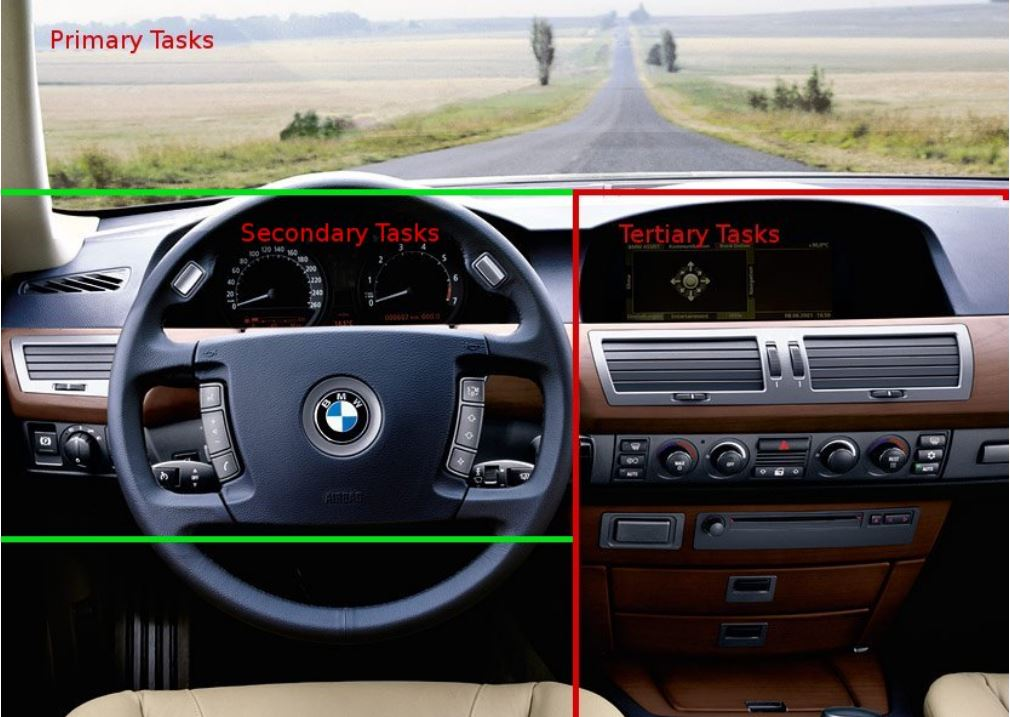
\includegraphics[width=0.5\textwidth]{img/Fahrbereiche_Tonnis.JPG}
	\caption{Aufteilung der Bereiche von primären, sekundären und tertiären Aufgaben. Bild entnommen aus \citet{Tonnis:2006}}
	\label{fig:Fahrbereiche_Tonnis}
\end{figure}
Die wichtigste Aufgabe des Fahrers ist das Fahren an sich, also die sichere Fortbewegung zum Ziel. 
Diese Aufgabe wird als primäre Aufgabe (Primary Task) kategorisiert und beinhaltet das Fahren, Bremsen, Spur halten und Lenken. 
Sekundäre Aufgaben (Secondary Tasks) bilden eine weitere Kategorie.
Sie unterstützen mit Aktionen und Reaktionen die primäre Aufgabe und die Sicherheit des Fahrens.
Hierzu gehören zum Beispiel das Blinken oder das Einschalten des Lichts bei Dunkelheit. 
Die letzte Kategorie sind die tertiären Aufgaben (Tertiary Tasks).
Sie beinhalten alle Aufgaben, die unabhängig vom Fahren gemacht werden können, wie zum Beispiel die Bedienung von Komfortfunktionen, Kommunikationsfunktionen oder Entertainmentfunktionen, aber auch Interaktionen mit dem Beifahrer \citep{geiser1985man}, \citep{Kern:2009}. 
Diese dritte Kategorie ist ein wesentlicher Bestandteil der Ablenkungen des Fahrers und führt oft zu Fahrfehlern oder sogar Unfällen \citep{neale2005overview}, \citep{rumar1988vehicle}. 

\subsection[Design von IVIS]{Design von Informationssystemen im Auto}
Beim Design von Informationssystemen im Auto (IVIS) ist es wichtig im Kopf zu behalten, wer unsere Nutzer sind.
Das Alter von Autofahrern kann sich von 16 bis über 90 Jahren erstreckt. 
In der Gruppe der 21-75 jährigen haben über 80\% einen Füherschein \citep{Green_2002}.
Unsere Nutzergruppe spiegelt also einer sehr große Altersspanne wieder. 
Es ist zu erwarten, dass die verschiedenen Altersklassen mit unterschiedlicher Performanz Aufgaben verrichten \citep{Green_2002}. 
Um Informationssysteme möglichst für jeden leicht verständlich zu gestalten, gibt es bereits viele Richtlinien, Prinzipien und Standards.
Beim Design von Informationssystemen im Auto beachtet sollten diese beachtet werden (siehe unter anderem Alliance of Automobile Manufacturers (AAM) \citep{driver2006statement}, National Highway Traffic Safety Administration (NHTSA) \citep{national2012visual}, European Statement of Principles (ESoP) \citep{national2012recommandationl}, ISO, Society of Automotive Engineers (SAE) oder DIN).
\citet{Green:2012:USI:2390256.2390258} hat dazu auch einige der Standards verglichen und zusammengefasst.

\subsection[Evaluation von IVIS]{Evaluation von Informationssystemen im Auto}
Informationssysteme im Auto können das Fahrverhalten negativ durch Ablenkung beeinflussen. 
Deshalb ist es wichtig solche Systeme zu evaluieren, um den Effekt der Ablenkung, die mentalen Belastung und die Interaktionsdauer zu messen. 
Es gibt verschiedene Methoden um ein neues System oder einen neuen Prototypen zu testen. 
\citet{burnett2008designing} zeigt in seiner Abbildung \ref{fig:Evaluation_of_in_car_computing_devices_Burnett2008} die verschiedenen Evaluationstypen von einer realen Feldstudie auf der Straße bis hin zu Laborstudien. 
\begin{figure}
	\centering
		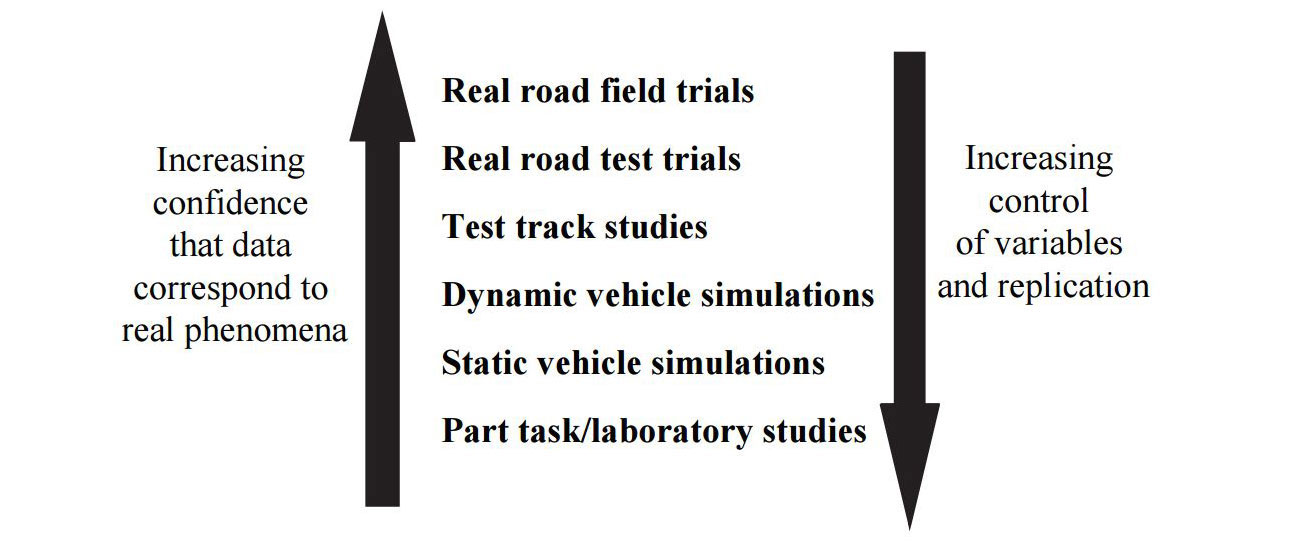
\includegraphics[width=1\textwidth]{img/Evaluation_of_in_car_computing_devices_Burnett2008.jpg}
	\caption[Evaluierungstypen und ihre Abhängigkeit zu Validität und deren Kontrollierbarkeit]{
Evaluierungstypen und ihre Abhängigkeit zur Validität und deren Kontrollierbarkeit. 
Bei realen Feldstudien verhalten sich Fahrer sehr natürlich, jedoch ist es schwer die Beeinflussung von Variablen zu kontrollieren. 
Im Gegensatz dazu können in Laborstudien die Variablen genau kontrolliert werden, jedoch ist das Fahrverhalten konstruiert und entspricht nicht mehr dem natürlichen Verhalten. 
Idee und Bild aus \citet{burnett2008designing}}
	\label{fig:Evaluation_of_in_car_computing_devices_Burnett2008}
\end{figure}

In realen Feldstudien zur Untersuchung des Fahrverhaltens werden die Fahrzeuge zur Erhebung gewünschter Werte instrumentiert und über einen Zeitraum beobachtet. 
Mit dieser Methode können unter realistischen Bedingungen Daten erhoben werden. 
Allerdings können Variablen wie das Wetter oder die Verkehrslage nicht beeinflusst werden. 
In einer High Fidelity Fahrsimulation können äußere Einflüsse wie die Verkehrslage kontrolliert werden, jedoch nimmt hier bereits das natürliche Fahrverhalten ab, da sich der Fahrer offensichtlich in einer Studie befindet und sich möglicherweise anders verhält. 
Außerdem sind die Kosten und der Aufwand einer solchen Studie sehr hoch. 
Eine Low Fidelity Fahrsimulation ist einfacher umzusetzen, jedoch nimmt das realistische Fahrverhalten weiter ab. 
Die Validität der Daten ist bei realen Feldstudien am besten und nimmt bis zu den Laborstudien immer mehr ab. 
Umgekehrt ist die Kontrolle von Variablen und deren Wiederholbarkeit bei Laborstudien am besten und bei realen Feldstudien am unkontrollierbarsten.

Bei der Wahl einer Evaluierungsmethode sollte die Abwägung zwischen Validität der Daten und die Kontrollierbarkeit der Variablen bewusst getroffen werden.

Wir stellen im Folgenden fünf Varianten vor, mit denen IVIS bereits evaluiert wurden. Die 15-Sekunden Regel, der NASA Task Load Index (NASA TLX), der Driving Activity Load Index (DALI), die Okklusions Methode und der Lane-Change Test. 
Diese Varianten können in einem stehenden Fahrzeug getestet werden. 

\subsubsection{15-Sekunden Regel}
Die Länge einer sekundären oder tertiären Aufgabe steht in Korrelation mit dem Unfallrisiko. Da es einfacher ist die Gesamtdauer einer Aufgabe (Total Task Time) zu bestimmen, ist die 15 Sekundenregel eine vereinfachte Annahme, dass eine Aufgabe in einem stehenden Auto nicht länger als 15 Sekunden dauern soll \citep{green199915}. 
Diese Regel ist die Grundlage eines vom Society of Automotive Engineers (SAE) vorgeschlagenen Standards \citep{green1999sae}. 
\citet{green1999sae} definiert die Dauer in einem stehenden Auto oder einer Attrappe gemessen, in dem der Proband nur die gewünschte Aufgabe ausführt. TODO(Satz kapier ich nich)
Das entspricht der Total Task Time, die wir in unserer Studie ebenfalls verwenden werden.

\subsubsection{NASA TLX}
\citet{hart1988development} entwickelte den NASA Task Load Index, dessen Verfahren die mentale Belastung in 6 Dimensionen misst. 
Dafür verwenden wir die deutsche Übersetzung des NASA TLX. 
Die Beanspruchungen werden unterschieden in: 
\begin{enumerate}
	\item \textbf{Geistige Anforderungen:} Wie viel geistige Anstrengung war bei der Informationsaufnahme und -verarbeitung erforderlich (zum Beispiel Denken, Entscheiden, Rechnen, Erinnern, Hinsehen, Suchen)? 
War die Aufgabe leicht oder anspruchsvoll, einfach oder komplex, erforderte sie hohe Genauigkeit oder war sie fehlertolerant?
	\item \textbf{Körperliche Anforderungen:} Wie viel körperliche Aktivität war erforderlich (zum Beispiel Ziehen, Drücken, Drehen, Steuern, Aktivieren)? 
	War die Aufgabe leicht oder schwer, einfach oder anstrengend, erholsam oder mühselig?
	\item \textbf{Zeitliche Anforderungen:} Wie viel Zeitdruck wurde hinsichtlich der Häufigkeit oder dem Takt, mit dem Aufgaben oder Aufgabenelemente auftraten, empfunden? War die Abfolge langsam und geruhsam oder schnell und hektisch?
	\item \textbf{Leistung:} Wie erfolgreich wurde die vom Versuchsleiter (oder dem Probanten selbst) gesetzten Ziele erreicht? Wie zufrieden war der Probant mit seiner Leistung bei der Verfolgung dieser Ziele?
	\item \textbf{Anstrengung:} Wie hart musste Der Probant arbeiten, um den Grad an Aufgabenerfüllung zu erreichen?
	\item \textbf{Frustration:} Wie unsicher, entmutigt, irritiert, gestresst und verärgert (im Gegensatz zu sicher, bestätigt, entspannt und zufrieden mit sich selbst) fühlte sich der Probant während der Aufgabe?
\end{enumerate}
Für jede dieser Beanspruchungen wird ein Wert zwischen 1 (gering) und 20 (hoch) abgefragt. 
Anschließend werden im zweiten Teil noch die 6 Beanspruchungen verglichen. 
Es werden alle Beanspruchungen gegenüber gestellt und der Proband muss sich immer für die Beanspruchung entscheiden, die aus seiner Sicht wichtiger ist. 
Somit wird eine Gewichtung ermittelt, um den Grad der Belastung genauer bestimmen zu können. 
Diese Bestimmung der Beanspruchung mit dem NASA TLX ist weitverbreitet und wird regelmäßig in der Forschung verwendet \citep{hart2006nasa}. 
Teilweise wird die kurzen Version (ohne die Gewichtung durch den zweiten Teil) verwendet. 

\subsubsection{DALI}
Sehr ähnlich zu dem NASA TLX ist der DALI, der sich jedoch auf den automobilen Kontext bezieht und den Beanspruchungswert mit angepasster Gewichtung berechnet. 
Der DALI evaluiert die subjektive mentale Belastung eines Fahrers während der Fahrt \citep{pauzie2008method}, mit oder ohne die Unterstützung eines Informationssystems. 
Eine weitere Technik zur subjektiven Einschätzung der Belastung ist die "`Subjective Workload Assessment Technique"' (SWAT), siehe \citep{reid1982subjective}.

\subsubsection{Okklusions Methode}
Hierbei wird die visuelle Belastung von IVIS für die sekundären Aufgaben gemessen. 
Diese Verschluss Methode soll die Abwendung des Blickes simulieren, die zwischen der Hauptaufgabe dem Fahren und dem Blick zum IVIS passiert. 
Die Hauptidee besteht darin die Sicht, durch Abdeckung, abwechselnd für 1,5 Sekunden zu verhindern und anschließend für 1,5 Sekunden zu ermöglichen. 
Heutzutage gibt es spezielle Brillen mit denen diese Methode durchgeführt werden kann \citep{pettitt2006assessment}.

\subsubsection{Lane Change Test (LCT)}
Dieser Test wurde in Kooperation von DaimlerChrysler und BMW von \citet{mattes2003lane} entwickelt. 
Er misst die Performanz von Doppelaufgaben. 
Der Proband muss eine simulierte Fahraufgabe lösen. 
Diese ist in abstrakter Weise dargestellt und es muss auf einer dreispurigen Autobahn zwischen den Spuren gewechselt werden. 
Wann gewechselt werden muss wird mit Schildern angezeigt und es werden hieraus verschiedenen Zeiten gemessen (wie lange dauert ein Wechsel, wurde jedes mal richtig gewechselt). 
Diese Fahraufgabe löst der Proband zuerst ohne sekundäre Aufgabe.
Dies wird als Referenzwert verwendet. 
Anschließend soll der Proband sowohl die Fahraufgabe bewerkstelligen, als auch das zu Testende IVIS. 
Natürlich hat dabei die Fahraufgabe die höhere Priorität.  
Am Ende können die Zeiten von reiner Fahraufgabe und Fahraufgabe mit IVIS verglichen werden. 
Diese Methode kommt dem natürlichen Fahrverhalten deutlich näher, als der 15- Sekunden Regel und der Okklusion Methode.

\section[Vorhersagemodelle]{Modelle zur Vorhersage von Interaktionszeiten}
Zur Vorhersage von Bedien- oder Interaktionszeiten gibt es verschiedene Ansätze und Modelle. 
In den nächsten Unterkapiteln stellen wir drei Varianten vor. 
Dabei gehen wir vor allem auf das Keystroke-Level Modell und dessen Erweiterungen ein. 

\subsection[Fitts` Law]{Fitts` Law}
Der Psychologe Paul Fitts entwickelte 1954 ein Gesetz, dass die Zeit berechnet, die eine eindimensionale Bewegung einer Strecke zu einem Ziel einer bestimmten Größe benötigt \citep{fitts1954information}. 
\begin{figure}
	\centering
		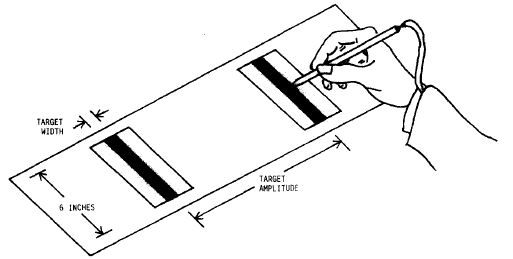
\includegraphics[width=0.7\textwidth]{img/FittsLaw.JPG}
	\caption[Orginaler Aufbau des Versuchs zur Erstellung von Fitts` Law]{Orginaler Aufbau des Versuchs zur Erstellung von Fitts` Law. 
	Die schraffierten Bereiche sollten abwechselnd mit dem Stift getroffen werden, ohne den Bereich zu überschreiten \citep{fitts1954information}. }
	\label{fig:FittsLaw}
\end{figure}

Dieses Gesetz bekam im laufe der Zeit den Namen Fitts` Law und wurde in der Mensch-Maschine Interaktion oft verwendet. 
Die Formel hat ihren Ursprung bei MacKenzie \citep{MacKenzie:1992} und berechnet sich wie folgt:
\[
\text{MT} = a+b * log_2 (\frac{D}{W}+1)
\]
Wobei MT der Bewegungszeit (movement time) entspricht, $a$ und $b$ Konstanten sind, $D$ die Distanz des Startpunkts bis zur Mitte des Zielobjekts ist und $W$ die Breite des Objekts darstellt, die entlang der Bewegungsrichtung gemessen wird. 
Aus Fitts` Law können wir entnehmen, dass Distanz und Bewegungszeit positiv korreliert sind , das heißt mit größer werdender Distanz sich die Zeit verlängert.
Zeit und Größe des Zielobjekt sind dagegen negativ korreliert, das heißt mit größer werdendem Zielobject verkürzt sich die Zeit.
Bei Designentscheidungen kann mit Fitts` Law die schnellere Variante berechnet werden. 
Zum Beispiel bei zwei Konzepten für eine Interface mit unterschiedlich großen Buttons, die unterschiedlich positioniert sind. 

\subsection[GOMS]{GOMS}
Ein weiteres Modell zur Vorhersage von Interaktionszeiten auf einem Bildschirm mit Eingabe durch Tastatur und Maus ist GOMS (Goal, Operator, Method und Selection Rules). 
Bei GOMS wird das Ziel durch ein Set von Methoden und dessen Operatoren erreicht und durch die Selektionsregeln werden die entsprechenden Methoden gewählt \citep{card1983psychology}.
Interaktionsschritte können somit von oben nach unten (top-down) strukturiert und dargestellt werden \citep{butz2014mensch}. 

\subsection{Keystroke-Level Modell (KLM)}
Das Keystroke-Level Modell ist eine vereinfachte Variante von GOMS und baut sich umgekehrt von unten nach oben (bottom-up) auf. 
Das ursprüngliche Keystroke-Level Modell (KLM) wurde von \citet{Card_1980} für Desktopanwendungen mit Tastatur entwickelt. 
Mit dem Keystroke-Level Modell kann die Zeit vorhergesagt werden, die ein Experte benötigt, um eine bestimmte Aufgabe zu lösen. 
Um diese Zeit vorhersagen zu können wird die Aufgabe in ihre Einzelschritte den Operatoren unterteilt und deren Zeiten aufsummiert. 
Diese resultierende Zeit entspricht der "`Total Task Time"', also die Zeit, die benötigt wird bis ein Nutzer die gesamte Aufgabe vollendet hat. 
Das Set von Operatoren besteht aus einen mentalen Operator \textbf{M} und vier physischen Operatoren. 
Der mentale Operator entspricht einer Vorbereitungszeit, die ein Nutzer vor oder zwischen Operatoren benötigt.
\begin{figure}
	\centering
		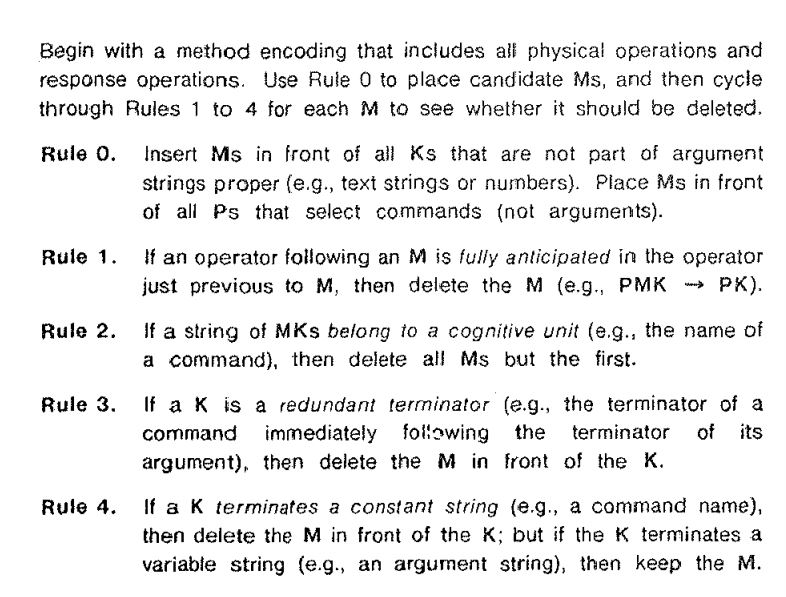
\includegraphics[width=0.7\textwidth]{img/KLM_Mental_Operator_Rules.JPG}
	\caption{Plazierungsregeln des mentalen Operators}
	\label{fig:KLM_OPeratoren}
\end{figure}
Um das Keystroke-Level-Model richtig anzuwenden werden noch Regeln vorgegeben, um den mentalen Operator \textbf{M} richtig zu platzieren. 
Es gibt 5 verschiedene Regeln mit deren Hilfe die Berechnung einer Aufgabe alle benötigten physischen und mentalen Operatoren vorgibt. 
Die 4 physischen Operatoren sind:
\begin{itemize}
	\item \textbf{K (Keystroke)}: Tastenklick
	\item \textbf{P (Pointing)}: Maus zu einem Zielort verschieben
	\item \textbf{D (Drawing)}: ein Set von geraden Linien mit der Maus malen
	\item \textbf{H (Homing)}: der Wechsel zwischen Maus und Tastatur
\end{itemize}
Außerdem gibt es noch den Operator R(t), der die Antwortdauer des Systems darstellt. 

Es wird grundsätzlich bei den Zeiten von Experten ausgegangen, die keine Fehler machen, jedoch werden beim Tippen von Texten (Operator K) 7 Kategorien unterschieden. 
Diese Zeiten haben eine Spanne vom besten Tipper bis zum schlechtesten Tipper, siehe \fref{fig:KLM_OPeratoren}.
\begin{figure}
	\centering
		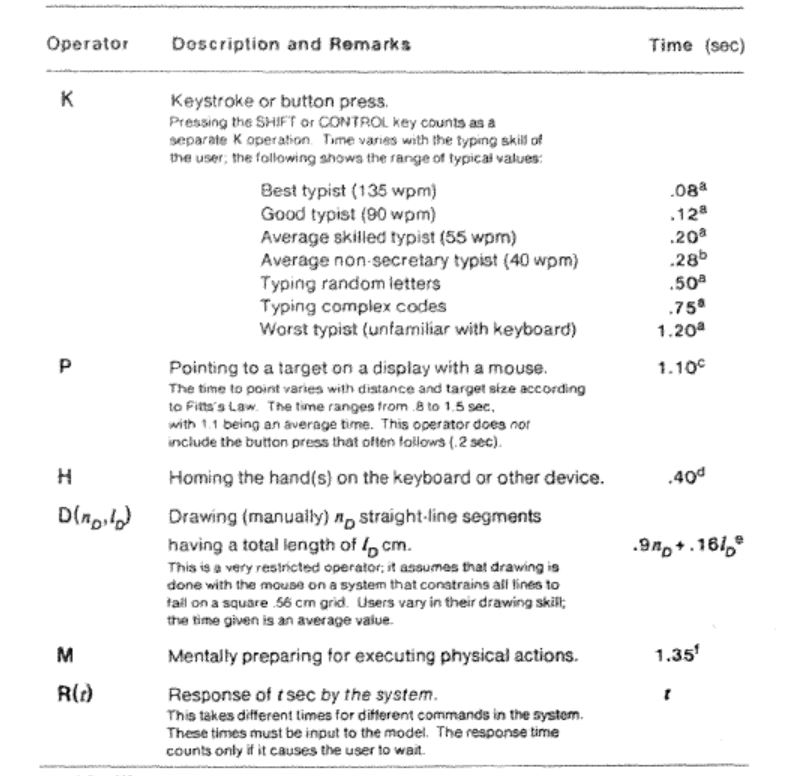
\includegraphics[width=0.7\textwidth]{img/KLM_OPeratoren.JPG}
	\caption{Orginale Tabelle der Operatoren von \citet{Card_1980}}
	\label{fig:KLM_OPeratoren}
\end{figure}

Dieses Modell ermöglicht in einem sehr frühen Stadium der Entwicklungsphase, bereits vor der Implementation, vorherzusagen wie lange Experten für bestimmte Aufgaben benötigen. 
Dieses Modell wurde bereits in vielen Studien angewendet und immer wieder auf Weiterentwicklungen angepasst.
Um bei beliebigen Interfaces schnell und ohne Fehler das KLM zu erzeugen entwickelten \citet{John_2004} ein Tool (später auch CogTool genannt), das von neuen Interfaces das KLM automatisch generiert und somit das Testen von neuen Interfaces noch einfacher macht.

Mit dem Fortschritt der Technik kommen ständig neue Anwendungen mit neuen Modalitäten auf den Markt, die implementiert und getestet werden müssen. 
Deshalb wurde im Laufe der Zeit das KLM immer weiter an aktuelle Geräte und Interfacekonzepte angepasst. 
In den folgenden Abschnitten geben wir eine Zusammenfassung der Erweiterungen des Keystroke-Level Modell.
\subsection[KLM für tragbare Geräte]{Erweiterung des KLM für tragbare Geräte}
\citet{Luo_2005} haben das Modell für tragbare Geräte mit Stiftnutzung statt der Tastatur erweitert beziehungsweise auf diesen Kontext angepasst. 
Die Modelle wurden mit Hilfe der für KLM entwickelten Software CogTool generiert \citep{John_2004}. 
Die vorhergesagten und die gemessenen Zeiten betrugen nur einen Vorhersagefehler von weniger als 8\%.
\citep{Holleis_2007} und \citep{Li_2010} ergänzen das KLM für die Handynutzung. 
\citeauthor{Li_2010} geht dabei mehr auf stiftbasierte Operatoren ein und \citet{Holleis_2007} betrachten mehr die haptischen Tasten auf Handys und führt allgemeinere Operatoren hinzu. 
\citet{Holleis_2007} erweitert das Keystroke-Level Modell unter anderem mit 7 neuen Operatoren, um die Dauer von  fortgeschrittenen Interaktionen auf Handys vorhersagen zu können. 
Diese neuen Operatoren sind:
\begin{itemize}
	\item \textbf{Macro Attencion Shift ($S_\text{Macro}$):} Wechsel zwischen dem Handy und der realen Welt.
	\item \textbf{Micro Attention Shift ($S_\text{Micro}$):} Wechsel zwischen Display, Tastatur und dem Hotkeybereich.
	\item \textbf{Distraction (X):} Ein Ablenkungsfaktor wird mit den Operationen multipliziert.
	\item \textbf{Action (A(t)):} Aktionen, die nicht in Operatoren unterteilt werden können.
	\item \textbf{Gesture (G):} Gestenerkennung wie zum Beispiel das Handy drehen oder Zahlen in die Luft malen.
	\item \textbf{Fingermovement (F):} Fingerbewegung von einer Position zu einer anderen.
	\item \textbf{Initial Act (I):} Zeit um zum Beispiel das Handy aus der Tasche zu holen.
\end{itemize}
Die Operatoren K, P und H des orginalen KLM werden etwas angepasst, M bleibt gleich und D wird nicht benötigt.
 
\citet{Li_2010} kombinieren das KLM mit einem neuen Konzept von Operator Blöcken. 
Ein Operator Block enthält eine Sequenz von Operatoren, die häufig als Einheit in Aktionen vorkommen. 
Dem originalen KLM werden neun physische Operatoren hinzugefügt und fünf mentale Operatoren, wovon vier für die Stiftnutzung angelegt sind. 
Teils entsprechen die physischen Operatoren denen von \citet{Holleis_2007} und teils werden deren Operatoren wieder verworfen. 

\subsection[KLM für Touch]{Erweiterung des KLM für Toucheingaben}
Nachdem bei mobilen Geräten wie Smartphones oder Tablets mehr und mehr die Stiftnutzung verschwindet und eingebaute Touchscreens verwendet werden wurde auch in diesem Bereich das KLM erweitert. 
\citet{Abdulin_2011} untersuchte das KLM für direkten Touch auf 7-17 Zoll großen Tablets. 
Die KLMs von drei verschiedenen Interfaces wurden mit dem CogTool generiert und mit Studienzeiten verglichen. 

Ebenfalls auf Touchscreens fokussieren sich \citet{ElBatran_2014} und \citet{Rice_2014}. \citet{ElBatran_2014} gewinnt in drei Studien Zeiten für drei Touch-Operatoren: Swipe, Zoom und Tap. \citet{Rice_2014} erstellen ein neues Set von Operatoren, dem Touch-Level Modell, zusammen. 
Dafür lassen sie die ursprünglichen Operatoren K, H, M und R(t) unverändert. 
Die Operatoren X und I werden von \citet{Holleis_2007} übernommen und acht weitere Operatoren hinzugefügt: 
\begin{itemize}
	\item \textbf{Gesture (G)}: Geste mit 1, 2 oder mehreren Fingern
	\item \textbf{Pinch (P)}: 2-Fingergeste, wobei die Finger am Ende geschlossen sind
	\item \textbf{Zoom (Z)}: 2-Fingergeste, wobei die Finger am Anfang geschlossen sind
	\item \textbf{Tap (T)}: Finger-Tap
	\item \textbf{Swipe (S)}: Finger auf dem Touchscreen bewegt sich in horizontaler oder vertikaler Richtung
	\item \textbf{Tilt (L(d))}: Neigung oder Rotation des ganzen Geräts um d Grad
	\item \textbf{Rotate (O(d))}: 2-Fingergeste mit der auf dem Screen etwas um d Grad rotiert wird
	\item \textbf{Drag (D))}: 1-Fingergeste mit der meist ein Objekt von einer Position zu einer anderen gebracht wird
\end{itemize}
Das Touch-Level Modell soll in zukünftigen Studien noch verifiziert und evaluiert werden.
\subsection[KLM im automobilen Kontext]{Erweiterung des KLM im automobilen Kontext}
Die Infotainmentsysteme in Autos werden immer komplexer und auch hier ist es wichtig für Designer in einem frühen Stadium Interfaces testen zu können. 
Es gibt im Auto nicht nur ein Gerät das betrachtet werden kann, sondern mehrere Bereiche mit verschiedensten Bedienelementen. 
Diese Bedienelemente können ursprüngliche haptische Knöpfe und Schalter sein, aber auch Touchdisplays und mögliche Einrichtungen für Sprach- oder Gestensteuerungen. 

\citet{Pettitt_2007} befassen sich 2007 mit diesem Thema und erweitern das KLM für Informationssysteme im Auto, mit Hinzunahme der Occlusion Technik. 
Die Zeiten dieses KLM werden dann mit den Zeiten von einer Occlusion Studie verglichen. 
Sie verwenden die Operatoren von \citet{Card_1980} und der Operator $R_f$ (Reach far) wurde von \citet{Green_2002} adaptiert, genau wie der Operator (Reach near), dessen Zeit für die Bewegung innerhalb eines Systems mit Fitt's Law berechnet wird.

Ebenfalls im automobilen Kontext erweitert \citet{schneegass_2009} (siehe auch \citep{SchneegaB_2011}) das KLM und bezieht sich dabei im speziellen auf die Interaktionen von Autoradios. 
In dieser Studie werden vier Aufgaben in diesem Kontext mit insgesamt 78 Operatoren aufgezeichnet und deren Zeiten berechnet. 
Der interessanteste und für den automobilen Kontext neu hinzugefügte Operator ist der Turn (T) Operator. 
Dieser Operator wird für alle haptisch drehbaren Knöpfe verwendet und es wurden jeweils drei verschiedene Drehwinkel für Linksdrehungen (negativ) und Rechtsdrehungen (positiv) untersucht ($-180^\circ$, $-90^\circ$, $-45^\circ$, $45^\circ$, $90^\circ$, $180^\circ$). 
\begin{figure}[ht]
  \centering
  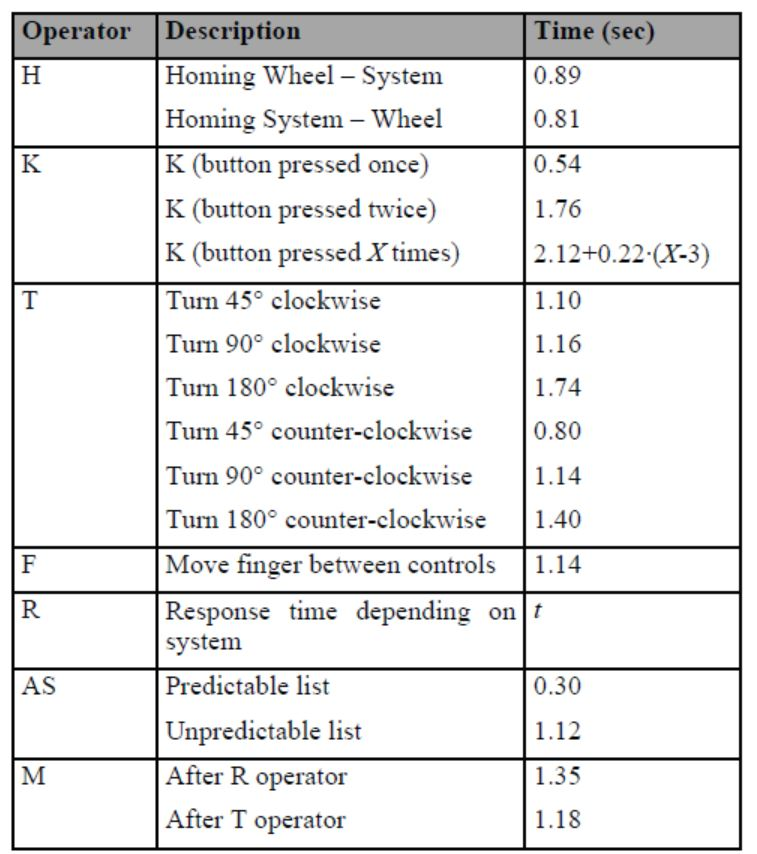
\includegraphics[width=0.7\textwidth]{img/Schneegass_KLM_Operator_Table.jpg}
  \caption[Tabelle der Operatorzeiten von Schneegaß]{Tabelle der Operatoren, deren Beschreibung und den dazugehörigen Zeiten.}
  \label{fig:Bild1}
\end{figure}

Schneegaß verweist darauf, dass die Berechnung der Zeiten für den Turn(T) Operator in Zukunft noch genauer untersucht werden sollte, indem zusätzlich unterschieden wird, ob in einen bestimmten Bereich gedreht oder ein bestimmter Winkel der Drehung verlangt wird. 
Die genauen Zeiten der einzelnen Operatoren können aus \fref{fig:Bild1} von \citet[Seite 75]{SchneegaB_2011} entnommen werden. 
Ein weiterer wichtiger Aspekt aus seinen Ergebnissen ist das Feedback der Teilnehmer dieser Studie. Es wurde angemerkt, dass die Aufgaben, mit bis zu sechs Unteraufgaben, zu lang waren. 
Somit war die kognitive Auslastung, sich diese Aufgaben zu merken, zu hoch. 
Außerdem reagierte das verwendetet System langsamer, als die Teilnehmer es von eigenen Autos gewohnt waren. 
Dieses Feedback versuchen wir in unserer Studie aufzugreifen, indem wir die Aufgaben möglichst kurz halten. 

\section[Multimodale Interaktion]{Multimodale Interaktion}
Multimodale Interaktion ist für Menschen etwas ganz natürliches, das unbewusst bei den meisten Kommunikationen zwischen Menschen gemacht wird. 
Zwei Leute unterhalten sich zum Beispiel und nebenbei zeigt einer zusätzlich auf einen Gegenstand, schauen in eine Richtung und kombinieren all diese zusätzlichen Informationen, die das gesamte Gespräch bereichern und erleichtern. 
Um unsere Außenwelt besser verstehen zu können schauen, hören, tasten und riechen wir zugleich \citep{sharma1998toward}. 
Um auch Interaktionen zwischen Mensch und Maschine intuitiver und natürlicher für zu gestalten könnte das Hinzufügen zusätzlicher Modalitäten eine große Bereicherung sein.

Multimodale Systeme können durch mehrere Kommunikationskanäle bedient werden. 
Die Mensch Maschine Interaktion geschieht zwischen den Aktoren und Sensoren des Menschen, siehe Grafik \ref{fig:Multimodalitaet}von \citep{neuss_2001}.
\begin{figure}
	\centering
		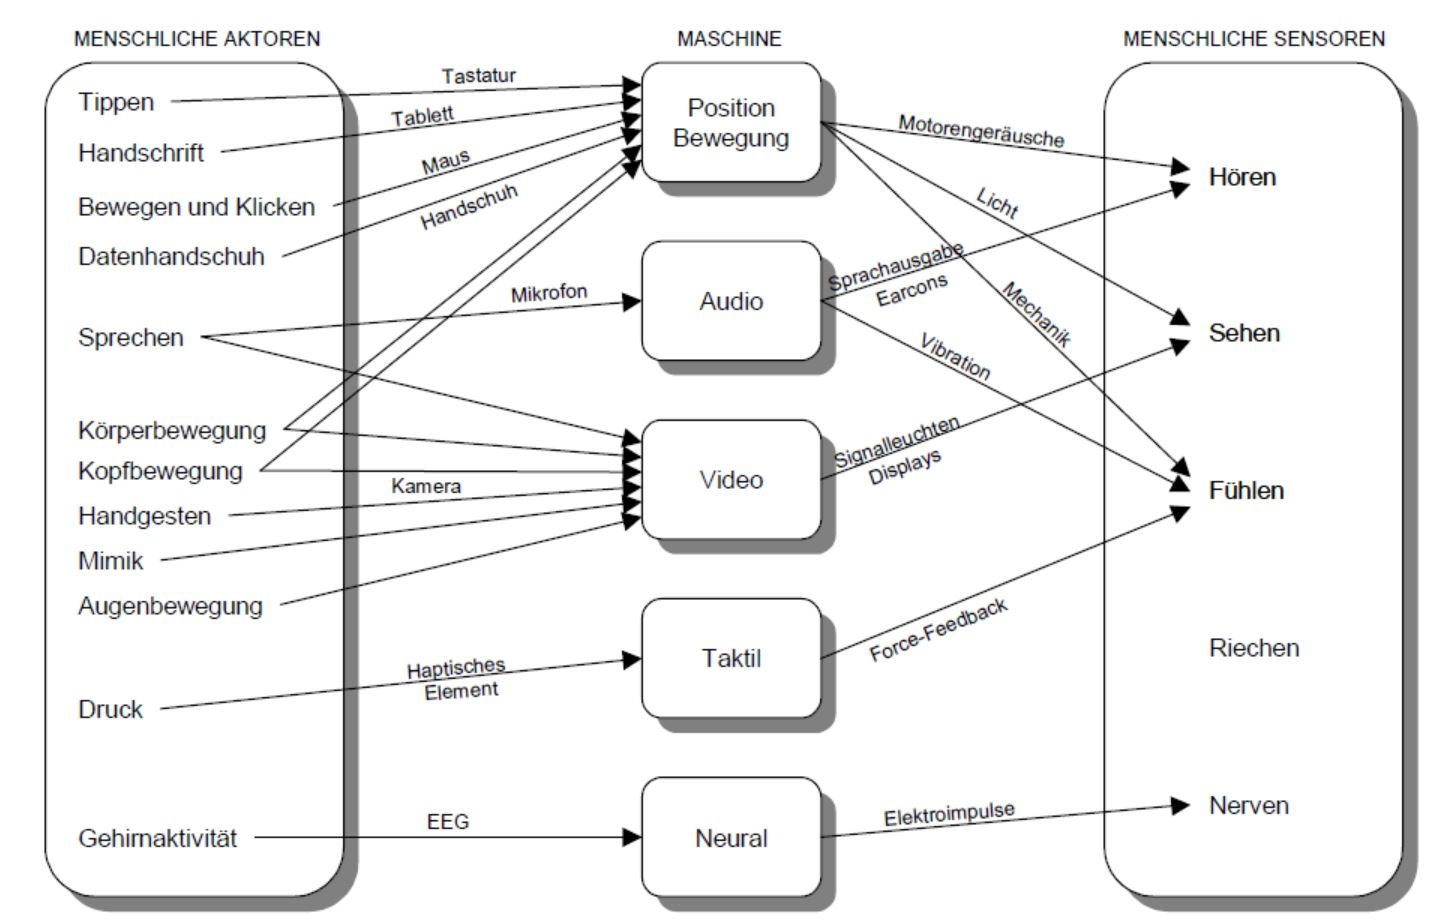
\includegraphics[width=1\textwidth]{img/Multimodalitaet.JPG}
	\caption[multimodale Kommunikationskanäle]{Die Abbildung von \citep{neuss_2001} beschreibt das Zusammenspiel von menschlichen Aktoren und Sensoren in Interaktion mit der Maschine. Das Modell ist abgeleitet von \citep{sharma1998toward}}
	\label{fig:Multimodalitaet}
\end{figure}
Doch wann kann ein Nutzer eine bestimmte Modalität verwenden oder zu einer anderen wechseln?
\citet{neuss_2001} differenziert in seiner Dissertation vier verschiedenen Ausprägungen der Multimodalität hinsichtlich der Eingabe.
\begin{itemize}
	\item \textbf{seriell-redundant:} Modalität kann beliebig gewechselt werden
	\item \textbf{seriell-exklusiv:} Modalität kann nur nach bestimmten Schritten gewechselt werden
	\item \textbf{parallel-ergänzend:} "`Simultan getätigte Eingaben mit verschiedenen Modalitäten ergänzen sich."'\citep{neuss_2001}
	\item \textbf{parallel-verifizierend:} "`Simultan getätigte Eingaben mit verschiedenen Modalitäten bestätigen sich gegenseitig"' \citep{neuss_2001}. Ein Beispiel wäre die Kombination aus Sprache und Lippenlesen.
\end{itemize}
Je nach Kontext wird die beste Variante gewählt. 
Alle Varianten, ob alleine oder in Kombination geben dem Nutzer mehr Freiheit das Ziel zu erreichen und erhöhen zudem die Effizienz \citep{neuss_2001}. 

Eine Herausforderung ist ein gutes Design von multimodalen Interfaces, sodass die Vorteile der Modalitäten genutzt werden können, aber auch die Bedienung den Nutzer unterstützt und nicht verwirrt. 
Dazu haben \citet{Reeves_2004} ein Regelwerk für das Design von multimodalen Interfaces erstellt. 
Deren Ziel ist es, dass in Zukunft Interaktionen natürlicher und intuitiver werden und die Robustheit durch redundante Informationen und Interaktionsmodalitäten gesteigert wird. 
Einige wichtige Aspekte sind hierbei das konsistente Design von Input und Output. 
Es soll zum Beispiel vermieden werden, dass redundante Informationen in verschiedenen Modalitäten präsentiert werden, wenn der Nutzer sich dabei auf zwei verschiedene Quellen konzentrieren muss. 
Der Output soll im gleichen Stil des Inputs gestalten werden. 
Außerdem ist es wichtig, dass ein multimodales Interface Design adaptiv und konsistent ist. 
Es soll ausreichend Feedback geben und eine gute Fehlerbehandlung lässt den Nutzer immer wissen, welche Fehler ihn zu einem Status gebracht haben. 

\section[Multimodale Interaktion im Auto]{Multimodale Interaktion im automobilen Kontext}
Multimodale Interaktion gibt es bereits in aktuellen Autos und dieser Bereich umfasst ein großes Feld an Möglichkeiten. 
Eine der bekanntesten Varianten multimodaler Interaktion im Auto, ist die Sprachbedienung mit der zum Beispiel Anrufe getätigt werden. 
Auch Touchdisplays von externen Navigationssystemen oder Informationssystemen werden immer häufiger verwendet. 
Einige interessante Forschungsansätze von multimodaler Interaktion im Auto stellen wir Ihnen vor.

\citet{Pieraccini_2004} entwickelte einen multimodalen Prototypen in einen Ford Model U. Dieser basiert auf ein sprach basiertes System, dass durch einen visuellen und haptischen Touch-Screen unterstützt wird. 
Diese Kombination soll Anfängern das Erlernen von Sprachbefehlen erleichtern, indem visuell Hilfen der Sprachbefehle auf dem Touch-Screen in jeder Ebene des Interfaces zu sehen sind. 
Für Experten ist die Nutzung von ganzen Sätzen möglich, ohne für jede Ebene ein eigenes Kommando verwenden zu müssen.
Nach jedem Sprachbefehl ist es möglich durch eine Touch-Geste den Modus zu Wechseln. 

Redundante Modalitäten haben viel Potenzial für das Design von modernen Interfaces, wie auch \citet{Muller_2011} in ihrem Artikel feststellten haben sie zwei signifikante Vorteile im Gebrauch von Autos: Es ist zu einem dem Fahrer möglich, die für ihn passenste Modalität je nach Situation zu wählen. 
Zum anderen können lange Interaktionen, von einer Modalität zur anderen, ohne Probleme gewechselt werden.

\citet{Bertoldi:2010} haben die Multimodalität in Fahrer Assistenz Systemen untersucht, mit dem Ergebnis, dass es in diesem Feld noch viel zu Forschen und zu verbessern gibt. 
Aber es hat das Potenzial die Sicherheit zu erhöhen, die Reaktionszeiten und die Eyes-off-the-road Zeit zu verkürzen und das Bewusstsein der Fahrersituation zu erhöhen. 

\citet{Doring:2011} erweiterten ein Lenkrad in der Mitte mit einer Multi-Touch Oberfläche und untersuchten deren Möglichkeiten für Touch-Gestensets. 
Die visuelle Ablenkung konnte durch Touchgesten reduziert werden. 

Eine ähnliche Idee hatten \citet{Pfleging_2012}. 
Sie entwickelten, unter Rücksichtnahme von guter Lernbarkeit, Sichtbarkeit, Granularität und der Möglichkeit Aktionen rückgängig zu machen, ein im Lenkrad integriertes multimodales System, das Sprache und Touchgesten kombiniert. 
Es stellte sich heraus, dass Sprache und Gesten langsamer sind als der Gebrauch von haptischen Buttons, jedoch bei ähnlicher Fahrperformanz die visuelle Anstrengung geringer ist. 
Ein Nachteil ist das nötige Erlernen und Erinnern von Sprachbefehlen und Gesten. 
In deren System wurde zuerst die Sprache verwendet um Objekte oder Funktionen direkt ohne hierarchische Struktur zu benennen und anschließend konnte mit einer Touchgeste deren Parameter justiert werden, siehe auch \citep{Pfleging_t_2011}. 
Bei den Sprachbefehlen wurden von 82,1\% die Benennung von Objekten bevorzugt. 
Bei den Touchgesten benutzten 78,1\% der Teilnehmer 1-Finger Touchgesten. 

\citet{stracke2014touch} untersuchte in seiner Bachelorarbeit Touch Interactionen auf der Mittelkonsole. 
In dieser Arbeit wurde Direct-Touch-Steuerung mit "`drei Formen positionsunabhängigen Wischgesten"' \cite[Seite 57]{stracke2014touch} dem Serial Swipe, dem Relative Swipe und einem Relative Swipe mit Multi-Touch verglichen. 
Mit der Direct-Touch-Variante konnte eine Verkürzung der Interaktionszeit festgestellt werden. 
Jedoch schnitt diese Variante bei der Fehlerrate schlechter als die anderen Varianten ab, allerdings konnte keine Signifikanz bewiesen werden. 
Sehr beliebt war die Direct-Touch-Steuerung zur Einstellung der Luftverteilung und für Ein-/Ausschaltoptionen. 

Im nächsten Schritt verschaffen wir uns in einem Workshop einen Überblick über multimodale Interaktionen im Auto.

\chapter[Workshop Connected Minds]{Workshop zur Bestimmung eines Aktionssets}\label{cha:Workshop}
Um ein Konzept für unser Modell abzuleiten, interessiert uns welche Arten von Interaktionen, in einem Auto stattfinden und aus welchen Einzelschritten diese bestehen. Darüber hinaus wollen wir aktuelle und mögliche Umsetzungen der Modalitäten Haptik, Touch, Sprache und Gestik zu den Einzelschritten sammeln. Die Interaktionen sollen in die Kategorien Kommunikation, Navigation, Medien, Komfortfunktionen und Einstellungen unterteilt werden.

Zu diesem Zweck wollen wir im Rahmen eines Workshops unsere Ziele erarbeiten. Dafür ist eine Fokusgruppe geeignet, die sich im automobilen Bereich befindet.   
Bei BMW gibt es jeden Mittwoch die Möglichkeit eine Brainstorming Runde (Connected Minds) mit freiwilligen internen Mitarbeitern anzumelden. Diese Möglichkeit nutzen wir, um unseren Workshop durchzuführen.
Am 24.08.2016 führten wir mit insgesamt neun Teilnehmern unseren Workshop durch. 
Wir bereiteten unsere Ziele vor, die es zu erreichen galt. Die Ziele lauten wie folgt:  
\begin{enumerate}
	\item \textbf{Ziel:} Anwendungsbeispiele von Interaktionen im Auto sammeln und diese einer der Kategorien zuordnen (Kommunikation, Navigation, Medien, Komfortfunktionen und Einstellungen). Anschließend diese in ihre einzelnen Aktionen zerlegen. 
	\item \textbf{Ziel:} Aus den Anwendungsbeispielen die Aktionen gruppieren und Umsetzungen für die verschiedenen Modalitäten (Haptik, Sprache, Touch und Geste) finden beziehungsweise sammeln.
\end{enumerate}
\section[Ablauf]{Organisation und Ablauf des Workshops}
\begin{figure}[ht]
  \centering
  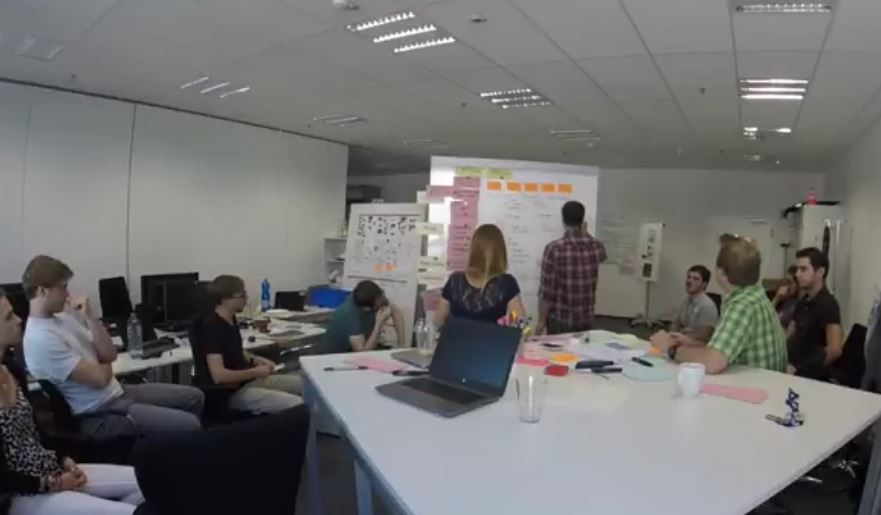
\includegraphics[width=1\textwidth]{img/ConnectedMind.jpg}
  \caption{Connected Minds bei BMW}
  \label{fig:ConnectedMind}
\end{figure} 
Nach einer kurzen Vorstellrunde wurden die Teilnehmer in das Thema eingewiesen und die zwei zu erreichenden Ziele vorgestellt. 
Für das erste Ziel sammelten wir im ersten Schritt Anwendungsbeispiele und ordneten sie den Themengebieten Kommunikation, Navigation, Medien, Komfortfunktionen oder Einstellungen zu (siehe \fref{fig:ConnectedMindErgebnisse} linkes Bild).
\begin{figure}[ht]
  \centering
  \includegraphics[width=1\textwidth]{img/ConnectedMindsErgebnis.jpg}
  \caption[Connected Minds Ergebnisse]{Connected Minds Ergebnisse - Ziel 1 (links), Ziel 2 (rechts)}
  \label{fig:ConnectedMindErgebnisse}
\end{figure}  

Als nächsten Schritt gliederten wir jedes Anwendungsbeispiel in die jeweiligen Aktionen, wobei wir darauf achteten, dass sie möglichst abstrakt und vom Interface unabhängig formuliert wurden. 
Ein Beispiel hierfür ist Abfolge von etwas Auswählen, Inkrementieren und Bestätigen. 
Die gesammelten Aktionen wurden für das zweite Ziel gruppiert und anschließend auf einer neuen Tafel untereinander gepinnt. 
Für jede Aktion wurden sowohl aktuell bestehende als auch potentiel mögliche Umsetzungen für die Modalitäten Haptik, Touch, Geste und Sprache gesammelt (siehe \fref{fig:ConnectedMindErgebnisse} rechtes Bild und \fref{tab:table1}). 

Um die Ziele zu erreichen benötigten wir insgesamt 1,5 Stunden, wobei das erste Ziel nach 30 Minuten erfüllt wurde und das zweite Ziel eine Stunde benötigte. 
Der Workshop wurde auf Video aufgezeichnet.
\section[Ergebnisse des Workshops]{Ergebnisse des Workshops Connected Minds}
Es haben sich sechs verschiedene Aktionen herauskristallisiert, aus denen alle Bedienbeispiele zusammengesetzt werden können.
\begin{itemize}
	\item \textbf{Bestätigung (B):} Eingabe oder Auswahl bestätigen.
	\item \textbf{Direktauswahl (DA):} Auswahl aus sichtbaren Elementen.
	\item \textbf{Ein-/Ausschalten (E/A):} Ein- und Ausschalten oder Aktivieren und Deaktivieren von Funktionen.
	\item \textbf{Listennavigation (L):} Seitenweise inkrementieren und anschließende Direktauswahl (DA).
	\item \textbf{De-/Inkrementieren (Inkr):}  Scrollen, Erhöhen/Verringern von Werten.
	\item \textbf{Texteingabe (T):}  Wiederholte Eingabe eines Buchstabens und anschließende Bestätigung (B).
\end{itemize}

\begin{table}[ht]
	\centering
	\begin{tabular}{|l|l|l|l|l|}
		\hline
		Aktion & Haptik & Touch & Gesten 			& Sprache\\
		\hline
				\multirow {3}{*}{B}
					& Button drücken		& Tap 				& Daumen hoch, 									& Ja,\\
					& Dreh-Drücker			& 						& Tauch OK, 										& OK,\\
					& 									& 						& bestimmte Geste halten 				& passt\\
		\hline
				\multirow{2}{*}{DA}
					& Button drücken		& Swipe  			& 3D-Pointing 								& Objekt/Funktion \\
					& Dreh-Drücker			& Tap					& 														& benennen \\		
		\hline
				\multirow{2}{*}{E/A}
					& Button (on/off)		& Tap,  			& von offener zu 								& Funktionsname\\
					& Kippschalter			& Swipe				& geschlossener Hand						& "`ein"'/"`aus"'\\
		\hline
				\multirow{3}{*}{L}
					& Button drücken		& Swipe				& relative  										& hoch/runter mit\\
					& 									& 						& Handbewegung									& Start/Stop,\\
					& Dreh-Drücker			& Tap 				& (Wischgeste, Swipe), 					& weiter/zurück,\\
					& 									& Scroll			& Drehbewegung des Fingers 			& Tonhöhe variieren\\		
		\hline
				\multirow{3}{*}{Inkr.}		
					& Button drücken		& Swipe				& relative Handbewegung 				& hoch/runter mit\\
					& 									& 						& 															& Start/Stop,\\
					& Dreh-Drücker			& Tap 				& (Wischgeste, Swipe), 					& weiter/zurück,\\
					& Hebel drücken			& Scroll			& Drehbewegung des Fingers			& Tonhöhe variieren\\					
		\hline
				\multirow{3}{*}{T}
					& Tastatur					& X mal Tap 	& In der Luft schreiben, 				& diktieren,\\
					& Dreh-Drücker			& Schreiben		& 3D-Pointing auf Tastatur,			& sprechen\\		
					& Morsecode					& 						& L auf Tastatur								&  \\	
		\hline			
  \end{tabular}
	\caption{Ergebnisse der Umsetzungsmöglichkeiten der Modalitäten für die verschiedenen Aktionen}
	\label{tab:table1}
\end{table}
Für die sechs Aktionen wurden für die Modalitäten Haptik, Touch, Geste und Sprache vorhandene oder mögliche Umsetzungen gesammelt. 
\fref{tab:table1} listet alle Vorschläge der verschiedenen Modalitäten auf.
Wir entschieden uns bei dem Touchmodus immer für den direkten Touch auf einem Display. TODO(den satz laenger und umformulieren) 
In der schon erwähnten Bachelorarbeit von \citet{stracke2014touch} erwiesen sich diese Varianten bei Touch für eine gute Umsetzung mit schnellen Interaktionszeiten. 
Auch \citet{Rumelin:2013} bekamen beim direkten Touch die besten Zeiten für das vollenden einer Aufgabe.

Um den Umfang der geplanten Studie im realistischen Bereich zu lassen, haben wir uns entschieden die Haptik als Modalität nicht miteinzubeziehen. 
Unser Fokus soll bei den Modalitäten Touch, Geste und Sprache liegen, auch weil die Haptik im automobilen Kontext bereits in Studien untersucht wurde, siehe \citep{Pettitt_2007}, \citep{schneegass_2009} und \citep{SchneegaB_2011}. 
Die haptische Bedienung stellt natürlich weiterhin einen wichtigen Bestandteil der Interaktion im Auto dar. Da dieser Bereich für uns wegfällt benötigen wir somit die Aktion Ein- und Ausschalten nicht. 
Im nicht haptischen Kontext unterscheidet sich diese Aktion nicht von einer gewöhnlichen Aktivierung eines Buttons.
\paragraph{Geeignete Anwendungsbeispiele:}
Aus den im Workshop genannten Beispielen suchten wir fünf stellvertretende Beispiele heraus, die sowohl alle Aktionen abdecken, als auch zu einem der fünf Themengebiete Navigation, Medien, Komfortfunktionen, Einstellungen und Kommunikation zuzuordnen sind. 
\begin{itemize}
\item navigieren zu Rom, Dorfweg und Kirchengasse (Navigation): DA (Navigation) + DA (Zieleingabe) + T (Ziel) + B (bestätigen)
\item Song "`Happy"' aus beliebten Songs wählen (Medien): DA (Medien) + DA (beliebte Songs) + L ("`Happy"' suchen) + DA ("`Happy"' auswählen)
\item Temperatur um $3^\circ$ erhöhen (Komfortfunktionen): DA (Temperatur) + Inkr. (+ $3^\circ$)
\item Lautstärke erhöhen (Einstellungen): DA (Einstellungen) + Inkr. (von 50\% auf ca. 80\%)
\item Maria Müller aus Kontakten anrufen (Kommunikation): DA (Telefon) + DA (Kontakte) + L ("`Maria Müller"' suchen) + DA ("`Maria Müller"' auswählen)
\end{itemize}
Bei der Einstellung der Lautstärke haben wir uns bewusst für eine grobe Angabe geeinigt (Lautstärke in einem Intervall zwischen 75\% und 85\% erhöhen), da eine genaue Angabe (zum Beispiel um 3 Einheiten verringern) eine unnatürliche Veränderung wäre \citep{stracke2014touch}. 
Unsere Anwendungsbeispiele stellen übliche Anwendungen dar und sind teils in vereinfachter Weise dargestellt, um eine zu hohe kognitive Belastung zu vermeiden. 
Da die Zeiten von Experten gemessen werden sollen, ist es wichtig Fehler und zu lange Bedenkzeiten zu eliminieren und zu minimieren.

Die Inkrementation eines Wertes stellen wir in unseren Beispielen in zwei verschiedenen Varianten dar. 
Einmal soll die Temperatur um 3 Grad erhöht werden, indem durch dreimaliges inkrementieren schrittweise der Wert verändert wird. 
Im Beispiel die Lautstärke von 50\% auf ca. 80\% zu inkrementieren wählen wir einen Slider als Darstellung. 
Hier muss nicht eine Aktion 30 mal angewendet werden, um von 50 auf 80 zu inkrementieren, sondern eine direkte Inkrementation (für die Modalitäten Touch und Geste) soll den Wert verändern. 
Wir unterscheiden also die schrittweise Inkrementation (Inkr. (s)), die für kleine Wertunterschiede Sinn macht und eine direkte Inkrementation (Inkr. (d)), die bei größeren und gröberen Wertunterschieden sinnvoll ist.

Bei der Texteingabe eines Ziels haben wir zur Unterscheidung von kurzen und langen Wörtern 3 verschiedene Ziele mit unterschiedlicher Länge gewählt (Rom, Dorfweg und Kirchengasse). 
Außerdem wurde darauf geachtet möglichst einfach zu schreibende Wörter zu verwenden, um negative Einflüsse in Bezug zu Rechtschreibkenntnissen zu vermeiden. 
Es soll in erster Linie die Zeit gemessen werden, die es benötigt einen Button in bestimmter Größe zu treffen. 
Die mentale Zeit sollte sich auf die Interaktion und das Interface beziehen und nicht auf die Rechtschreibung. 
\section[Idee des Modells]{Abgeleitete Idee für ein multimodales Modell}
Mit unserem Modell sollen sich multimodale Interaktionszeiten vorhersagen lassen, indem sie sich aus den Aktionen Direktauswahl aus sichtbaren Elementen (DA), Bestätigung (B), Listennavigation (L), schrittweiser Inkrementation (Inkr.(s)), direkter Inkrementation (Inkr.(d)), und der Texteingabe (T) zusammensetzen. 
Je nach Modalität unterscheiden sich die Zeiten einer Aktion. 
Außerdem wollen wir herausfinden, welche Kosten bei einem Wechsel von einer Modalität zu einer anderen entstehen. 
Eine Aktion soll in unserem Fall eine durchschnittliche Dauer darstellen, die ein geübter Nutzer benötigt in einem bestimmten Modus die Aktion fehlerfrei auszuführen. 
Ob ein Nutzer sich dabei Zeit lässt oder einmal mehr oder weniger die Hand vom Interaktionsbereich zurück zum Lenkrad nimmt stellt dabei keinen Fehler dar, sondern soll mit in den durchschnittlichen Zeiten berücksichtigt werden. 

Bei den Keystroke-Level Modellen auf Operatorebene gibt es eine "`richtige"' Lösung mit einer bestimmten Anzahl an Operatoren. 
Das ist der schnellste Weg, den Experten verwenden, um eine bestimmte Aufgabe zu lösen. 
Doch bei Interaktionen im Auto lässt sich viel schwieriger eine Abfolge von Operatoren bilden. 
Je nach Nutzer und Situation im Auto werden zum Beispiel mehrere Bewegungen vom Lenkrad hin zum Interaktionsbereich gemacht als nötig. 
Deshalb erscheint es uns eine gute Annäherung die Gesamtdauer in unserem Modell nicht durch Operatoren, sondern durch Aktionen zusammenzusetzen. 
Die Wechselkosten, die wir ebenfalls in unserem Modell berechnen und berücksichtigen wollen enthalten unter anderem einen mentalen Operator und einen Homing Operator \citep{Card_1980} bzw. einen Reach Far Operator \citep{Green_2002}. 
Wie bei dem KLM soll auch bei unserem Modell von Experten ausgegangen werden. 
Es sollen nur Durchgänge gewertet werden, die keine Fehler vom System oder dem Nutzer mit dem System aufweisen.

\chapter[Multimodaler Prototyp]{Umsetzung des multimodalen Prototyps}\label{cha:Prototyp}
Im nächsten Schritt sollen die Anwendungsbeispiele in geeigneter Weise umgesetzt werden, um in einer Studie Interaktionszeiten erheben zu können. 

Unser erster Ansatz war das Interface als Klickdummy zu erstellen und mit der "`Wizard of Oz"' Methode umzusetzen \citep{salber1993applying}. 
In der "`Wizard of Oz"' Methode simuliert der sogenannte "`Wizard"' die Funktionalität eines Systems, indem er Events durch seine Beobachtungen manuell auslöst. 
Das heißt die Funktionalität, bestimmte Gesten oder Sprachbefehle zu erkennen, muss in diesem Fall nicht implementiert werden und ist somit auch nicht anfällig für Fehler. 
Dies ist ein großer Vorteil für ein Modell, dass von Experten ausgeht, die mit dem System vertraut sind und keine Fehler machen. 
Auch Fehler des Systems können mit dieser Methode ausgeschlossen werden. 

Da in der "`Wizard of Oz"' Methode, Events nur durch den "`Wizard"' ausgelöst werden können, ist es schwieriger diese Events zu protokollieren. 
Studien dieser Art werden meist per Video aufgezeichnet und anschließend mit einer Videoanalyse ausgewertet. 
Natürlich gibt es einige Hilfen, um eine Videoanalysen zu optimieren, allerdings bleibt der Zeitaufwand hoch, weshalb wir uns dafür entschieden haben diese Methode nicht zu verwenden. 
Mit einem vollständig funktionsfähigem Prototypen können Events mit Zeitstempeln protokolliert werden, um später die Zeiten für unsere Aktionen und deren Wechselkosten berechnen zu können. 

Im folgenden werden die Anwendungsbeispiele und deren Implementation erläutert.

\section[Anwendungsbeispiele]{Beschreibung und Umsetzung der Anwendungsbeispiele}
Die im Workshop erarbeiteten Anwendungsbeispiele werden in vereinfachter und abstrakter Darstellung im Prototypen umgesetzt. 
Damit wollen wir vermeiden, dass ein auffälliges Design den Nutzer ablenkt. 
Es sollen lediglich die Interaktionszeiten untersucht werden und nicht eine bestimmte Umsetzung eines Interfacedesigns. 
In \fref{fig:UseCases} werden die Anwendungsbeispiele gezeigt welche im Folgenden beschrieben werden, ohne auf die Verwendung der Modalitäten einzugehen. 
Auf die Modalitäten gehen wir im Abschnitt Implementation unter der jeweiligen Modalität ein. 

Diese vier Anwendungsbeispiele sollen in der Studie sowohl unimodal, als auch mit allen multimodalen Kombinationen getestet werden. 
Jeder Proband kann sich in einem Probedurchgang mit der Aufgabe vertraut machen.
Anschließend folgen zwei Messdurchgänge, in denen die Interaktionszeiten erhoben werden. 

In \fref{fig:UseCases} werden die vier umgesetzten Anwendungsbeispiele in einer Übersicht horizontal dargestellt. 
Hier wird auch deutlich, ab welchen Screens ein Modalitätswechsel stattfinden soll. 
Der Modalitätswechsel wurde festgelegt und ist immer mit einem Screenwechsel verbunden. 
Durch diese Vorgabe ist unser Prototyp exklusiv redundant, da nur innerhalb eines Screens die Modalität gewechselt werden soll. 
\begin{figure}[ht]
  \centering
  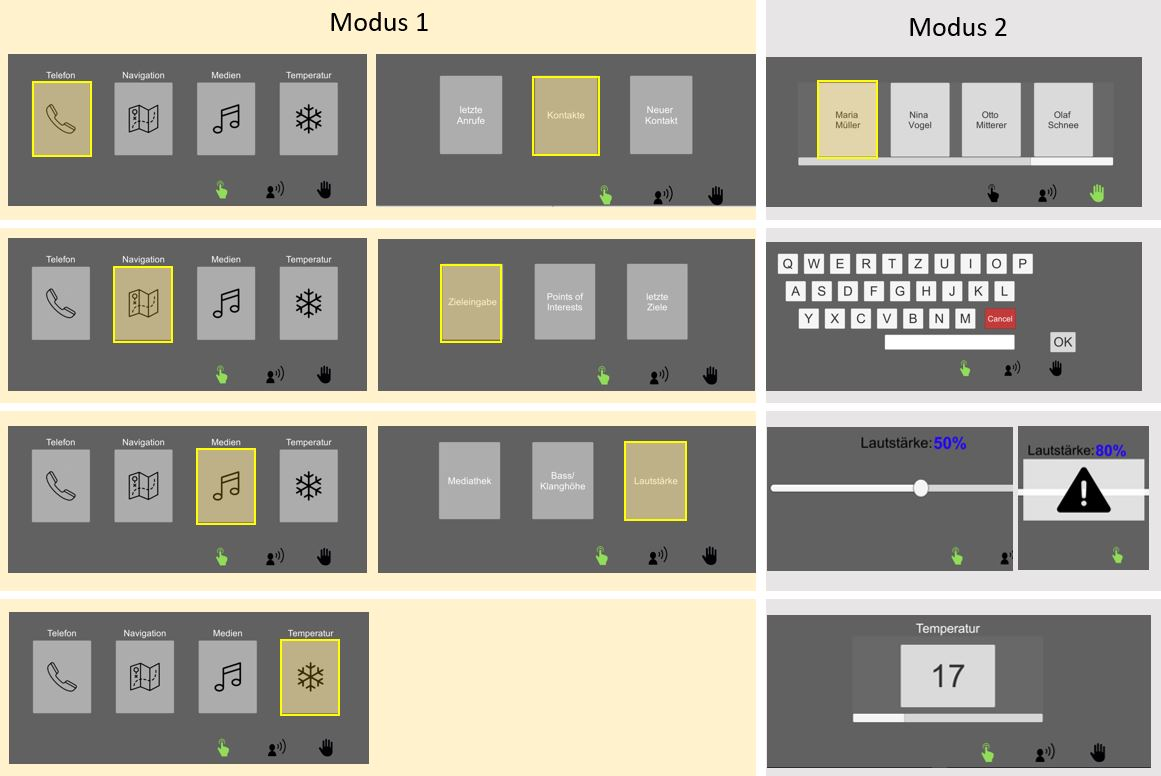
\includegraphics[width=1\textwidth]{img/UseCases2.jpg}
  \caption[Übersicht der Screenabfolge, der 4 Anwendungsbeispiele.]{Übersicht der Screenabfolge, der 4 Anwendungsbeispiele. Ein Anwendungsbeispiel besteht aus den horizontal abgebildeten Screens. Vertikal werden die Anwendungsbeispiele in die erste Modalität und zweite Modalität geteilt. Dazwischen findet der Modalitätswechsel statt. Referenz zu den Icons siehe Kapitel \ref{cha:Danksagung}}
  \label{fig:UseCases}
\end{figure}
Die großen Buttons der ersten beiden Screens, für die Menüstruktur, sowie die Buttons der Liste werden im folgenden Kachel genannt. 
Sie enthalten trotzdem die Funktionalität von Buttons. 

Im ersten Anwendungsbeispiel soll "`Maria Müller"' angerufen werden. Dafür muss im Hauptmenü die Kachel "`Telefon"' auf der linken Seite ausgewählt werden. 
Sobald diese Kachel aktiviert wurde, wechselt der Screen in ein Untermenü mit drei Optionen, von denen die Kachel Kontakte auszuwählen ist. 
Jetzt muss durch eine horizontale Liste von Kontakten navigiert werden. 
Die Liste lässt sich seitenweise scrollen. 
Auf der dritten Seite befindet sich auf der linken Kachel der gewünschte Kontakt "`Maria Müller"', der auszuwählen ist. 
Dieses Anwendungsbeispiel besteht aus einer zweifachen Direktauswahl aus sichtbaren Elementen, einer Listennavigation bestehend aus drei Swipes gefolgt von einer Direktauswahl aus sichtbaren Elementen. 
Die Aktionen sind:
$$\textbf{2* \text{DA} + 3 * \text{L} + \text{DA}}$$

In der zweiten Anwendung soll zu einem von drei verschiedenen Zielen navigiert werden. 
Dazu wird im Hauptmenü die Navigationskachel ausgewählt und anschließend im nächsten Untermenü die Kachel Zieleingabe. 
Um das Ziel einzugeben ist eine vereinfachte Tastatur abgebildet, die per Touch-Eingabe verwendet werden kann. 
Mit dem "`OK"' Button soll die Zieleingabe bestätigt werden. 
Hier bestehen die Aktionen aus zwei Direktauswahlen aus sichtbaren Elementen, einer Texteingabe und der Bestätigung. 
Die Aktionen sind:
$$\textbf{2 * \text{DA} + \text{Xmal Buchst.} + \text{B}}$$

In der dritten Anwendung soll die Lautstärke von 50\% auf 80\% erhöht werden. 
Dazu wird im Hauptmenü die Kachel "`Medien"' selektiert. 
Im darauf folgenden Untermenü ist die Kachel "`Lautstärke"' auszuwählen. 
Die Lautstärke muss mit einem horizontalen Slider auf einen Wert zwischen 75\% und 85\% gestellt werden. 
Dann erscheint eine Warnung als Popup, dass bestätigt werden muss. 
Auch hier setzt sich die Interaktion aus einer zweimaligen Direktauswahl aus sichtbaren Elementen, einer direkten Inkrementation des Sliders und einer Bestätigung zusammen.
Die Aktionen sind:
$$\textbf{2 * \text{DA} + \text{Inkr. (d)} + \text{B}}$$

Das letzte Anwendungsbeispiel hat zum Ziel die Temperatur von 17 auf 20 Grad zu erhöhen. 
Dazu muss im Hauptmenü die Kachel "`Temperatur"' selektiert werden. 
Die aktuelle Temperatur wird angezeigt und kann durch schrittweise Inkrementation einer horizontalen Liste erhöht werden.
Es ist jeweils nur ein Element der Liste, das heißt eine Temperatur, sichtbar.
Dieses Anwendungsbeispiel ergibt sich aus einer Direktauswahl aus sichtbaren Elementen und einer dreifachen Inkrementation des Wertes. 
Die Aktionen sind:
$$\textbf{\text{DA} + 3 * \text{Inkr. (s)}}$$

Das Anwendungsbeispiel "`Einen Song aus einer Liste auszuwählen"' wurde nicht umgesetzt, da ein weiteres  Anwendungsbeispiele die Studiendauer deutlich erhöht hätte. 
Außerdem ähnelt diese Interaktion sehr dem Anwendungsbeispiel einen Kontakt aus einem Liste zu wählen und hätte somit keinen wesentlichen Mehrwert. 
Wir werden dieses Anwendungsbeispiel für die Evaluation verwenden.

Die Direktauswahl aus sichtbaren Elementen wurde immer als erste Modalität verwendet.
Anschließend folgt ein Modalitätswechsel. 
Die drei möglichen Modalitäten wurden mit kleinen schwarzen Symbolen für Touch, Sprache und Geste in jedem Screen angezeigt. 
Die Modalität, die der Proband verwenden soll, wurde grün hervorgehoben. 
In \fref{fig:ModusAktiv} soll beispielsweise mit der Modalität Touch interagiert werden. 
\begin{figure}[ht]
  \centering
  
\includegraphics[width=0.5\textwidth]{img/ModusAktiv.jpg}
  \caption[Symbolische Anzeige der aktiven Modalität]{Symbolische Anzeige der aktiven Modalität, die von den Probanden ausgeführt werden soll. Diese Symbole sind in jedem Screen eingebaut und dienen als Hilfe, welche Modalität verwendet werden soll.
	Referenz zu den Icons siehe Kapitel \ref{cha:Danksagung}}
  \label{fig:ModusAktiv}
\end{figure}

Ist die Modalität Geste aktiv, haben wir eine zusätzliche Information in die Gestensymbolik eingebaut. 
In der aktiven grünen Hand ist ein Punkt zu sehen, der wie bei einer Ampel entweder rot, gelb oder grün ist. 
Dieser Punkt dient dazu besser erkennen zu können, ob und wo die rechte Hand vom Leap Motion Controller erkannt wird. 
Wie in \fref{fig:Ampeldarstellung} zu sehen ist, ist der Punkt rot, wenn die Hand von dem Controller nicht erkannt wird. 
Wird die Hand vom Controller erkannt, befindet sich aber nicht im Interaktionsbereich, indem Gesten ausgeführt werden können, ist der Punkt gelb.
Grün wird der Punkt, sobald die Hand erkannt wurde und sich im Interaktionsbereich befindet.
\begin{figure}[ht]
  \centering
  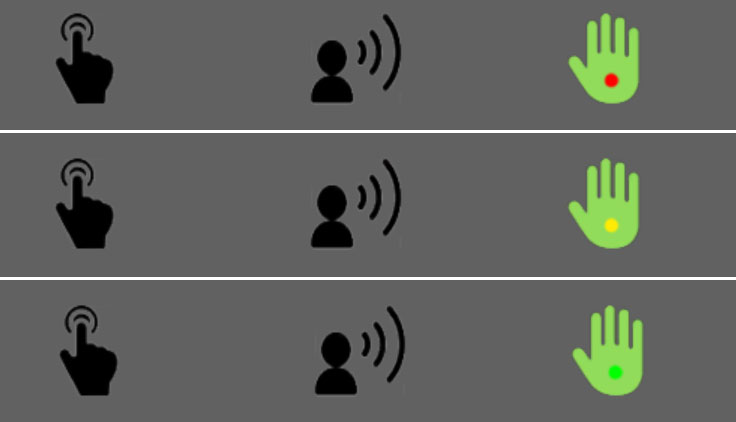
\includegraphics[width=0.5\textwidth]{img/Gestenerkennung.jpg}
  \caption[Ampeldarstellung zur Gestenerkennung]{Ampeldarstellung zur Gestenerkennung. Der rote Punkt bedeutet, das die rechte Hand vom Leap Motion Controller nicht erkannt wurde. 
	Gelb wird der Punkt, wenn die Hand erkannt wurde, sich aber nicht im Interaktionsbereich befindet. 
	Grün ist der Punkt wenn sich die Hand im Interaktionsbereich befindet. Referenz zu den Icons siehe Kapitel \ref{cha:Danksagung}}
  \label{fig:Ampeldarstellung}
\end{figure} 
Mit dieser Visualisierung soll für den Beobachter veranschaulicht werden, falls Gesten nicht erkannt wurden. 

Wird ein Button angewählt bekommt dieser eine gelbe Markierungsfarbe. 
Bei einer Selektion bekommt der Nutzer ein zusätzliches Audio Feedback eines Klickgeräuschs.

\section[Implementation]{Implementation des multimodalen Prototypen}
Der multimodale Prototyp wurde in Unity (Version 5.4 \citep{Unity}) auf einem Surface umgesetzt, was die Touch Interaktion ermöglicht. 
Für die Gestenerkennung wird ein Leap Motionen Controller \citep{Leap} verwendet. 
In Unity wurde ein Software Developer Kit namens Orion \citep{OrionBeta} verwendet, welches in die Unity Szene eingebunden wird. 
Um die Spracherkennung zu gewährleisten wurde in Unity ein Skript eingebunden, dass auf die Windows integrierte Spracherkennung zugreift. 
Die Skripte wurden mit Visual Studio in C\# geschrieben.

Jeder Screen wurde in Unity in eine eigene Szene eingebaut.
Die Selektion eines Buttons durch ein Touch-Event, eine Selektionsgeste oder durch einen Sprachbefehl, lädt die nächste Szene. 
Im ersten Screen wird vom Versuchsleiter die Proband ID eingetragen und die passende Permutation geladen (mehr zur Permutation siehe Kapitel \ref{cha:Studie}). 
In der Permutation steckt das aktuelle Anwendungsbeispiel, sowie die zu verwendenden Modalitäten. 
Die permutierte Reihenfolge der Kombinationen verhindert das eventuell enstandene Lerneffekte unsere Messungen beeinflussen. 

Der Versuchsleiter kann mit den Pfeiltasten einer externen Tastatur das nächste Anwendungsbeispiel laden, einen Messdurchgang aktiviert und den Durchgang gestartet.  
Zur Vorbereitung wird als erstes ein schwarzer Screen für drei Sekunden gezeigt.
Anschließend wird der Hauptscreen geladen, mit dem die Interaktion beginnt.

Um Fehler zu reduzieren ist es mit den Modalitäten Geste und Sprache nicht möglich eine falsche Auswahl zu tätigen. 
Wir haben uns entschieden für die Sprache keinen Push To Talk Button zu verwenden, da wir Aktionszeiten messen wollen und wir uns auf die Modalitäten Touch, Geste und Sprache fokussieren. 
Sollter dieser haptische Knopfdruck verwendet werden, müsste die Zeit für diese Aktion hinzugefügt werden.  

\subsection[Touch]{Realisierung der Toucheingabe} 
\citet{Wobbrock:2009} untersucht von Nutzern definierte Touchgesten auf einem Surface. 
Sie fanden heraus, dass die Anzahl der Finger für eine Touchgeste für die meisten Nutzer irrelevant ist und das einhändige Touchgesten bevorzugt werden. 
Bei unseren Touchgesten entschieden wir uns für drei verschiedene Touchgesten (siehe \fref{fig:TouchGestures}):
\begin{itemize}
\item Einen direkten Touch (Tap), um einen Button auszuwählen. 
Die Selektion geschieht erst wenn der Finger den Touchscreen verlässt. 
\item Eine Swipegeste, um eine Liste seitenweise zu scrollen oder einen Wert zu inkrementieren.
\item Eine direkte Inkrementation des Slides, um den Wert des Sliders zu verstellen (Slidegeste).
Hierbei wird der Regler des Slider ähnlich wie bei Drag and Drop direkt verschoben, allerdings nur entlang des Achse des Sliders.
Der Finger bleibt während der Verschiebung auf der Touchfläche.
\end{itemize}
In der \ref{fig:TouchGestures} sind die 3 Varianten veranschaulicht.
\begin{figure}[ht]
	\centering
		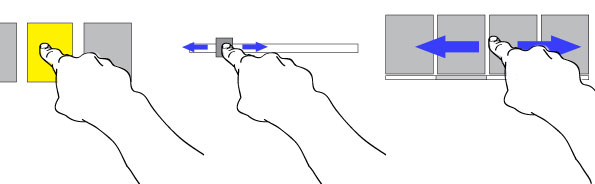
\includegraphics[width=1\textwidth]{img/TouchGestures.jpg}
	\caption{Touchgesten: Tap, Slidegeste und Swipegeste für die Toucheingabe}
	\label{fig:TouchGestures}
\end{figure}

\subsection[Geste]{Realisierung der Gesteneingabe}
Auch bei der Erkennung der Gesten wurden drei verschiedene Arten implementiert. 
Um einen Button zu selektieren wird zuerst geprüft, ob sich eine rechte Hand im festgelegten Interaktionsbereich befindet. 
Dieser Interaktionsbereich ist je nach Anzahl der Buttons in drei oder vier Bereiche entlang der x-Achse unterteilt. 
Je nachdem in welchem Bereich sich die Hand befindet ändert der passende Button dieses Bereichs die Farbe zu gelb.
Dies entspricht der Markierungsfarbe. 
Somit erkennt der Nutzer welcher Button gerade angewählt ist. 
Um einen Button nun zu selektieren, muss der Zeigefinger schnell nach unten bewegt werden, ohne dabei die Hand zu bewegen. 
Nur wenn ein entsprechender Button gelb markiert ist und die Selektionsgeste mit dem Zeigefinger ausgelöst wurde, wird dieser Button selektiert und somit die nächste Szene geladen. 

Die nächste Geste ist eine Wischgeste, um in einer Liste seitenweise zu scrollen oder einen Wert zu inkrementieren.
Das entspricht unseren Aktionen (L) und (Inkr. (s)). 
Diese Geste wurde in den Anwendungsbeispielen verwendet, um die Temperatur zu verändern und um die Liste der Kontakte zu durchsuchen. 
Wie zuvor muss die rechte Hand erkannt werden und sich im Interaktionsbereich befinden. 
Wenn sich die Hand entlang der x-Achse mit mindestens 80 Millimeter pro Sekunde von rechts nach links bewegen, löst dies eine Animation aus, die zur nächsten Seite navigiert. 
Damit die Hand nicht unbeabsichtigt zwei Seiten auf einmal oder direkt hintereinander scrollen lässt, wird die Erkennung der Wischgeste nach jeder Erkennung für eine Sekunde deaktiviert. 

Die dritte und letzte Geste ist eine Geste, um einen Slider zu verstellt. 
Hierfür müssen sich Daumen und Zeigefinger berühren und somit einen geschlossenen Kreis über dem Leap Motion Controller bilden.
Damit dieser Kreis von der Leap erkannt wird, ist es wichtig die anderen Finger abzuspreizen, siehe \ref{fig:Gestures}. 
Ist dieser Kreis geschlossen wird der Slider aufgenommen und kann verschoben werden. 
Um den Slider nach rechts oder links zu verstellen muss die Geste entlang der x-Achse durch Bewegung der Hand in eben diese Richtung verändert werden. 
Ist der gewünschte Wert erreicht, muss der Kreis geöffnet werden, indem sich Zeigefinger und Daumen wieder lösen. 
\begin{figure}[ht]
	\centering
		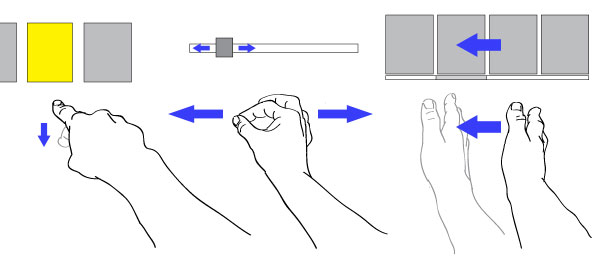
\includegraphics[width=1\textwidth]{img/Gestures-mit_Pfeile.jpg}
	\caption{Selektionsgeste, Slidegeste und Swipegeste}
	\label{fig:Gestures}
\end{figure}

\subsection[Sprache]{Realisierung der Spracheingabe}
Um die Spracherkennung zu ermöglichen wurden in Unity in jeder Szene die dementsprechenden Sprachbefehle als String definiert. 
Im Beispiel des Hauptscreens waren dies die Sprachbefehle: "`Telefon"', "`Navigation"', "`Medien"' und "`Temperatur"'. 
Die in Windows integgriert Spracherkennung verarbeitet gesprochene Befehle zu Strings.
Stimmt Strings mit einem der vordefiniertem String überein wird der passende Button selektiert. 

Damit der Nutzer bei der Direktauswahl aus sichtbaren Elementen zusätzlich zum Soundgeräusch Feedback bekommt wird der selektierte Button vor dem tatsächlichen Klick farblich gelb hervorgehoben. 
Um diesen Effekt erzielen zu können musste eine Verzögerung von einer halben Sekunden eingebaut werden.

Im Beispiel der Listen wird zur Veranschaulichung erst zum entsprechenden Wert geswiped, das heißt eine Animation ist sichtbar und anschließend wird die Kachel selektiert. 
Im Beispiel der Texteingabe wird das Inputfeld mit dem gesprochenen Ziel aktualisiert.

\subsection[Protokollierung]{Protokollierung der relevanten Events}
Um die Interaktionszeiten messen zu können werden die relevanten Aktionen mit Zeitstempeln in einer Textdatei protokolliert (Logdatei). 
Diese Logdatei ist so strukturiert, dass Werte durch Tabs separiert sind, um später in Excel leichter bearbeitet werden zu können.
An relevanten Stellen im Code wird die Logdatei geöffnet und der Zeitstempel zusammen mit dem Event in die Datei geschrieben und wieder geschlossen. 
Zur Veranschaulichung ist in \fref{fig:Auszug_Logging_Sound_TT} ein Auszug des Protokolls zusehen. 
Die Logdatei wurde hier bereits angepasst und in Excel als Tabelle formatiert (mehr dazu in Kapitel \ref{cha:Studie}). 
\begin{figure}[ht]
	\centering
		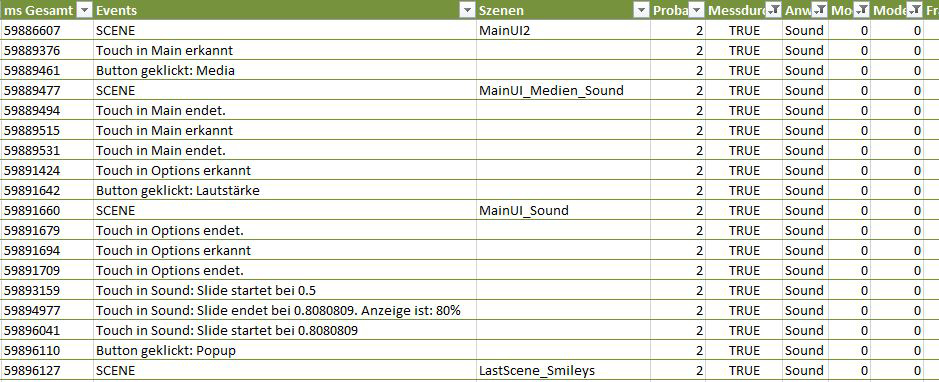
\includegraphics[width=1\textwidth]{img/Auszug_Logging_Sound_TT.JPG}
	\caption[Ausschnitt aus der Logdatei vom Anwendungsbeipiel Lautstärke]{Ausschnitt aus der Logdatei vom Anwendungsbeipiel Lautstärke, das mit den Modalität Touch und Touch, also unimodal ausgeführt wurde}
	\label{fig:Auszug_Logging_Sound_TT}
\end{figure}

Sobald ein Anwendungsbeispiel startet werden die Einstellungsinformationen siehe \fref{fig:ProbandenSettings} protokolliert. 
Diese enthalten die ID des Probanden, das aktuelle Anwendungsbeispiel, die zu verwendenden Modalitäten und ob es sich um einen Probe- oder um einen Messdurchgang handelt. 
Nach jedem Messdurchgang werden die Antworten protokolliert, die die Probanden über Eignung und Gefallen der gerade ausgeführten Moduskombination eingaben. TODO(smileys erwähnen bzw. Erläuterung hier einbauen)
Nach jedem Durchgang erscheint wieder der Einstellungsscreen, indem der Versuchsleiter das nächste Anwendungsbeispiel laden oder den Messdurchgang aktiviert kann. 
Für jede Runde werden die entsprechenden Infos vom Setting protokolliert.
\begin{figure}[ht]
  \centering
  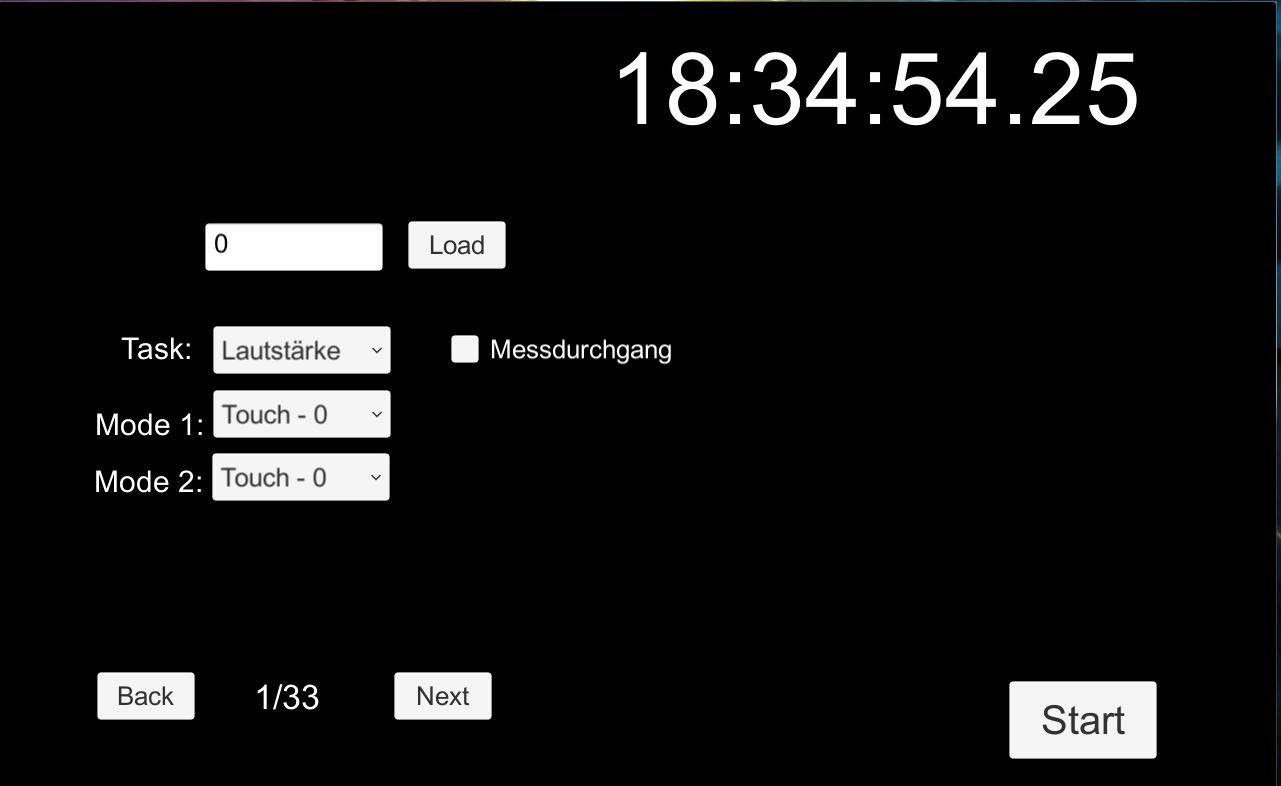
\includegraphics[width=1\textwidth]{img/SettingsPrototyp.jpg}
  \caption{Einstellungen vor jedem Durchlauf}
  \label{fig:ProbandenSettings}
\end{figure} 

Während des Anwendungsbeispiels wird der aktuelle Screen protokolliert, sobald er sichtbar geladen wurde. 
Jeder Touch, jede erkannte Geste und jeder erkannte Sprachbefehl wird ebenfalls protokolliert. 
Außerdem wird bei Listen die aktuelle Seite und beim Slider die Start- und Endwerte während einer Bewegung durch Touch oder Geste protokolliert. 
Bei jedem Button wird der Name des Buttons protokolliert, sobald der Button ausgelöst wurde. 
Mit diesen Logzeiten sollen nach der Studie die Zeiten der Operatoren berechnet werden. 
Dazu mehr in Kapitel \ref{cha:Studie}.  


\chapter[Studie und Auswertung]{Studie zur Erhebung multimodaler Interaktionszeiten und Auswertung}\label{cha:Studie}
In diesem Kapitel wird das Studiendesign und die Durchführung der Studie beschrieben, sowie auf die anschließende Auswertung eingegangen.

\section[Studiendesign]{Studiendesign zur Erhebung multimodaler Interaktionszeiten}
Für die Studie verwenden wir ein within-subject Design, bei dem jeder Proband alle Kombinationen der vier Anwendungsbeispiele im stehenden Auto durchführen soll.

\subsection[Permutation]{Permutation der Anwendungsbeispiele}
Jedes Anwendungsbeispiel verfügt über eine Moduswechsel.
Durch die drei verschiedenen Modalitäten (Touch, Gestik und Sprache) kommen wir somit auf auf neun Kombinationen pro Anwendungsbeispiel. 
Eine Ausnahme ist das Navigationsanwendungsbeispiel, bei dem wir uns entschieden haben die Zieleingabe nicht für die Gestik umzusetzen. 
Somit fallen die Varianten Geste \& Geste, Sprache \& Geste und Touch \& Geste weg. 
Damit kommen wir bei diesem Anwendungsbeispiel lediglich auf sechs multimodale Kombinationen. 
Zu den multimodalen Varianten testen wir auch die drei unimodalen Varianten der vier Anwendungsbeispiele und kommen insgesamt auf ($9*4-3=$) 33 Varianten für alle vier Anwendungsbeispiele, die jeder Proband durchzuführen hat. 
\begin{figure}[ht]
  \centering
  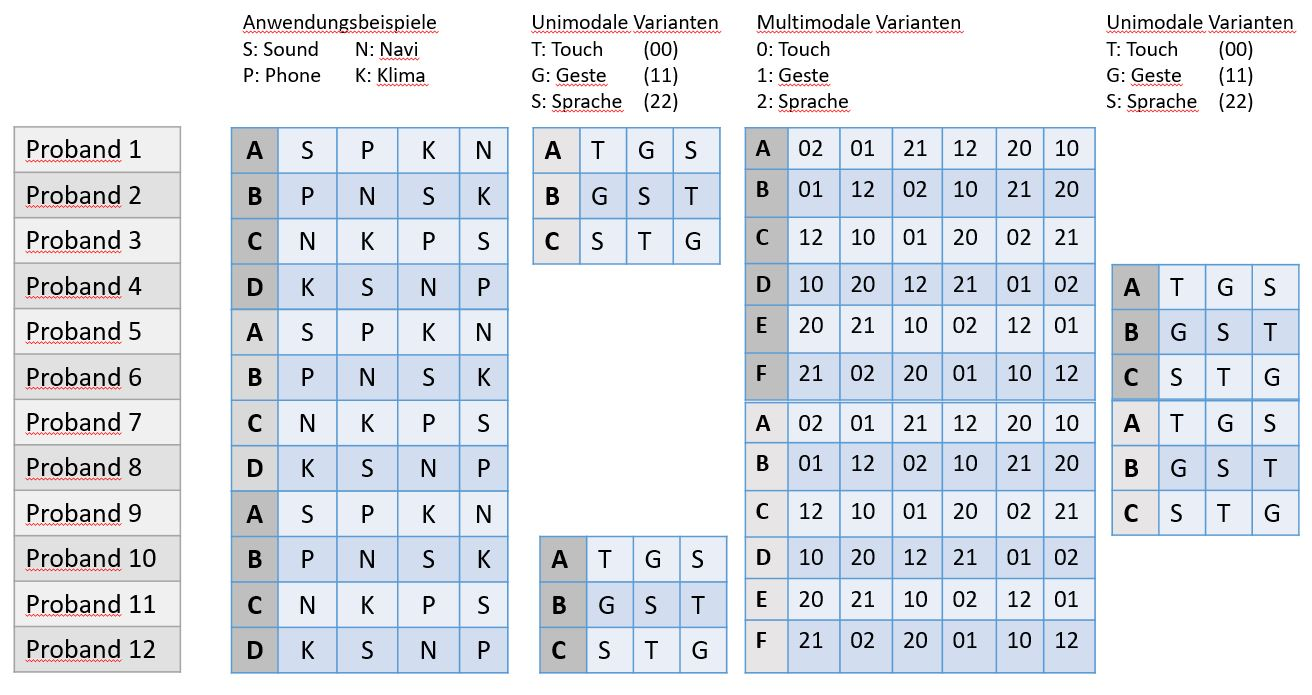
\includegraphics[width=1\textwidth]{img/Permutation.jpg}
  \caption[Permutation der Anwendungsbeispiel]{Permutation der Anwendungsbeispiel, der unimodalen Varianten und der multimodalen Varianten pro zwölf Probanden}
  \label{fig:Permutation}
\end{figure} 

Um Lerneffekte zu vermeiden wurden die vier Anwendungsbeispiele mittels Balanced Latin Square permutiert (vier Permutationen).
Die drei unimodalen Kombinationen wurden mittels Latin Square permutiert (drei Permutationen) und die sechs multimodalen Kombinationen erneut mittels Balanced Latin Square (sechs Permutationen).
Die Permutation der Modalitäten wurde für jeden Proband fixiert, das heißt für jedes Anwendungsbeispiel gleich angewendet. 

Bei zwölf Probanden ist es möglich die vier verschiedenen Permutationen der Anwendungsbeispiele drei mal zu wiederholen. 
Die drei unimodalen Kombinationen werden vier mal wiederholt und die sechs Permutationen der multimodalen Kombinationen werden zwei mal innerhalb von zwölf Probanden wiederholt. 
Zudem wird die Reihenfolge von unimodalen und multimodalen alterniert (siehe \fref{fig:Permutation}). 
Dieses Vorgehen wird für die nächsten zwölf Probanden wiederholt. 
Die drei verschiedenen Zieleingaben werden ebenfalls mit dem Latin Square permutiert und auf die permutierte Moduskombination verteilt. 
Mit diesen Vorkehrungen können wir davon ausgehen, dass mögliche Lerneffekte gleich verteilt sind.

\subsection[Fragebögen]{Fragebögen der Studie}
Es wurden zwei verschiedene Fragebögen erstellt (siehe Kapitel \ref{cha:Anhang}). 
Im ersten Fragebogen werden demografischen Angaben wie Name, Alter, Händigkeit und die Muttersprache abgefragt, sowie die bereits gesammelten Erfahrungen im Umgang mit Interaktionen durch Touch, Geste und Sprache. 
Auf die Frage der Nutzungshäufigkeit wurden vier Antwortmöglichkeiten unterschieden:
\begin{itemize}
	\item ja, benutze ich regelmäßig 
	\item ja, benutze ich gelegentlich
	\item ja, aber nur sehr wenig
	\item nein
\end{itemize}



Der zweite Fragebogen wird nach der Durchführung der Studie ausgefüllt. 
Darin wird abgefragt, wie geeignet die Modalitäten für die verschiedenen Screentypen sind. 
Dies wird mit einer Likertskala mit fünf Auswahlmöglichkeiten für jede Modalität abgefragt.  
Die Auswahlmöglichkeiten gehen von nicht geeignet bis geeignet. 
Außerdem wird ein Ranking für die verschiedenen Screentypen abgefragt, indem sich der Proband entscheiden muss welcher Modus für die unterschiedlichen Screentypen am besten, zweitbesten und am schlechtesten geeignet ist.  

Die kompletten Fragebögen, Einverständniserklärung, sowie der Studienleitfaden sind am Ende dieser Arbeit angehängt (siehe Kapitel \ref{cha:Anhang}).

\section{Durchführung der Studie}
Die Studie fand in Garching-Hochbrück in der Parkgarage von BMW in einem 6er Gran Coupé statt. 
Die Studiendauer betrug circa 1,5 Stunden. 
Das Auto wurde ans Stromnetz angeschlossen, um das Surface zu laden und eine Dauerhafte Stromversorgung für Licht sowie Sitzheizung zu ermöglichen.

Pro Tag konnten bis zu vier Probanden an der Studie teilnehmen. 
Bevor der erste Durchgang begann wurde der Akku der GoPro Kamera ausgetauscht und eine leere Speicherkarte eingelegt. 
Im Kofferraum konnten Ersatzbatterien für die Kamera geladen werden. 
Nach jedem Probanden wurde der Akku gewechselt und der gebrauchte erneut geladen. 
Die Speicherkarten von 32GB wurden nach jedem zweiten Probanden gewechselt und anschließend auf eine Festplatte kopiert. 
Die Kamera wurde mittig, zwischen Fahrer und Beifahrer an der Decke befestigt und Richtung Surface ausgerichtet (siehe \fref{fig:Kamera}).
\begin{figure}[ht]
  \centering
  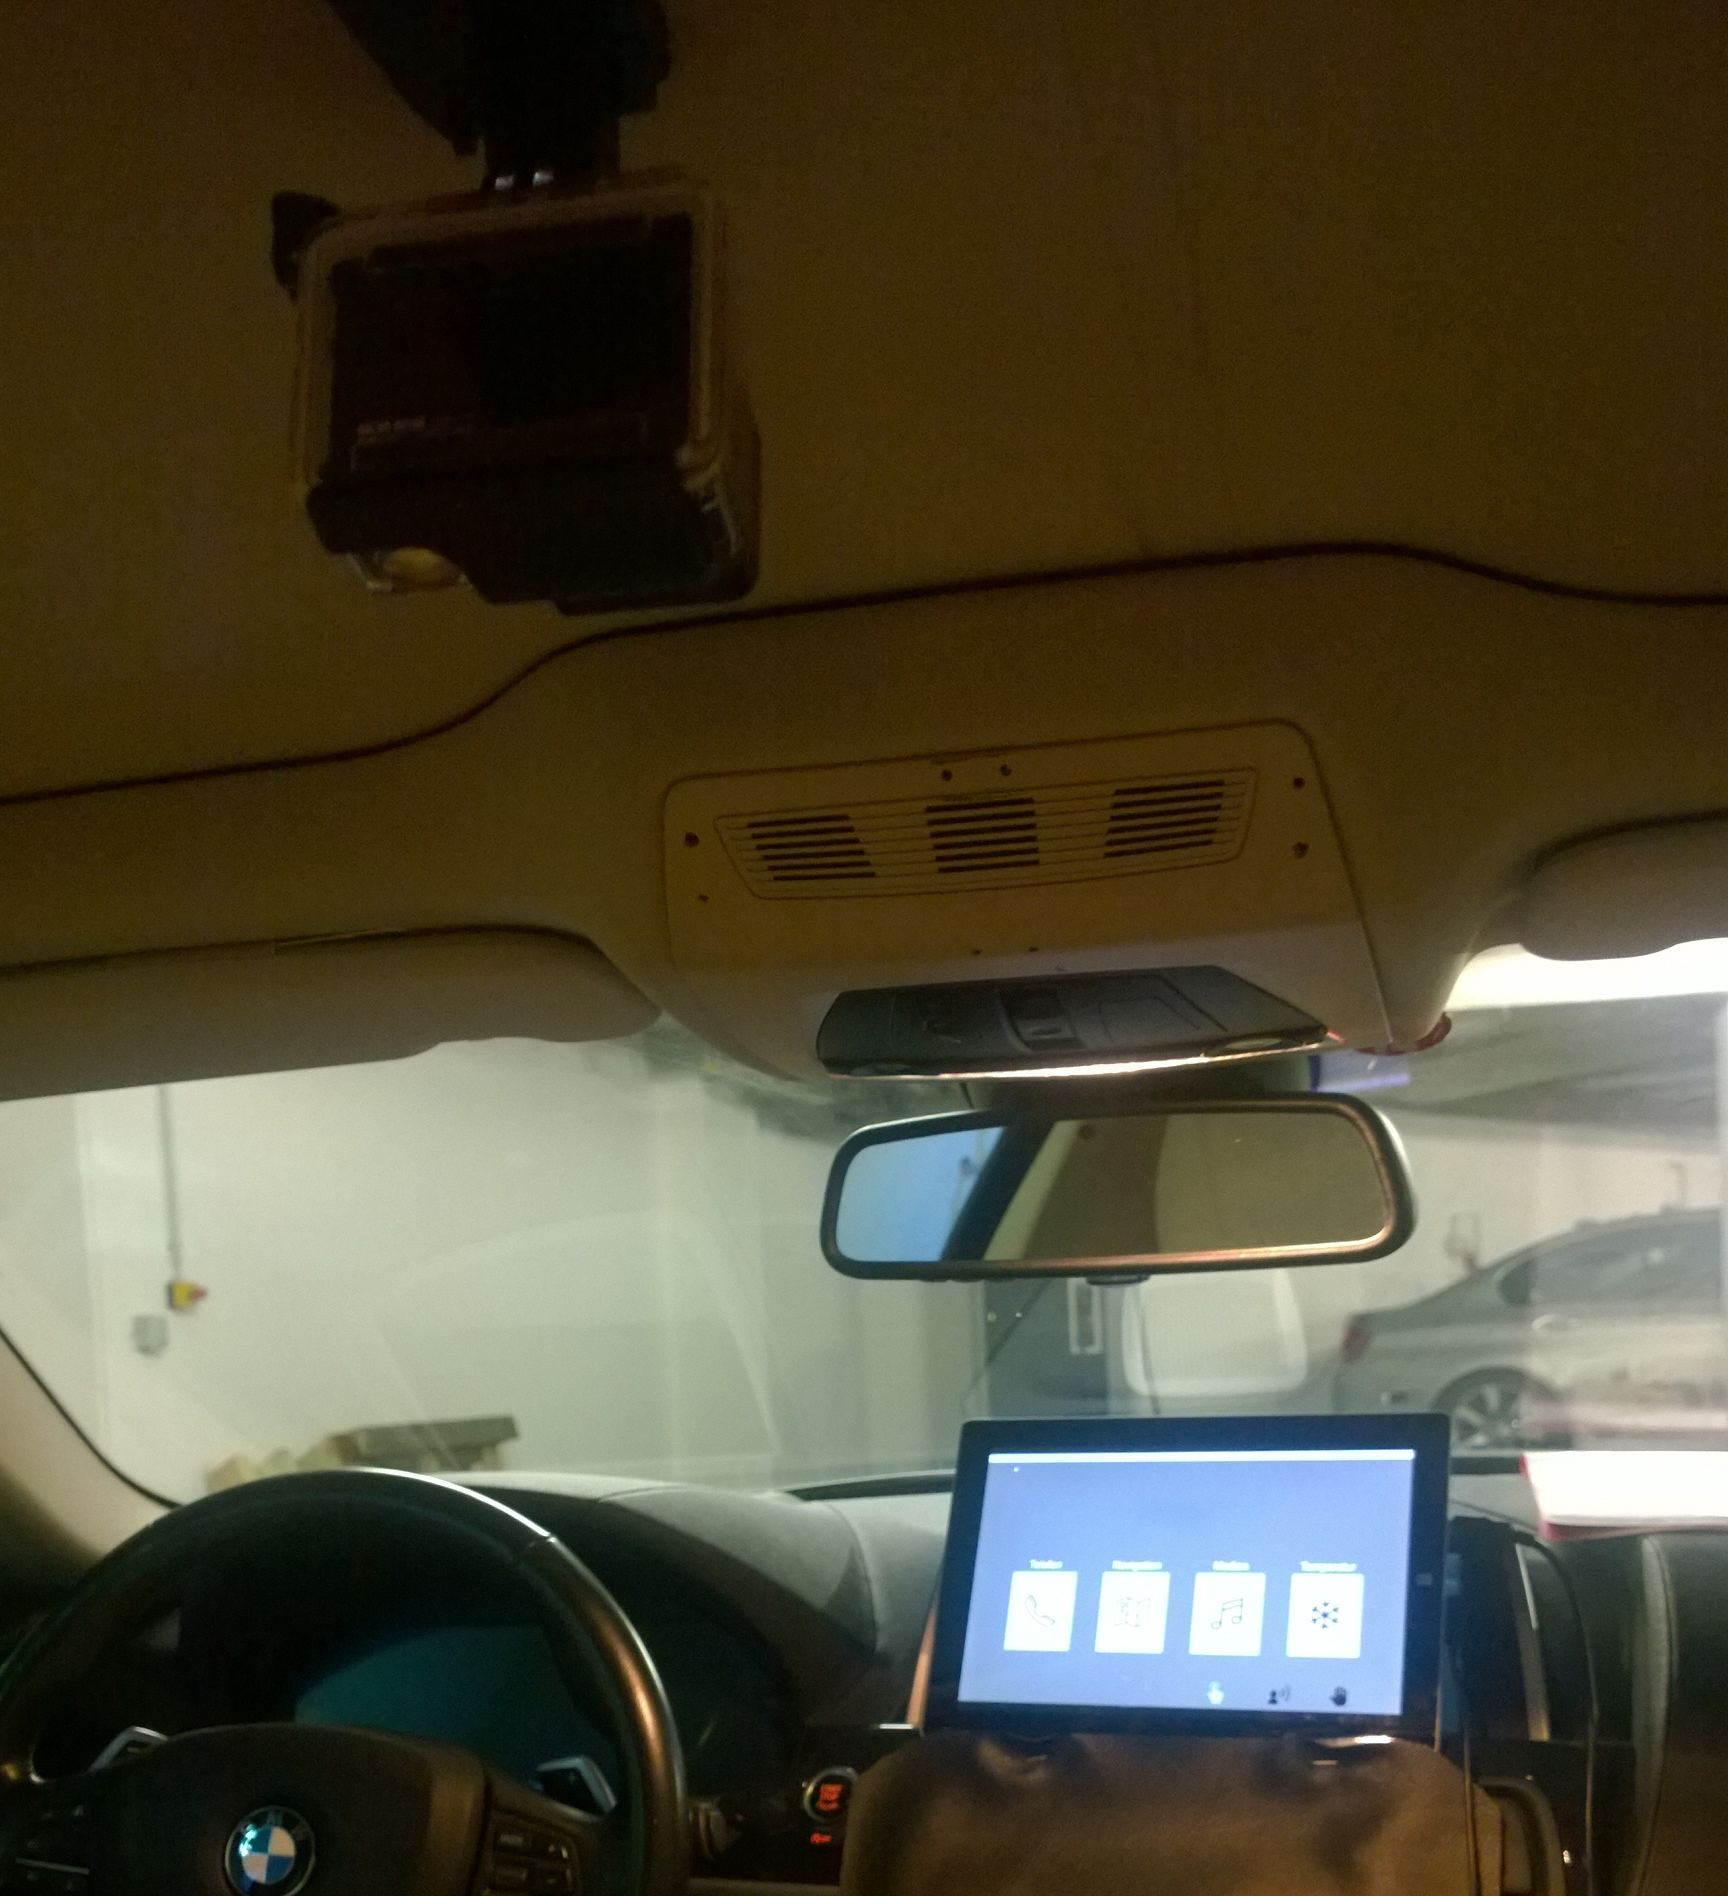
\includegraphics[width=0.5\textwidth]{img/Kamera3.jpg}
  \caption{Anbringung der Kamera im Studienauto}
  \label{fig:Kamera}
\end{figure} 

Jeder Proband wurde am Empfang am Parkrings 19 abgeholt und begrüßt.
Es wurde darauf hingewiesen, dass die Studie bis zu 1,5 Stunden dauern wird und das jetzt die beste Gelegenheit wäre, um wenn nötig noch auf die Toilette zu gehen.
Anschließend begaben wir uns in die Parkgarage zum Testfahrzeug, indem der Proband auf dem Fahrersitz platz nehmen sollte, während der Studienleiter am Beifahrersitz platz nahm.
Der Proband wurde darauf hingewiesen seinen Sitz einzustellen, als würde er oder sie das Auto fahren.

Nachdem sichergestellt wurde, dass alle Smartphones auf lautlos gestellt sind, wurde das Thema kurz erläutert und darauf aufmerksam gemacht, dass zur Erhebung der Interaktionszeiten verschiedene Daten protokolliert werden und zusätzlich die Studie mit einer GoPro aufgezeichnet wird.
Darüber aufgeklärt musste jeder Proband eine Einverständniserklärung unterschreiben (siehe Kapitel \ref{cha:Anhang}).
Zusätzlich sollte ein kurzer Fragebogen zu demografischen Daten und den Vorerfahrungen zum Umgang mit den Interaktionen Touch, Geste und Sprache ausgefüllt werden.
In der Zwischenzeit startete der Studienleiter das Programm, stellte die richtige ID ein und überprüfte die neu geladene Permutation.

Jetzt wurde das Vorgehen der Studie anhand des ersten Anwendungsbeispiel mit Hilfe der ausgedruckten Übersicht der Anwendungsbeispiele \ref{fig:UseCases} erläutert.
Sobald das erste Anwendungsbeispiel und die Vorgehensweise klar war, wurde die GoPro gestartet und der Proband konnte mit dem ersten Probedurchlauf beginnen. Dazu hatte der Proband seine Hände am Lenkrad und der Studienleiter startete die Anwendung mittels einer externen Tastatur. 
Der Screen wird nach dem Start zuerst für drei Sekunden schwarz bis dann der Hauptscreen zu sehen ist und die Interaktion beginnen kann.
Insgesamt wurden 33 verschiedene Durchläufe von jedem Proband getestet.
Zu jedem dieser Varianten, bestehend aus den vier Anwendungsbeispielen und deren Kombinationen von Modalitäten, sollte mindestens ein Probedurchlauf gemacht werden.

Der Probedurchlauf diente dazu den Probanden mit der Aufgabe vertraut zu machen und sich an die möglicherweise neue Interaktionsmethode zu gewöhnen.
Die Probedurchläufe wurden so oft wiederholt, bis die Aufgabe klar verstanden und fehlerfrei ausgeführt wurde. 

Nach dem Probedurchlauf wurden zwei Messdurchgänge durchgeführt, die für die Erhebung der Interaktionszeiten verwendet werden.
Da wir nur fehlerfreie Messdurchgänge benötigen, wurde im Falle eines Fehlers in einem Messdurchgang, dieser wiederholt.
Passierte dies kennzeichnete der Studienleiter dies in seinen Notizen zu dieser Variante, um später nur die gültigen Messdurchgänge zu verwenden.
Auch interessante Anmerkungen oder Auffälligkeiten wurden während der Studie notiert.

Nach den mindestens 99 Durchgängen $((1 * \text{Probedurchgang} + 2 * \text{Messdurchgänge}) * 33 \text{Varianten})$ konnte die Kamera gestoppt werden und die Probanden sollten den anschließenden Fragebogen ausfüllen.
Währenddessen konnten Anmerkungen vom Versuchsleiter notiert werden. 
Als Dankeschön bekamen die Probanden nach der Studie Schokolade.

Nach jedem Studiendurchgang wurde der Akku der Kamera gewechselt. Die Speicherkarte wurde nach jedem zweiten Probanden gewechselt.

\section[Quantitative Auswertung]{Quantitative Auswertung der Studienergebnisse}
Im Folgenden werden die quantitativen Ergebnisse der Studie präsentiert.
In einem Zeitraum von zwei Wochen nahmen insgesamt 22 Probanden an der Studie zur Erhebung der Interaktionszeiten teil.
hierbei wurden über 22 Stunden Videomaterial aufgezeichnet. 
\subsection[Studienteilnehmer]{Studienteilnehmer}
Das Alter der 22 Studienteilnehmer (14 männlich und 8 weiblich) beträgt im Durchschnitt $30,55$ Jahre. 
Der Altersbereich erstreckt sich von 22 bis 58 Jahren. 
Mode und Median ergaben je 25 Jahre. Neun der 22 Probanden sind rechtshändig, zwei linkshändig und ein Proband gab an beidhändig zu sein. 
Alle Teilnehmer sprechen deutsch als Muttersprache.

Die Vorerfahrungen mit der Bedienung von Touch, Gesten und Sprache der Teilnehmer wurde von den Probanden als Selbsteinschätzung abgefragt. 
Auf die Frage, ob sie Erfahrung mit der Bedienung von Sprache, Touch und Geste haben, konnte aus vier Optionen gewählt werden (1: nein, 2: ja, aber nur sehr wenig, 3: ja, benutze ich gelegentlich und 4: ja, benutze ich regelmäßig). 

Die Vorerfahrung von Sprache ergab im Durchschnitt $2,32$, bei Touch $3,95$ und bei Geste $1,86$. Die genauen Angaben der Probanden können aus \fref{fig:Vorerfahrung} entnommen werden.
\begin{figure}[ht]
  \centering
  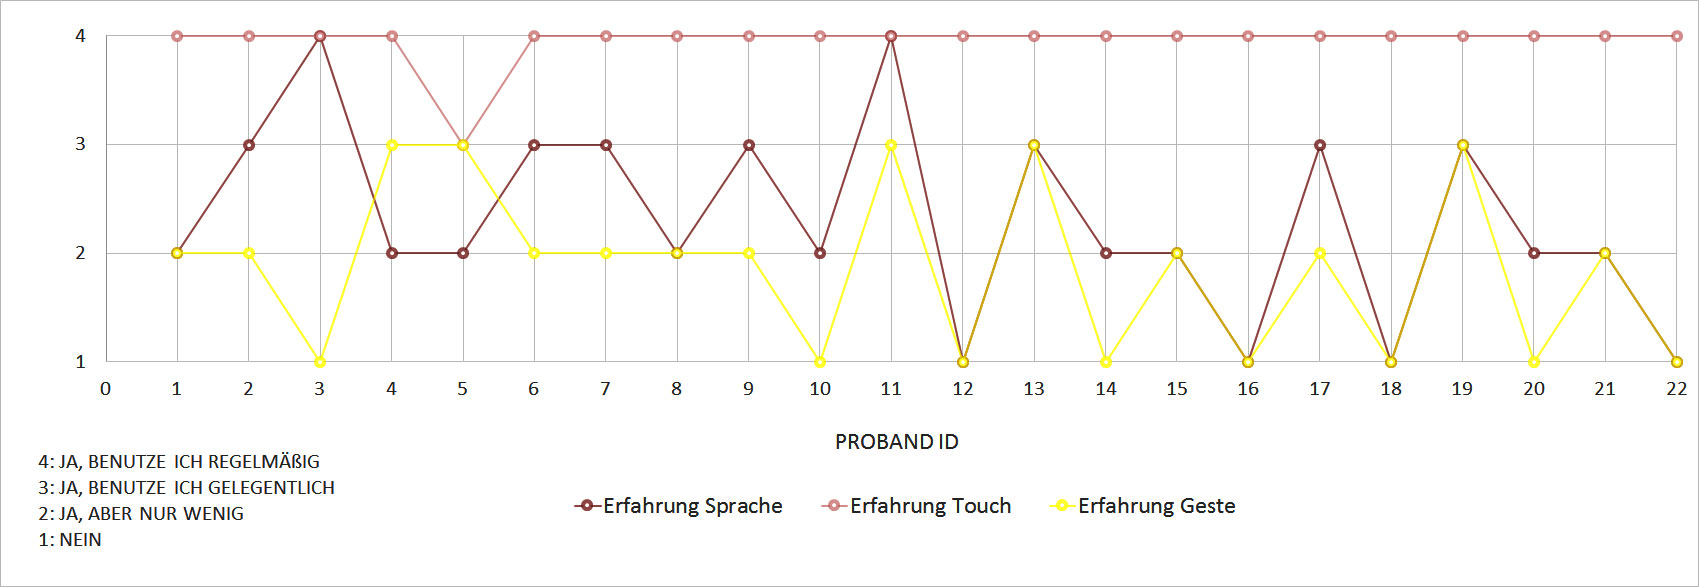
\includegraphics[width=1\textwidth]{img/ErfahrungProbanden2.jpg}
  \caption[Vorerfahrung der Probanden]{Vorerfahrung der Probanden mit der Bedienung von Touch, Sprache und Geste. Einschätzung der Probanden auf die Frage: Haben Sie Erfahrung bei der Bedienung von Sprach-, Touch- und Gestensteuerung.}
  \label{fig:Vorerfahrung}
\end{figure}

\subsection[User Experience]{User Experience}
Nach jedem Messdurchgang wurden die Nutzer gefragt wie geeignet sie diese Interaktion fanden und ob sie Ihnen gefallen hat. 
Wie bei einer Likert-Skala werden 5 Antwortoptionen unterschieden. Zwei negative, eine neutrale und zwei positive (siehe \fref{fig:Uebersicht_Eignung}). 
Aus den Antworten ist deutlich zu sehen, dass die unimodale Variante mit Sprache in beiden Bereichen stets am besten abschnitt. 
Die Unterschiede zwischen Eignung und Gefallen sind nicht sehr groß, allerdings fällt auf, dass vor allem die Interaktionen mit Geste den Nutzern besser gefällt als sie deren Eignung einschätzen. 
Am zweit beliebtesten in beiden Kategorien war die Kombination von Touch und Sprache. 
Bei dem Anwendungsbeispiel Lautstärke war die Kombination Touch und Sprache sogar in Eignung und Gefallen noch etwas besser als die unimodale Sprachvariante. 
Die dritt beliebteste Variante im Anwendungsbeispiel Lautstärke war die Kombination Sprache und Touch. 
Bei allen anderen Anwendungsbeispielen war die dritt beliebteste Kombination Geste und Sprache. 

Die Geste hat bei der Direktauswahl die besten Ergebnisse verglichen zu den anderen Operatoren. 
Ein sehr eindeutiges Ergebnis aus den Fragebögen bekommen wir bei der Texteingabe, für die Sprache eindeutig besser geeignet ist, als per Touch das gewünschte Ziel einzutippen siehe \fref{fig:Uebersicht_Eignung}.
\begin{figure}[ht]
  \centering
  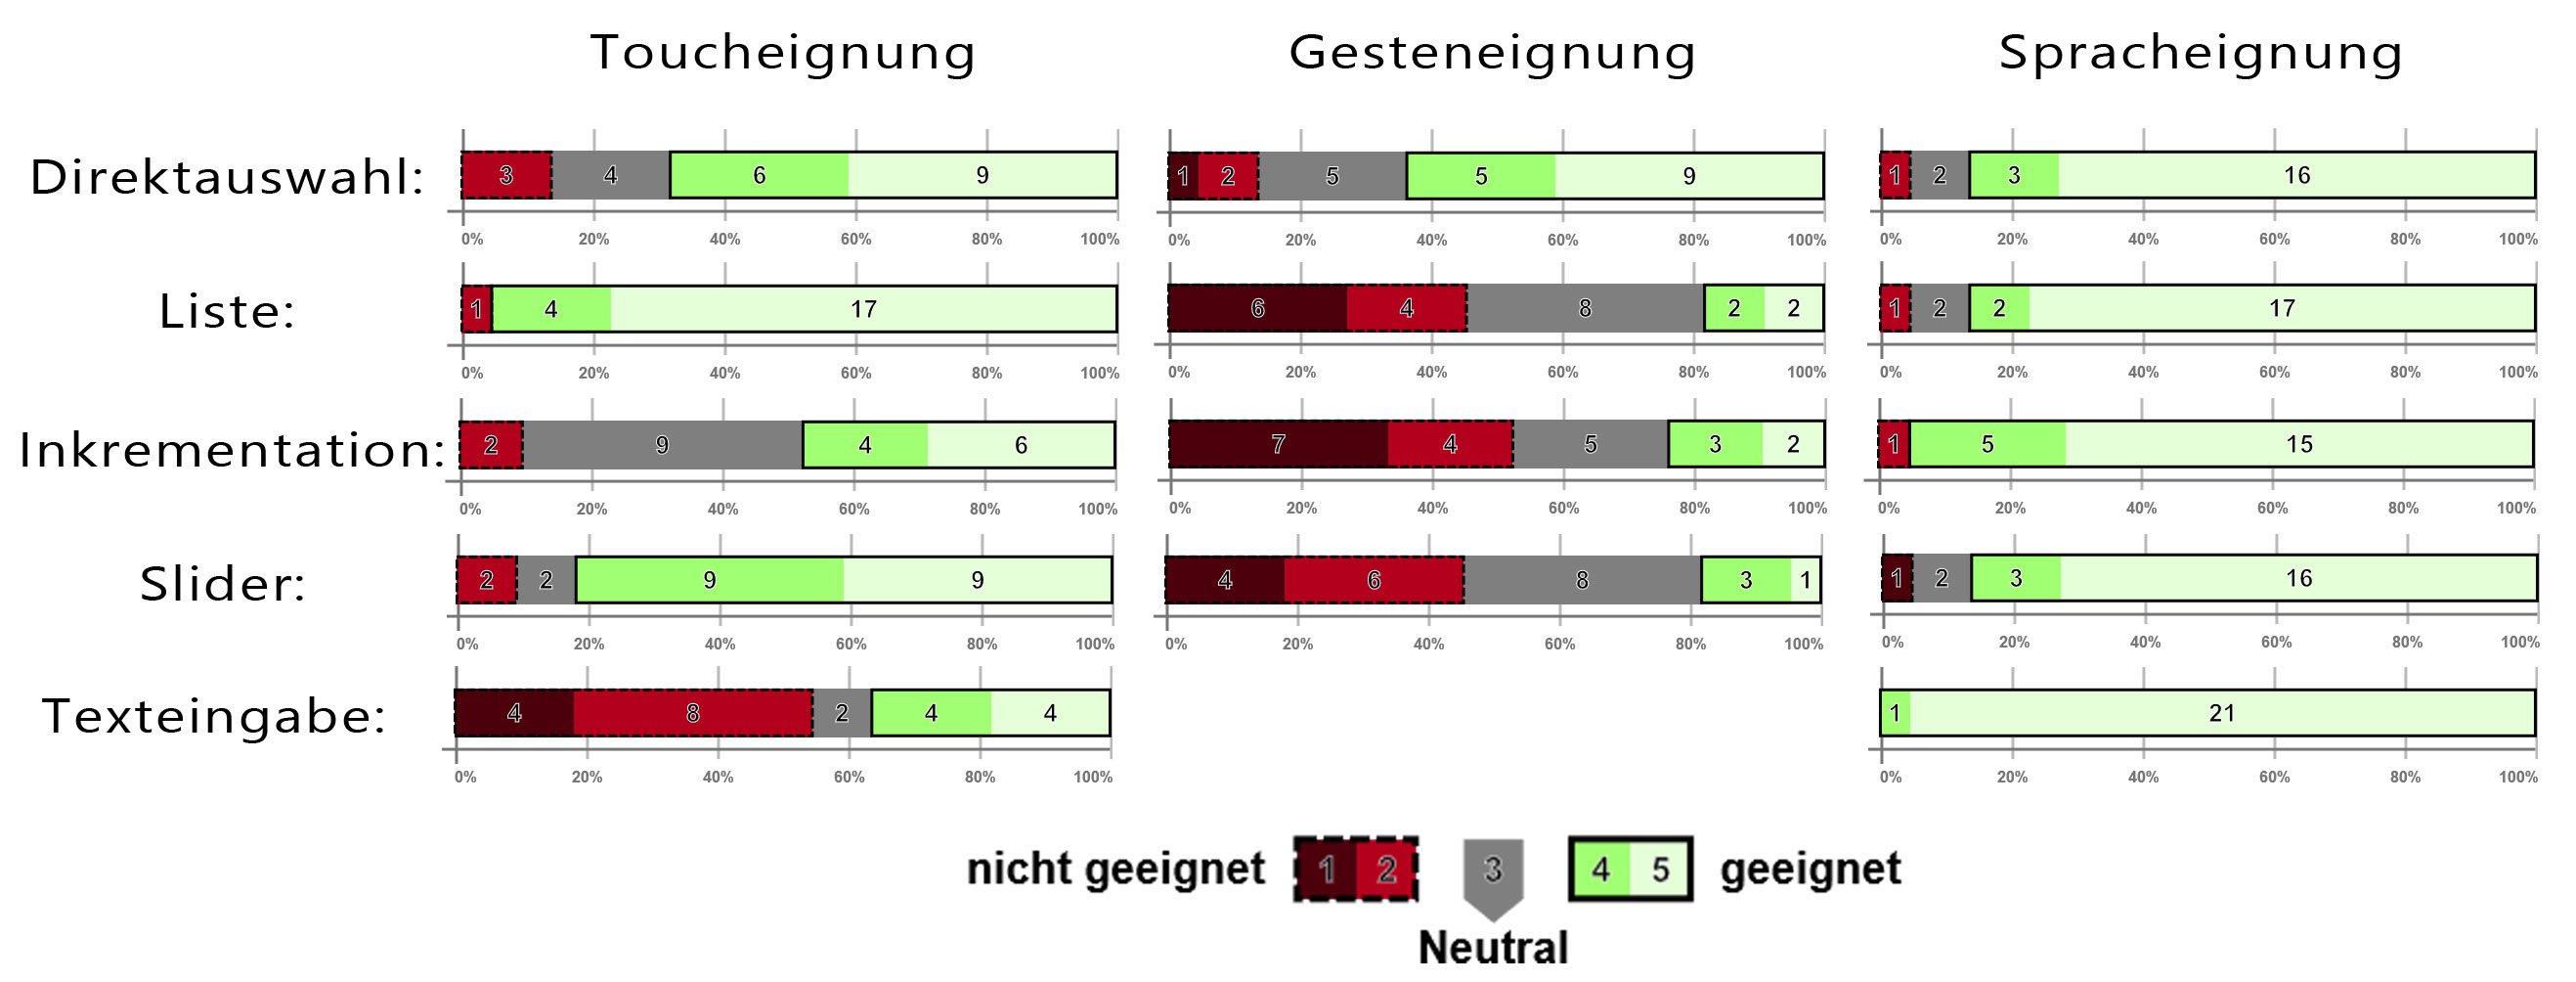
\includegraphics[width=1\textwidth]{img/Uebersicht_Eignung}
  \caption[Eignung des Screentypen]{Einschätzung der Probanden, wie geeignet Sie die verschiedenen Screentypen für die jeweilige Modalität halten. 
	Die Balkendiagramme zur Darstellung von Likert-Skalen wurde mit http://likertplot.com/ generiert.}
  \label{fig:Uebersicht_Eignung}
\end{figure}

Im zweiten Teil des Fragebogen sollten die Screentypen noch mit einem Ranking versehen werden. 
Hierbei mussten sich die Probanden entscheiden welche Modalität am besten, zweitbesten und am schlechtesten geeignet ist. 
Bei der Direktauswahl aus sichtbaren Elementen halten 10 von 22 die Touch-Eingabe, 8 die Sprachbedienung und 4 die Gestensteuerung am geeignetsten. 
Bei den restlichen Screentypen wird die Sprachbedienung am häufigsten für am geeignetsten gehalten. 
Sehr eindeutig sind die Ergebnisse der Texteingabe. 
21 von 22 Probanden finden die Spracheingabe für Texteingaben geeigneter, als das Ziel Buchstabe für Buchstabe einzutippen.

\subsection[Ermittlung der Zeiten der Aktionen]{Ermittlung aller Zeiten der Aktionen}
Um die Zeiten der Operatoren zu ermitteln werden die Differenzen zwischen den gewünschten protokollierten Events berechnet. 
Dafür musste zuerst die Protokollierung aufbereitet werden. 
Als erstes wurde die Logdatei in eine Excelltabelle in Tabellenformat geladen. 
Somit können für die Auswertung nach beliebigen Kriterien die Spalten gefiltert und sortiert werden. 

Fehlerhafte Messdurchgänge wurden, anhand der Notizen während der Studie, als fehlerhaft markiert. 
In einigen wenigen Fällen gab es bei manchen Kombinationen drei statt zwei Messdurchgängen. 
Hier wurde der dritte Durchgang immer behalten und von den ersten beiden der schlechteste verworfen. 
Bei Unklarheiten konnte das Videomaterial zur Überprüfung hinzugezogen werden, bis es zu jedem Probanden zwei fehlerfreie Messdurchgänge in jeder Kombination gab. 

Für die Berechnungen der verschiedenen Zeiten wurden die protokollierten Events verwendet. 
Ein Beispiel dafür ist die Zeit, die ein Nutzer benötigt, bis der erste Button gedrückt wird (DA des ersten Screens).
Als Startzeit wurde die protokollierte Zeit vom Event "`MainUI"' benutzt. 
Der Screen des Hauptmenüs heißt MainUI.
Da unsere Interaktion begann, sobald der Hauptscreen zu sehen war, entspricht das Laden dieser Szene unserem Startpunkt. 
Dafür wurde eine neue Spalte der Excelltabelle angelegt und immer wenn das protokollierte Event "`MainUI"' in der Spalte "`Szenen"' gefunden wird, wird die protokollierte Zeit aus der Spalte "`ms Gesamt"' in die neue Spalte geschrieben. 
Wenn die Bedingung nicht erfüllt ist, wird der Wert der Zelle darüber in die Zelle geschrieben. 
Gibt man folgende Formel in die Spalte ein wird sie automatisch in der kompletten Spalte berechnet.  

\begin{lstlisting}
=IF([@Szenen]="MainUI";[@[ms Gesamt]];AJ59)
\end{lstlisting}

Das Ende der Aktion ist das Event "`Button geklickt: (Name der 4 Buttons)"'. 
Dafür wurden alle vier Buttons (Telefon, Navigation, Medien und Temperatur) des Hauptscreens verwendet. 
Um daraus die Dauer einer Aktion zu berechnen wurde die Differenz der Zeitpunkte berechnet und durch 1000 geteilt um die Zeit in Sekunden zu bekommen.

\begin{lstlisting}
=IF([@[Endzeit Spalte]]-[@[Startzeit Spalte]]>0;
([@[Endzeit Spalte]]-[@[Startzeit Spalte]])/1000;0)
\end{lstlisting}

Mit Berechnungen dieser Art wurden alle Zeiten ermittelt. Die Tabelle kann nach Anwendungsbeispiel, Kombination und Event sortiert werden, um die gewünschten Zeiten für die Auswertung zu verwendet. 
Anzumerken ist, dass diese Art der Berechnung auch Antwortzeiten des Systems beinhalten. 
Wir werden uns relevante Größen separat anschauen, um diese später als konstanten Wert im Modell zu berücksichtigen. 
Zum Beispiel haben wir eine Animation einer scrollenden Liste eingebaut, um für den Nutzer ein besseres Feedback zu gewährleisten. 
Diese Animationszeit wird separat als Antwortzeit unseres Prototypen betrachtet. 

Im folgenden schauen wir uns die Ergebnisse der Studie an. 
Wir gehen in diesem Abschnitt noch nicht auf signifikante Unterschiede ein, sondern schauen uns zunächst die Ergebnisse und deren Auffälligkeiten näher an. 

Die ersten beiden Screens für die Anwendungsbeispiele Telefon, Navigation und Medien und der erste Screen für das Anwendungsbeispiel Temperatur, bestehen je aus einer Direktauswahl aus sichtbaren Elementen (DA). 
Der Startpunkt der Berechnung war das Laden des Hauptmenüs. 
Die Nutzer wurden angewiesen mit der Interaktion zu beginnen, sobald sie den Hauptscreen sehen. 
Das Ende der Direktauswahl aus sichtbaren Elementen war das protokollierte Event das der Button geklickt wurde. 
Je nach Anwendungsbeispiel (Telefon, Navigation, Medien und Temperatur) musste ein anderer Button selektiert werden. 
Es wurden alle 4 verschiedene Button einmal verwendet, siehe \fref{fig:UseCases}.

\begin{figure}[ht]
  \centering
  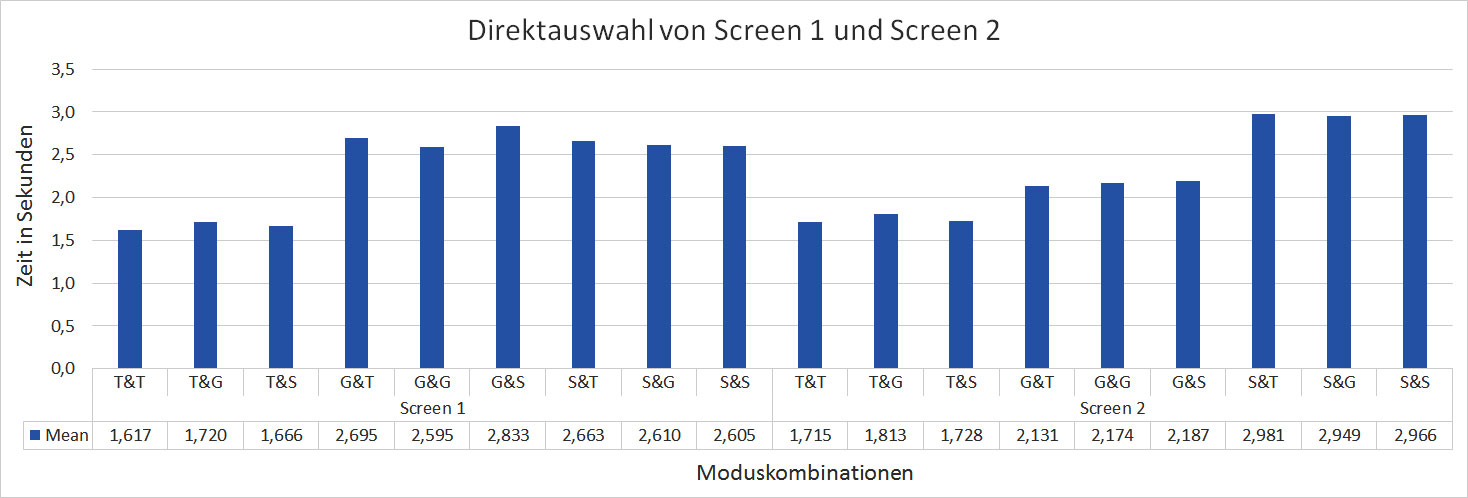
\includegraphics[width=1\textwidth]{img/DA_Screen12.JPG}
  \caption[Durchschnittszeiten in Sekunden der Direktauswahl]{Durchschnittszeiten und Medianwerten in Sekunden der Direktauswahl beider Screens für alle Modalitätskombinationen. T steht für Touch, S für Sprache und G für Geste.}
  \label{fig:DA_Screen12}
\end{figure}

In \fref{fig:DA_Screen12} werden die Durchschnittszeiten von allen Modalitätskombinationen der ersten beiden Screens abgebildet. 
Für die erste Aktion spielt auch nur die erste Modalität eine Rolle, da ein Wechsel der Modalitäten erst anschließend statt findet. 
Die Auswahl der Kachel per Touch ist auf beiden Screens am schnellsten. 
Im ersten Screen liegen die Interaktionszeiten für Geste und Sprache sehr nah zusammen. 
Im zweiten Screen dauert die Spracheingabe deutlich länger als per Gestensteuerung.
Wie zu erwarten scheint die nachfolgende Modalität keinen großen Einfluss auf die Interaktionszeit zu nehmen. 
Uns interessiert im speziellen der Einfluss nach einem Wechsel. 

Als nächstes stellen wir Aktionen vor, die nach einem potentiellen Modalitätswechsel statt finden. 
Die Modalität, die in dieser Aktion ausgeführt wird ist somit die jeweils zweite Modalität. 
Im Falle der unimodalen Variante findet kein Modalitätswechsel statt. 

Findet ein Modalitätswechsel statt, bezeichnen wir im folgenden die zusätzliche Zeit als Vorbereitungskosten. 
Sie beinhalten einen mentalen Operator und den Homing Operator, da bei einem Modalitätswechsel zu Geste oder Touch die Position der Hand geändert wird.

Die erste Aktion, die wir uns nach einem Modalitätswechsel ansehen, ist die Aktion Listen-Navigation (L). 
Die Probanden mussten im Anwendungsbeispiel Telefon die Liste um drei Seiten inkrementieren und schließlich den Kontakt "`Maria Müller"' durch eine Direktauswahl anrufen. 
Der erste Swipe beinhaltet die Vorbereitungskosten, weswegen dieser auch deutlich länger dauert, als die anderen beiden Swipes siehe \fref{fig:Swipe13Phone}. 
Der Startpunkt des ersten Swipes ist der Zeitpunkt, sobald der Screen mit der Liste geladen wurde. 
Wurde die Liste um eine Seite gescrollt, ist dies die Endzeit des ersten Swipes und gleichzeitig die Startzeit des zweiten Swipes.
Das selbe gilt für den dritten Swipe.

\begin{figure}[ht]
  \centering
  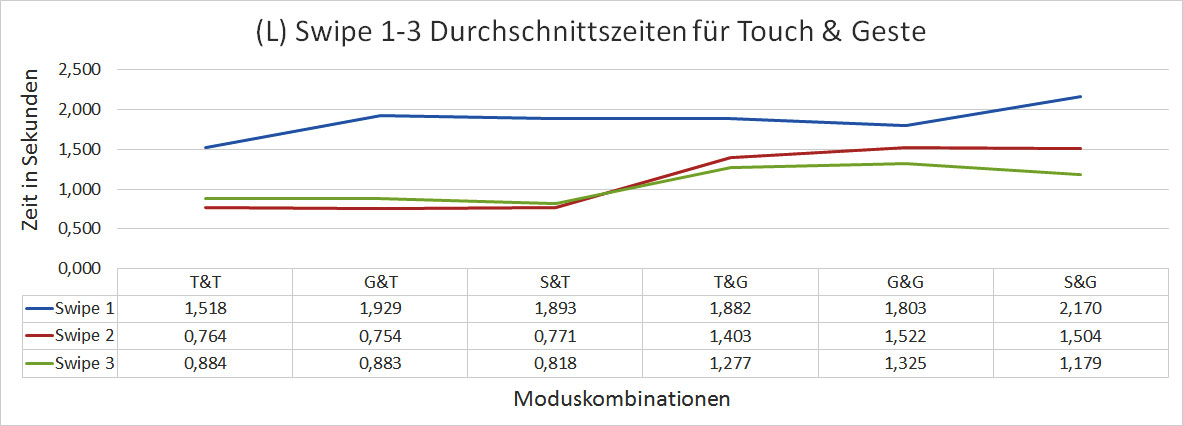
\includegraphics[width=1\textwidth]{img/Swipe1-3_Phone.JPG}
  \caption{Durchschnittszeiten für Swipe 1, 2 und 3 in Sekunden der Liste für die Modalitätskombinationen von Touch und Geste}
  \label{fig:Swipe13Phone}
\end{figure}

Es fällt auf, dass beim ersten Swipe die unimodalen Varianten schneller sind als die multimodalen Varianten. 
Der Wechsel einer Modalität benötigt etwas mehr Zeit, da der mentale Operator wahrscheinlich etwas höher ist.
Des Weiteren fällt die Umpositionierung der Hand weg. 

Anschließend folgt die Aktion Direktauswahl innerhalb der Liste von "`Maria Müller"', siehe \fref{fig:DA_Swipe}. 
Hier ist eine deutlich kürzere Zeit zu beobachten als bei Direktauswahl des ersten Screens, da sich die Hand des Nutzer bereits im richtigen Interaktionsbereich befindet. 
Daher sollten wir diese Aktionen zusätzlich unterscheiden. 
Die Direktauswahl aus sichtbaren Elementen innerhalb der Liste startet unmittelbar nach dem dritten Swipe und endet mit der Selektion der Kachel "`Maria Müller"'.
\begin{figure}[ht]
  \centering
  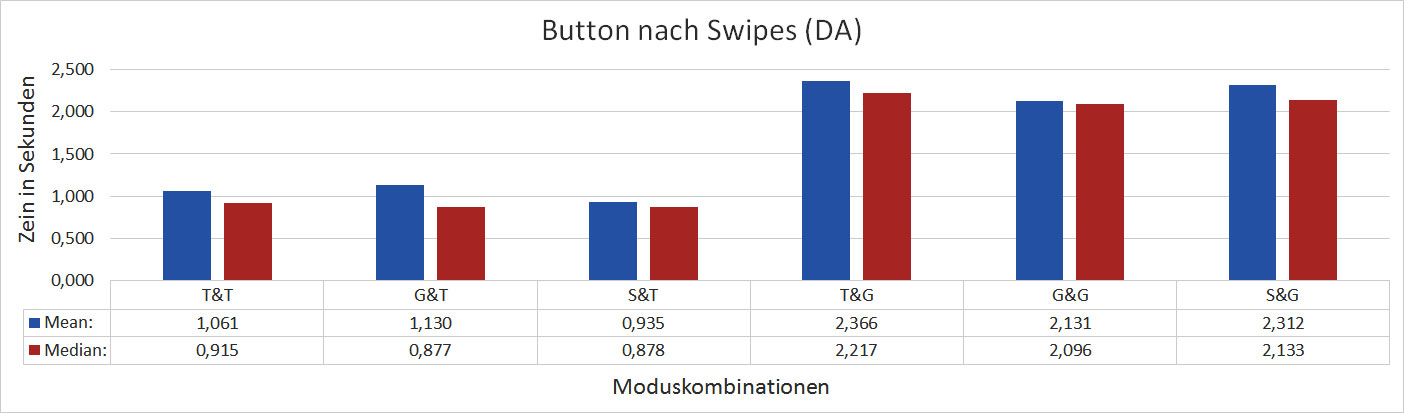
\includegraphics[width=1\textwidth]{img/DA_Swipe.JPG}
  \caption{Durchschnittszeiten in Sekunden für die Direktauswahl innerhalb der Listen Aktion}
  \label{fig:DA_Swipe}
\end{figure}

Die Touchzeiten der Texteingabe durch Buchstaben, der drei verschiedenen Ziele können aus \fref{fig:TouchzeitenB_Ges} entnommen werden.
Der Start der Texteingabe beginnt wieder mit dem Laden der Szene des Texteingabescreens.
Jeder Buttonklick eines Buchstaben ist die Endzeit des vorherigen Buchstaben und die Startzeit des nächsten Buchstabens.
Auch hier ist ein deutliches Muster zu erkennen. 
Der erste Buchstabe dauert am längsten, da hier erneut die Vorbereitungskosten hinzukommen. 
Auch bei dieser Aktion ist die unimodale Variante mit 1,765 Sekunden (Touch-Touch) im Durchschnitt schneller als die Multimodalen Varianten mit 1,990 Sekunden (Geste-Touch) und 1,983 Sekunden (Sprache-Touch).
Der zweite und dritte Buchstabe ist schon deutlich schneller und alle weiteren Buchstaben nähern sich dem Wert einer halben Sekunde an. 
\begin{figure}[ht]
  \centering
  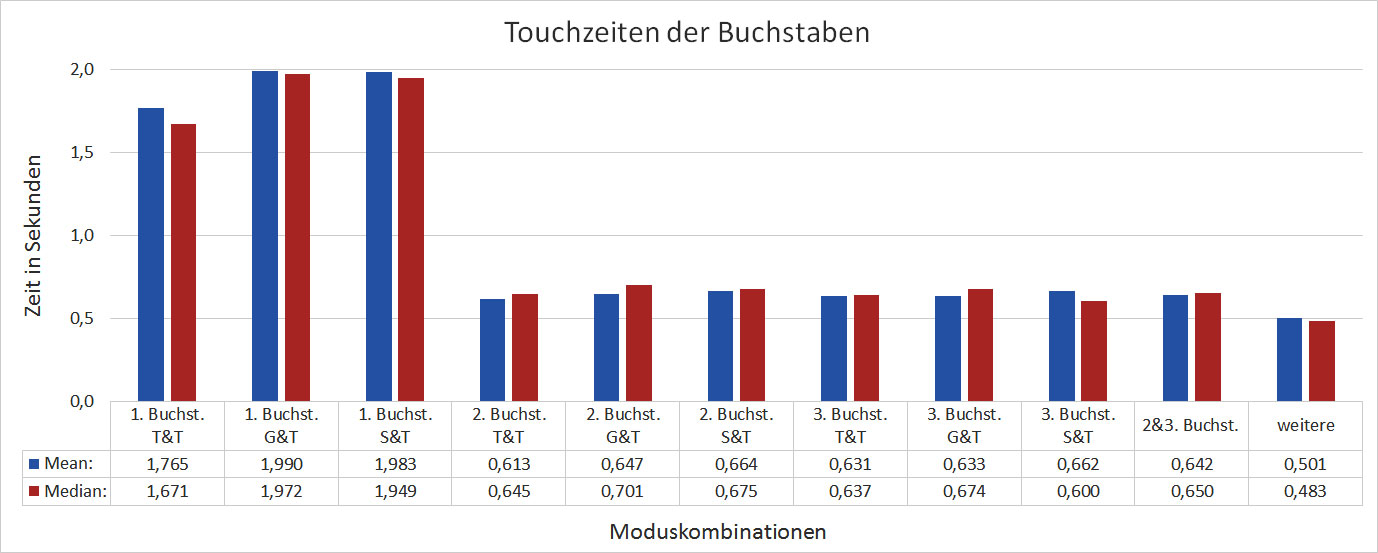
\includegraphics[width=1\textwidth]{img/TouchzeitenBuchstabenGesamt.jpg}
  \caption{Durchschnittszeiten für Touch in Sekunden der einzelenen Buchstaben}
  \label{fig:TouchzeitenB_Ges}
\end{figure}
\begin{figure}[ht]
  \centering
  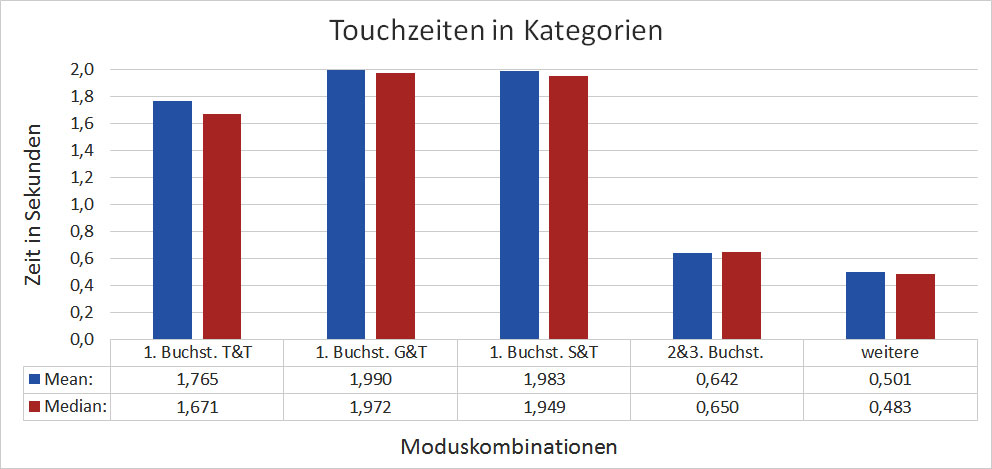
\includegraphics[width=1\textwidth]{img/TouchzeitenKategorien.JPG}
  \caption[Kategorien der Buchstaben für Wörter.]{Kategorien der Buchstaben für Wörter. Hier wurden von den drei verschienenen Zielen ("`Rom"', "`Dorfweg"' und "`Kirchengasse"') jeweils die ersten, zweiten und dritten und alle weiteren Buchstaben zusammengefasst.}
  \label{fig:Kategorien}
\end{figure} 

In \ref{fig:TouchzeitenB_Ges} lässt sich deutlich erkennen, dass sich der zweite und dritte Buchstaben nicht deutlich unterscheiden und die restlichen Buchstaben nochmals schneller eingegeben wurden. 
Wir haben uns deshalb entschlossen beim ersten Buchstaben die vorherige Modalität zu unterscheiden. 
Den zweiten und dritten Buchstaben fassen wir zusammen und für alle weiteren Buchstaben berechnen wir den Durchschnitt dieser. 
Wir haben somit drei Kategorien.
Der erste Buchstabe mit Unterscheidung der vorherigen Modalität, eine gemeinsame Zeit für den zweiten und dritten Buchstaben und als letztes, eine Zeit für alle weiteren Buchstaben \ref{fig:Kategorien}.

Bei der Sprache ist das Ergebnis weniger deutlich (siehe \ref{fig:SpracheZiel}).
Allerdings ist klar zu erkennen, dass "`Rom"' am schnellsten eingegebn werden konnte. 
Zwischen "`Dorfweg"' und "`Kirchengasse"' ist keine eindeutiger Unterschied zu erkennen. 
Auch hier ist das Laden der Szene die Startzeit und die Endzeit ist die Zeit, zu der das Inputfeld mit dem Ziel gefüllt wird.
\begin{figure}[ht]
  \centering
  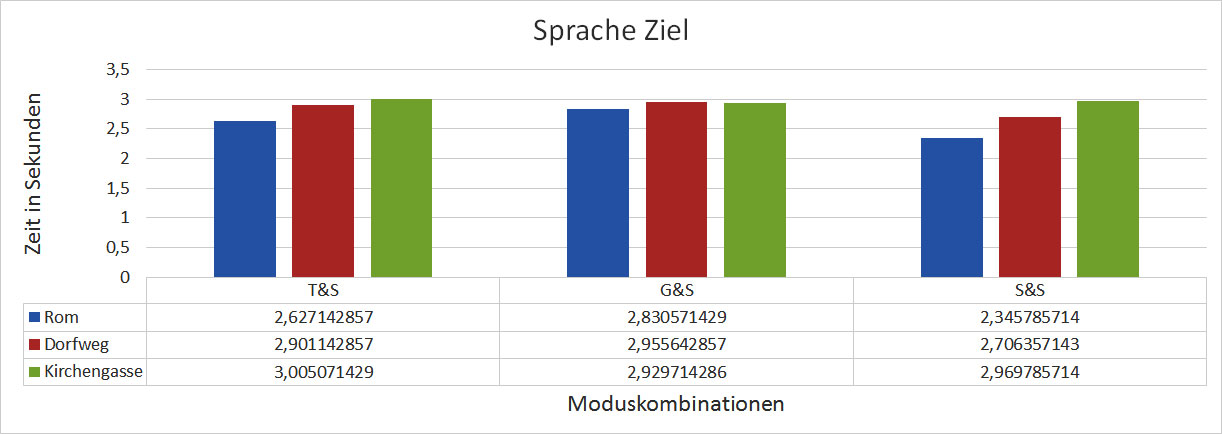
\includegraphics[width=1\textwidth]{img/SpracheZiel.JPG}
  \caption{Durchschnittszeiten in Sekunden der Ziele für Sprache}
  \label{fig:SpracheZiel}
\end{figure} 

Nach dem Touch und den Spracheingaben der Ziele wird noch die Bestätigung des "`Ok"'-Buttons gemessen. 
Die Aktion startet mit dem letzten Buchstaben der Touch-Eingabe oder dem Aktualisieren des Inputfeld durch die Spracheingabe. 
Der Modalitätswechsel fand bereits statt und wie zu erwarten sind die Abweichungen zur vorherigen Modalität sowohl bei Touch, als auch bei der Spracheingabe sehr gering (siehe \ref{fig:Bestaetigung_OK}).
\begin{figure}[ht]
  \centering
  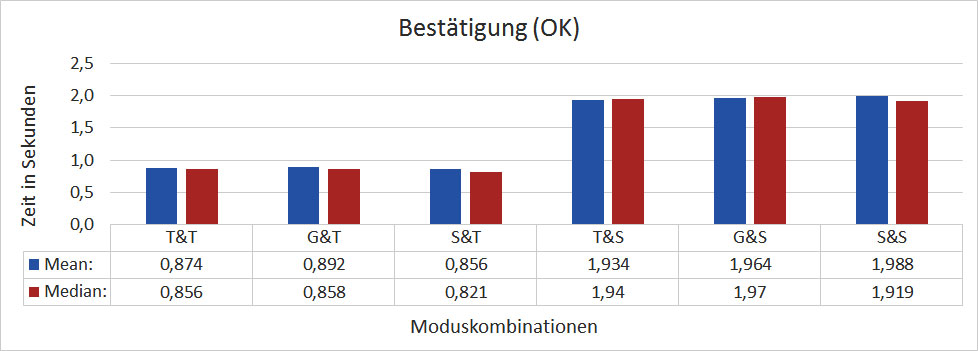
\includegraphics[width=1\textwidth]{img/B_OK.jpg}
  \caption{Durchschnittszeiten und Medianwerte in Sekunden für die Bestätigung der Texteingabe.}
  \label{fig:Bestaetigung_OK}
\end{figure} 

Im Anwendungsbeispiel Medien folgt im dritten Screen die Aktion direkte Inkrementation (Inkr. (d)) durch den Slider (siehe \fref{fig:Slider}) mit einem anschließendem Popup (siehe \fref{fig:Popup}). 
Auch hier ist das Laden der Szene die Startzeit der Aktion. 
Sobald der Slider im gewünschten Bereich von 75-85\% losgelassen wird endet die Aktion und das Popup wird sichtbar. 
Das Ende der Aktion Inkr. (d) ist der Start der Bestätigungsaktion B. 
Diese wiederum endet mit der Selektion des Popups.
\begin{figure}[ht]
  \centering
  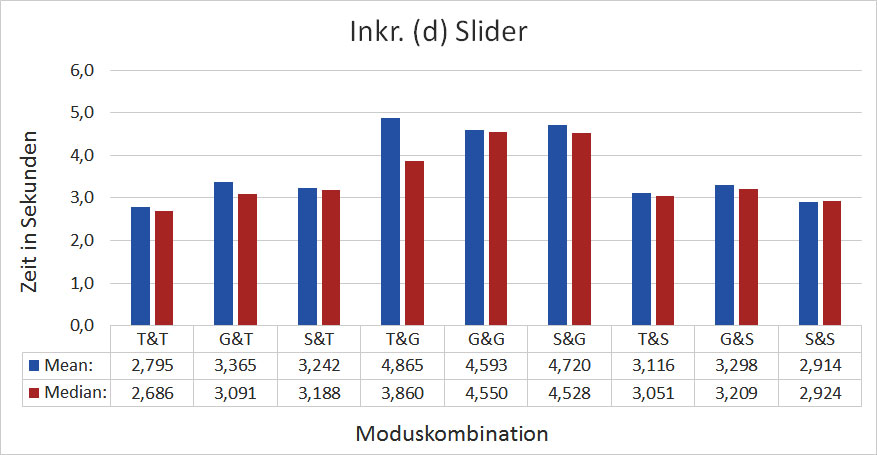
\includegraphics[width=1\textwidth]{img/Slider.JPG}
  \caption[Durchschnittszeiten für Inkr. (d)]{Durchschnittszeiten in Sekunden für die Aktion Inkr. (d) des Sliders, der von 50 auf 75 bis 85 Prozent für alle Kombinationen eingestellt werden soll.}
  \label{fig:Slider}
\end{figure} 
\begin{figure}[ht]
  \centering
  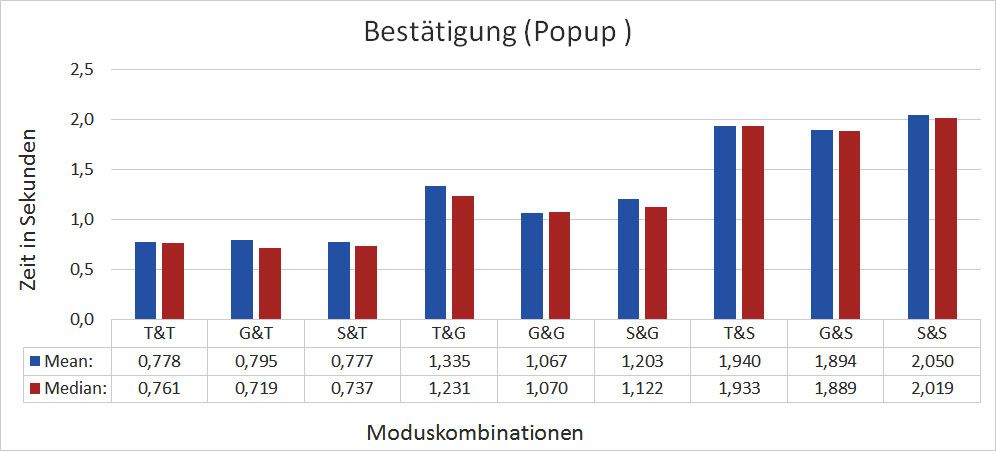
\includegraphics[width=1\textwidth]{img/PopupBestaetigung.JPG}
  \caption[Durchschnittszeiten für die Bestätigung des Popups]{Durchschnittszeiten in Sekunden für die Bestätigung des Popups, für alle Kombinationen der Modalitäten}
  \label{fig:Popup}
\end{figure} 
Auch bei den Zeiten für (Inkr. (d)) bestätigt sich erneut, dass die unimodalen Varianten schneller sind als die multimodalen Varianten. 
Bei dem anschließenden Popup hat der Modalitätswechsel bereits stattgefunden und es ist zu erkennen, dass die Zeiten hier von der vorherigen Modalität nicht abhängen.

Als letzte Aktion bleibt noch die stufenweise Inkrementation Inkr. (s) im Anwendungsbeispiel Temperatur (siehe \fref{fig:SwipeKlima}). 
Die Aktion beginnt mit dem Laden der Szene für die Einstellung der Temperatur. 
Der erste Swipe endet genau wie bei der Listen-Navigation (L) mit dem Erreichen der nächsten Seite. 
Hier startet gleichzeitig der nächste Swipe, bis wir nach dem dritten Swipe bei der gewünschten Seite angekommen sind. 
Es folgt eine Verzögerung bis der Wert eingeloogt wird. 
Diese wird in die Gesamtzeit nicht miteinbezogen, da das Ziel bereits erreicht wurde. 

Auch hier ist deutlich zu sehen, dass der erste Swipe am längsten dauert, Swipe 2 und 3 hingegen sehr ähnlich sind. 
Beim ersten Swipe sind die unimodalen Varianten ebenfalls schneller als die multimodalen Varianten.
\begin{figure}[ht]
  \centering
  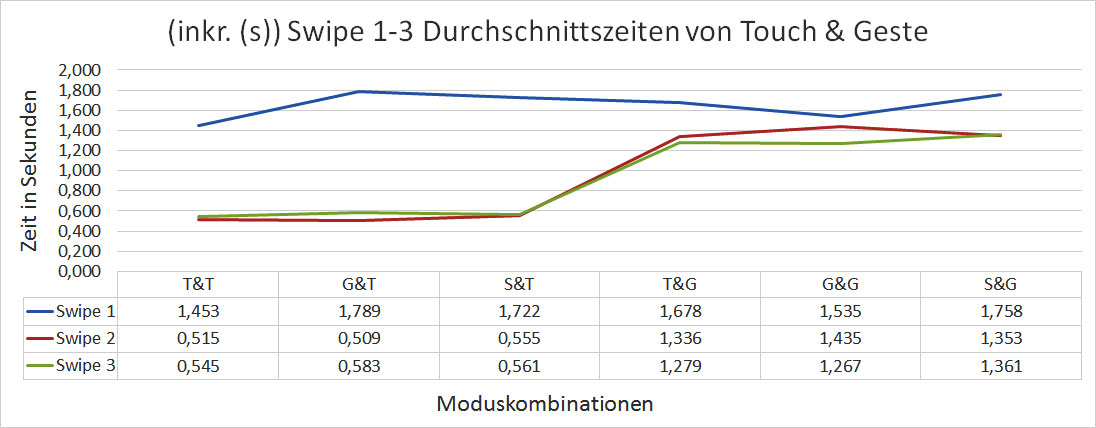
\includegraphics[width=1\textwidth]{img/Swipe1-3_Klima.JPG}
  \caption[Durchschnittszeiten für Inkr. (s)]{Durchschnittszeiten für Swipe 1, 2 und 3 in Sekunden der Wertinkrementation für die Kombinationen der Modalitäten Touch und Geste}
  \label{fig:SwipeKlima}
\end{figure} 

Wir haben jetzt unsere Aktionen ausgewertet und einen Blick auf die verschiedenen Zeiten geworfen.
Im Folgenden werden die Zeiten auf statistisch signifikante Unterschiede untersucht. 

\subsection[Statistische Tests]{Statistische Tests der Aktionszeiten}
Mit einer One-Way Repeated Measures ANOVA wurde mit Hilfe von SPSS für jede Aktion geprüft, ob die zweite Modalität einen signifikanten Einfluss auf die erste hat und vor allem, ob die erste Modalität einen signifikanten Einfluss auf die zweiten Modalität hat. 
Die abhängigen Variablen waren dabei die Modalitäten (Touch, Geste und Sprache) und es wurden die wiederholten Messungen der Zeiten verglichen. 

Bei diesem Test muss beachtet werden, dass die Sphärizität nicht verletzt wird. 
\citet{field2002design} erklärt in seinem Buch "`How to Design and Report Experiments"' wie dies in SPSS berücksichtigt wird. 
Ist bei Mauchly's Test der Sphärizität das Ergebnis signifikant wird die Sphärizität verletzt und es muss eine Korrektur vorgenommen werden. 
Wir verwenden bei unseren Ergebnissen für eine Korrektur, die Greenhouse-Geisser Korrektur. 
Ist bei Mauchly's Test der Sphärizität das Ergbenis nicht signifikant, ist die Sphärizität auch nicht verletzt und es kann beim Test der Inner-Subjekt Effekten der Wert aus der Zeile entnommen werden, indem die Sphärizität angenommen wird \citep{field2002design}.

Diese Auswertung zur Überprüfung von signifikanten Unterschieden wurde für jede Aktion innerhalb ihrer Modalität überprüft. 
Die Ergebnisse werden im Abschnitt \ref{sec:Herleitung} präsentiert.

\section[Herleitung des Modells]{Ableitung des multimodalen Modells aus den gewonnen Interaktionszeiten}\label{sec:Herleitung}
Aus unserer Studie haben wir Zeiten für verschiedene Aktionen in den jeweiligen Moduskombinationen erhoben. 
Die Zeiten in den folgenden Tabellen sind die Durchschnittszeiten für eine Aktion, der in einer bestimmten Moduskombination ausgeführt wurde. 
Wird eine Aktion in der Modalität Touch (T) ausgeführt gibt es 3 mögliche Modalitäten, die nach einem Wechsel kommen können. 
Entweder ebenfalls Touch und somit Touch\&Touch (TT) oder es folgt Geste und ergibt Touch\&Geste (TG) oder Touch\&Sprache (TS), wenn Sprache nach dem Touch folgt. 
Die gleichen Kombinationen gibt es auch wenn Geste oder Sprache der erste Modus ist. 

Aus unseren Anwendungsbeispielen haben sich verschiedene Aktionen ergeben, die wir jetzt analysieren wollen, um daraus unser Modell abzuleiten. 
In der folgenden Liste werden die einzelnen Aktionen der Anwendungsbeispiele erläutert (siehe auch Anwendungsbeispiele in \fref{fig:UseCases}):
\begin{itemize}
	\item \textbf{DA$_1$, DA$_2$:} Direktauswahl aus sichtbaren Elementen des ersten beziehungsweise zweiten Screens. 
	Dieser beinhaltet beim ersten Screen 4 Buttons, die durch Symbole und Titel gekennzeichnet sind und beim zweiten 3 Buttons, die durch Text auf den Buttons gekennzeichnet sind.
	\item \textbf{L$_1$, L$_2$ und L$_3$:} Der erste (zweite oder dritte) Swipe der Liste aus dem Anwendungsbeispiel Telefon. 
	\item \textbf{DA (L):} Direktauswahl aus sichtbaren Elementen, nachdem im Anwendungsbeispiel Telefon bereits drei mal geswiped wurde und nur noch Maria Müller aus vier Elementen ausgewählt werden muss.	

	\item \textbf{Inkr. (s)$_1$, Inkr. (s)$_2$ und Inkr. (s)$_3$:} Der erste (zweite oder dritte) Swipe der Wertinkrementation aus dem Anwendungsbeispiel Temperatur. 
	\item \textbf{Inkr. (d)} Verschiebung des Sliders im Anwendungsbeispiel Medien. Beim Modus Sprache entspricht das dem Sprachbefehl "`achzig Prozent"'.
	\item \textbf{Popup:} Bestätigung des Popup, das nach dem Slider angezeigt wird.
	\item \textbf{1. Bu., 2. Bu., 3. Bu.:} Der Touch des ersten (zweiten oder dritten) Buchstaben im Anwendungsbeispiel Navigation. 
	\item \textbf{Bu. >3:} Alle weiteren Buchstaben im Anwendungsbeispiel Navigation.
		\item \textbf{Maria M.:} Der Sprachbefehl "`Maria Müller"', der den Kontakt aus einer Liste direkt auswählt. Die Animationszeit, der scrollenden Liste wird nicht berücksichtigt (siehe R(Swipe)). 
		\item \textbf{80 \%:} Der Sprachbefehl "`80\%"', um den Lautstärkeslider zu verstellen.
	\item \textbf{Wort S, M, L:} Kurzes Wort (Rom), mittellanges Wort (Dorfweg) und langes Wort (Kirchengasse).
	\item \textbf{OK:} Bestätigung der Zieleingabe im Anwendungsbeispiel Navigation. 
	\item \textbf{R(Screen):} Konstante Zeit, die vom System benötigt wird von einem Screen auf den nächsten zu wechseln. Ein Wechsel dauert 0,016 Sekunden pro Screenwechsel.
	\item \textbf{R(Swipe):} Beim Modus Sprache wird nach dem Sprachbefehl: "`Maria Müller"' die Liste mit einer Animation zur richtigen Seite geswiped bevor der gewünschte Kontakt ausgewählt wird. Die Zeit dieser Animation nennen wir R(Swipe) und dauert mit unserem Prototypen 1,5 Sekunden.
	\item \textbf{R(DA):} Beim Modus Sprache wurde bei der DA nach jedem Sprachbefehl 0,5 Sekunden gewartet um die gelbe Markierung als Feedback zu sehen. Diese 0,5 Sekunden müssen also bei DA$_1$ und DA$_2$ für die Gesamtzeit hinzugefügt werden.
\end{itemize}
Diese Einzelaktionen wollen wir in diesem Kapitel im Hinblick der Modalitätsunterschiede untersuchen und diese so weit es sinnvoll ist aggregieren, um ein übertragbares Modell zu bekommen.

Für die Sprachbefehle modellieren wir die Zeiten von verschiedenen Wortlängen. 

Für uns am interessantesten in diesem Modell ist, ob ein vorheriger Modus Einfluss auf den nachfolgenden Modus hat und ob und wie sich die Interaktionszeiten dadurch unterscheiden. 
Die Zeiten wurden als Durchschnitt der Zeiten der 22 Probanden ermittelt. 
Die Durchschnittszeiten aller Aktionen sind aus der \fref{tab:OperatorzeitenVorWechsel1}, \fref{tab:OperatorzeitenNachWechsel_TouchGeste} und \fref{tab:OperatorzeitenNachWechsel_Sprache} zu entnehmen. 
\begin{table}[ht]
  \centering
	\begin{tabular}{|l|l|l|l|l|l|l|l|l|l|}
		\hline
		& \multicolumn{3}{|c|}{Touch (T)} & \multicolumn{3}{|c|}{Geste (G)}&\multicolumn{3}{|c|}{Sprache (S)}\\
		\hline
		Aktion 					& TT 		& TG 		& TS 		& GT 		& GG 		& GS 		& ST 		& SG 		& SS\\
		\hline
		DA$_1$ 	& 1,617 & 1,720	& 1,666 &	2,695	&	\textbf{2,595}	&	\textbf{2,833}	&	2,663	& 2,610	& 2,605\\
					&  			&  			&				&				&		\small{$(GS)^*$}					&	\small{$(GG)^*$}			 			&		&	& \\
		\hline
		DA$_2$ 	& 1,715 & \textbf{1,813}	& \textbf{1,728}	&	2,131	&	2,174	&	2,187	&	2,981	&	2,949	& 2,966\\
					&  			& \small{$(TS)^{**}$}				&	\small{$(TG)^{**}$}			&				&				&				&		&	& \\
		\hline			
  \end{tabular}
	\caption[Durchschnittszeiten der Aktionen vor dem Moduswechsel]{Durchschnittszeiten in Sekunden der Aktionen vor dem Moduswechsel. Signifikanz wurde gemessen innerhalb einer Modalität vor dem Wechsel (zum Beispiel TT, TG und TS). Fettgedruckte Zeiten sind signifikant. Unter der Zahl steht zu welcher Kombination diese Zeit signifikant ist. Dabei gilt zusätzlich: * $\text{Signifikanz} \leq 0,05$, ** $\text{Signifikanz} \leq 0,01$ und *** $\text{Signifikanz} \leq 0,001$}
\label{tab:OperatorzeitenVorWechsel1}
\end{table}

\begin{table}[ht]
  \centering
	\begin{tabular}{|l|l|l|l|l|l|l|}
		\hline
		& 					\multicolumn{3}{|c|}{Touch (T)} & \multicolumn{3}{|c|}{Geste (G)}\\
		\hline
		Aktion 					& TT 	& GT 	& ST 	& TG 	& GG 	& SG 	\\
		\hline
		L$_1$				& $\textbf{1,518}$ 				& $\textbf{1,929}$				& $\textbf{1,893}$ 				&	1,902	&	$\textbf{1,797}$					&	$\textbf{2,190}$		\\
									& \small{$(GT, ST)^{***}$}	&	\small{$(TT)^{***}$}			& \small{$(TT)^{***}$}			&				&	\small{$(SG)^{**}$}				&	\small{$(GG)^{**}$}	\\
		\hline
		L$_2$			& 0,764 & 0,758	& 0,771 &	1,403	&	1,529	&	1,504 \\
		\hline
		L$_3$				& 0,884 & 0,883	& 0,818 &	1,271	&	1,336	&	1,191	\\
		\hline
		DA (L)				& 1,056 & 1,141	& 0,945 &	2,366	&	2,118	&	2,291	\\
		\hline
		Inkr. (s)$_1$				& $\textbf{1,453}$ 				& $\textbf{1,789}$		& $\textbf{1,726}$ 			&	1,672	&	$\textbf{1,536}$			&	$\textbf{1,745}$\\
									& \small{$(GT,ST)^{***}$} 	& \small{$(TT)^{***}$}	& \small{$(TT)^{***}$} 	&				&	\small{$(SG)^{***}$}		&	\small{$(GG)^{***}$}\\
		\hline
		Inkr. (s)$_2$				& 0,523 & 0,509	& 0,555 &	1,336	&	1,435	&	1,350\\
		\hline
		Inkr. (s)$_3$				& 0,552 & 0,583	& 0,561 &	1,279	&	1,266	&	1,361\\
		\hline
		Inkr. (d) 				& $\textbf{2,795}$ & $\textbf{3,365}$	& $\textbf{3,242}$ &	4,865	&	4,593	&	4,720\\		
									& \small{$(GT,ST)^{**}$} & \small{$(TT){**}$}	& \small{$(TT){**}$}  &	&	&	\\	
		\hline				
		Popup 				& 0,778 & 0,795	& 0,777 &	$\textbf{1,335}$		&	$\textbf{1,067}$ &\\	
									& 			& 			&  			&	\small{$(GG)^{*}$}	&	\small{$(TG)^{*}$} &		\\	
		\hline
		1. Bu.  		& $\textbf{1,765}$ 						& $\textbf{1,990}$		& $\textbf{1,983}$ 	&				& 			&   \\
									& \small{$(GT)^{*},(ST)^{**}$}	& \small{$(TT)^{*}$}		& \small{$(TT)^{**}$}&			& 		& 	\\
		\hline	
		2. Bu.  		& 0,613 & 0,647	& 0,664 &			& 			& 	 \\
		\hline
		3. Bu.  		& 0,631 & 0,633	& 0,662 &				& 			& \\
		\hline		
		Bu. >3 			& \multicolumn{3}{|c|}{0,501}&				& 			& 	 \\
		\hline		
		OK  					& 0,838 & 0,892 &	0,856 & 			& 			&  		\\
		\hline
  \end{tabular}
	\caption[Durchschnittszeiten der Aktionen nach dem Moduswechsel]{Durchschnittszeiten von Touch und Geste in Sekunden der Aktionen nach dem Moduswechsel. Signifikanz wurde gemessen innerhalb einer Modalität nach dem Wechsel (zum Beispiel TT, GT und ST). Fettgedruckte Zeiten sind signifikant. Unter der Zahl steht zu welcher Kombination diese Zeit signifikant ist. Dabei gilt zusätzlich: * Signifikanz $\leq 0,05$, ** Signifikanz $\leq 0,01$ und *** Signifikanz $\leq 0,001$}
	\label{tab:OperatorzeitenNachWechsel_TouchGeste}
\end{table}

\begin{table}[ht]
  \centering
	\begin{tabular}{|l|l|l|l|}
		\hline
		& 					\multicolumn{3}{|c|}{Sprache (S)}\\
		\hline
		Aktion 					& TS 	& GS 	& SS\\
		\hline
		Maria M.	
							&	$\textbf{2,961}$						& $\textbf{3,112}$							& $\textbf{2,802}$\\
							&	\small{$(GS)^{*},(SS)^{**}$}	& \small{$(TS)^{*},(SS)^{***}$}	& \small{$(TS)^{**},(GS)^{***}$}\\
		\hline
		80 \% 				&	$\textbf{3,126}$		& $\textbf{3,298}$ 							& $\textbf{2,914}$\\		
									&	\small{$(SS)^{**}$}	& \small{$(SS)^{***}$} & \small{$(TS)^{**},(GS)^{***}$}\\	
		\hline				
		Popup 				&	1,941	& $\textbf{1,906}$ 		& $\textbf{2,100}$\\	
									& 			& \small{$(SS)^{**}$} 	& \small{$(GS)^{**}$}\\	
		\hline	
		Wort S  			& $\textbf{2,627}$	& $\textbf{2,785}$		& $\textbf{2,346}$ \\
									& \small{$(SS)^{*}$}& \small{$(SS)^{***}$}	& \small{$(TS)^{*},(GS)^{***}$} \\
		\hline
		Wort M 				& 2,829 & $\textbf{2,956}$ 	& $\textbf{2,706}$ \\
									& 			& \small{$(SS)^{*}$} & \small{$(GS)^{*}$} \\
		\hline
		Wort L 				&	3,055	& 2,930	& 2,970\\
		\hline		
		OK  					&	1,933	& 1,964	& 1,988\\
		\hline
  \end{tabular}
	\caption[Erste Vereinfachung der Durchschnittszeiten der Aktionen nach dem Moduswechsel]{Durchschnittszeiten von Sprachbefehlen in Sekunden der Aktionen nach dem Moduswechsel. Signifikanz wurde gemessen innerhalb einer Modalität nach dem Wechsel (zum Beispiel TT, GT und ST). Fettgedruckte Zeiten sind signifikant. Unter der Zahl steht zu welcher Kombination diese Zeit signifikant ist. Dabei gilt zusätzlich: * Signifikanz $\leq 0,05$, ** Signifikanz $\leq 0,01$ und *** Signifikanz $\leq 0,001$}
	\label{tab:OperatorzeitenNachWechsel_Sprache}
\end{table}

Um das Modell zu verallgemeinern, fassen wir einige der Zeiten zusammen. 
Alle Aktionen, die nicht unmittelbar nach einem Moduswechsel stattfinden sollen zusammengefasst werden. 
Diese Aktionen unmittelbar nach einem Moduswechsel sind L$_1$ (der erste Swipe aus den Kontakten), Inkr. (s)$_1$ (der erste Swipe, um die Temperatur zu inkrementieren), Inkr. (d) (Einstellung des Sliders) und 1. Bu. (der erste Touch des ersten Buchstaben). 
All diese Aktionen weisen auch signifikante Unterschiede untereinander auf (siehe \fref{tab:OperatorzeitenNachWechsel_TouchGeste}, \fref{tab:OperatorzeitenNachWechsel_Sprache}). 
Die Signifikanz wurde gemessen innerhalb einer Modalität nach einem potentiellen Wechsel. 
Das heißt, die Interaktionszeiten der Modalität Sprache werden auf signifikante Unterschiede zum vorherigen Modus untersucht (TS, GS und SS).
Fettgedruckte Zeiten sind signifikant. Unter der Interaktionszeit steht, zu welcher Kombination diese Zeit signifikant ist. 
Dabei gilt zusätzlich: * Signifikanz $\leq 0,05$, ** Signifikanz $\leq 0,01$ und *** Signifikanz $\leq 0,001$. 

Als ersten fassen wir die Zeiten der direkten Auswahl (DA) zusammen, die vor einem Moduswechsel stattfinden und somit keinen Einfluss eines Wechsel haben können. 
Die Aktion DA$_1$ weist signifikante Unterschiede der unimodalen Variante Geste (GG) zur multimodalen Variante Geste und Sprache (GS) auf. 
Im zweiten Screen gibt es ebenfalls einen signifikanten Unterschied in der Aktion DA$_2$ für Touch zwischen TS und TG (siehe \fref{tab:OperatorzeitenVorWechsel1}). 
Wir werden die Interaktionszeiten trotzdem für jede Modalität zusammenfassen, da wir den möglichen Einfluss eines bevorstehenden Moduswechsels nicht berücksichtigen wollen.
Jetzt haben wir noch sechs verschiedene Durchschnittszeiten (je Touch, Geste und Sprache für DA$_1$ und DA$_2$).

Die Zeiten von DA$_1$ und DA$_2$ unterscheiden sich, jedoch ist es schwer zu begründen an welchen Variablen dieser Unterschied liegt. 
\begin{figure}
	\centering
		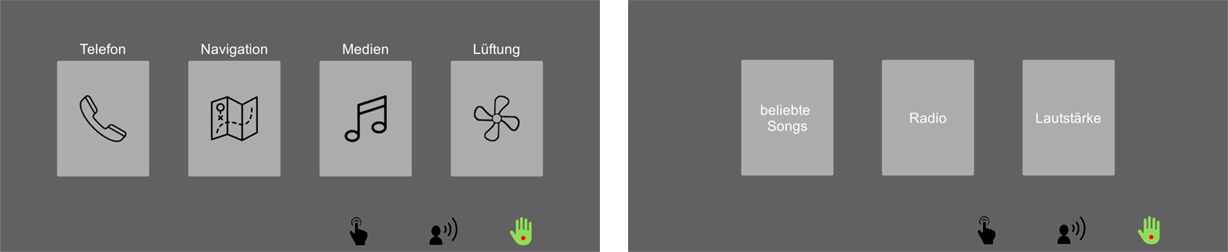
\includegraphics[width=1\textwidth]{img/Screen1vsScreen2.JPG}
	\caption{Unterschiedliche Varianten einer Direktauswahl}
	\label{fig:Screen1vsScreen2}
\end{figure}
Die Größe der Buttons ist zwar gleich, jedoch ist die Anzahl der Buttons unterschiedlich. 
Es gibt auf dem zweiten Screen nur 3 Buttons, statt der 4 Buttons im ersten Screen. 
Außerdem sind im Hauptscreen Icons und Texte dargestellt und auf dem zweiten Screen lediglich Text abgebildet (siehe \fref{fig:Screen1vsScreen2}). 
Wir wollen eine einheitliche Durchschnittszeit der drei Modalitäten für diese Aktion Direktauswahl aus sichtbaren Elementen (DA). 
Also die durchschnittliche Zeit, die für eine Auswahl von 3-4 Buttons der Größe 3,5cm x 4,5cm mit Text oder Icons benötigt wird. 
Deshalb haben wir uns entschlossen die Zeiten zusammenzufassen (siehe \fref{tab:OperatorzeitenZusammengefasst1}).

Als nächstes fassen wir Aktionen zusammen, bei denen der Moduswechsel bereits stattgefunden hat. 
Der erste Swipe beispielsweise ist unmittelbar nach einem potenziellen Moduswechsel. 
Ein Moduswechsel beinhaltet meist einen Homing Operator wie aus dem ursprüngliche KLM. 
Wechselt die Modalität zum Beispiel von Sprache zu Touch, muss die Hand vom Lenkrad genommen werden und sich zum Touchbereich bewegen. 
Nach \citet{Green_2002} würde das dem Operator $R_f$ (Reach Far) Operator entsprechen. 
Eine Aktion unmittelbar nach einem Moduswechsel dauert also länger, was sich aus unseren ermittelten Zeiten auch bestätigen lässt. 

Deshalb fassen wir für den zweiten und dritten Swipe der Liste (L$_2$), (L$_3$) die Modalität vor dem Moduswechsel zusammen. Subtrahieren wir die Durchschnittszeit, die für einen zweiten oder dritten Swipe benötigt wird, von (L$_1$) bekommen wir sozusagen die eine Vorbereitungszeit. Diese Vorbereitungszeit enthält zum Beispiel eine Umpositionierung der Hand und eine mentale Vorbereitung der Aufgabe. Es entsteht also die einheitliche Aktion (L) für alle seitenweise Swipes und zusätzlich eine Vorbereitungszeit, die immer zum ersten Swipe addiert werden muss. Die Vorbereitungszeit unterscheiden wir für jede Modalität und somit entsteht die Aktion V(L), siehe \fref{tab:OperatorzeitenNachWechsel3_TouchGeste}.
 
Das gleiche Vorgehen wenden wir für die Aktion Inkr. (s) an. Auch hier ist der erste Swipe im Schnitt ca. eine Sekunde langsamer als die folgenden. Wir wollen eine einheitliche Aktion Inkr. (s) und zusätzlich eine Vorbereitungszeit V (Inkr. (s)), die für die erste Ausführung benötigt wird. 
 
Bei der Eingabe von Buchstaben per Touch unterscheiden wir die Zeiten zusätzlich in 2 Gruppen. 
Wie wir bereits aus der Abbildung \ref{fig:Kategorien} abgeleitet haben gibt es einerseits auch hier eine deutlich längere Zeit für den ersten Buchstaben. 
Zusätzlich nimmt die Zeit der Touch-Eingabe ab dem vierten Buchstaben nochmal deutlich ab (0,501 statt 0,642 Sekunden). 
Wir modellieren zum einen eine Zeit für das Tippen der ersten 3 Buchstaben und addieren für die Vorbereitung des ersten Buchstabens eine feste Zeit V(1. Bu) hinzu, wie schon bei den Aktionen L und Inkr. (s). 
Für alle weiteren Buchstaben gibt es eine neue geringere Durchschnittszeit, die verwendet werden soll, siehe \fref{tab:OperatorzeitenNachWechsel3_TouchGeste}.  

Im nächsten Schritt werden wir unsere Aktionen für die Modalität Sprache noch vereinfachen, um unterschiedlich lange Wörter unterscheiden zu können. 

Bei der Aktion Swipe Liste muss für die Modalität Sprache lediglich "`Maria Müller"' gesagt werden, um in der Liste zur richtigen Position zu scrollen. Bei der Aktion Inkr. (d) muss "`80 Prozent"' gesagt werden, um den Slider auf 80 Prozent zu verschieben. 
Da beides die Dauer darstellt, die für 2 Wörter benötigt wird, wollen wir diese Zeiten trotz signifikanter Unterschiede zusammenfassen (siehe \fref{tab:OperatorzeitenNachWechsel3_Sprache}). 

Ähnlich dazu, wollen wir die Zeiten für Touch und Sprache des Bestätigungspopups und des Ok Buttons verbinden und diese als einheitliche Aktion Bestätigung (B) zusammen fassen. Sowohl bei Touch, als auch bei Sprache gibt es keine signifikanten Unterschiede zwischen dem Popup und dem Ok Button.

Als letztes fassen wir die Wortlängen M (Dorfweg) und L (Kirchengasse) zusammen. 
Diese sind beide signifikant unterschiedlich zur Wortlänge S (Rom), aber gegenseitig weisen sie keine signifikanten Unterschiede auf. 
Die Unterscheidung der Modalitäten wird allerdings erhalten, da unmittelbar davor der Moduswechsel statt gefunden hat. 
Bei diesen Aktionen wird jetzt lediglich unterschieden, ob sie einsilbig oder mehrsilbig sind. 
Diese Aktionen kürzen wir ab mit Wort(e) für ein einsilbiges Wort und Wort(m) für ein mehrsilbiges Wort (siehe \fref{tab:OperatorzeitenNachWechsel3_Sprache}).

\begin{table}[ht]
  \centering
	\begin{tabular}{|l|l|l|l|l|l|l|l|l|l|}
		\hline
		& \multicolumn{3}{|c|}{Touch} & \multicolumn{3}{|c|}{Geste}&\multicolumn{3}{|c|}{Sprache}\\
		\hline
		Aktion 					& TT 		& TG 		& TS 		& GT 		& GG 		& GS 		& ST 		& SG 		& SS\\
		\hline
		DA 	& \multicolumn{3}{|c|}{1,710} &	\multicolumn{3}{|c|}{2,436} 	&	\multicolumn{3}{|c|}{2,795} \\
		\hline			
  \end{tabular}
	\caption{Zusammengefasste Zeiten der Operatoren vor dem Moduswechsel}
\label{tab:OperatorzeitenZusammengefasst1}
\end{table}
\begin{table}[ht]
  \centering
	\begin{tabular}{|l|l|l|l|l|l|l|}
		\hline
		& \multicolumn{3}{|c|}{Touch (T)} & \multicolumn{3}{|c|}{Geste (G)}\\
		\hline
		Aktion 					& TT 	& GT 	& ST 	& TG 	& GG 	& SG \\
		\hline
		V(L)	& {0,705} 	& {1,116}		& {1,080} 	&	{0,530}		&	{0,425}		&	{0,818}\\
		\hline
		L					& \multicolumn{3}{|c|}{0,813} &	\multicolumn{3}{|c|}{1,372}\\
		\hline
		DA(L)			& \multicolumn{3}{|c|}{1,047} &	\multicolumn{3}{|c|}{2,258}\\
		\hline
		V(Inkr. (s))
										& {0,906} 	& {1,242}		& {1,179} 	&	{0,334}		&	{0,198}		&	{0,407}\\
										& \small{+ 0,547} 	& \small{+ 0,547}	& \tiny{+ 0,547} 	&	\small{+ 1,338}	&	\tiny{+ 1,338}	&	\small{+ 1,338}\\
		\hline
		Inkr. (s)				& \multicolumn{3}{|c|}{0,547} &	\multicolumn{3}{|c|}{1,338}\\
		\hline
		Inkr. (d)				& $\textbf{2,795}$ & $\textbf{3,365}$	& $\textbf{3,242}$ &	4,865	&	4,593	&	4,720	\\		
									& \small{$(GT,ST)^{**}$} & \small{$(TT){**}$}	& \small{$(TT){**}$}  &	&	&		 \\	
		\hline		
		B 				& \multicolumn{3}{|c|}{0,829} &	\multicolumn{3}{|c|}{1,200}\\			
		\hline
		V(1. Bu.)
										& {1,123} 	& {1,348}		& {1,341} 	&				& 			&  	\\
										& \small{+ 0,642} & \small{+ 0,642}	& \small{+ 0,642} &				& 			&  		\\
		\hline	
		1-3. Bu.		& \multicolumn{3}{|c|}{0,642} &				& 			&  	 \\
		\hline		
		Bu. >3 					& \multicolumn{3}{|c|}{0,501} &				& 		&  		\\
		\hline	
  \end{tabular}
	\caption[Zweite Vereinfachung Durchschnittszeiten von Touch und Geste nach dem Moduswechsel]{Durchschnittszeiten von Touch und Geste in Sekunden der Aktionen nach dem Moduswechsel. Signifikanz wurde gemessen innerhalb einer Modalität nach dem Wechsel (zum Beispiel TT, GT und ST). Fettgedruckte Zeiten sind signifikant. Unter der Zahl steht zu welcher Kombination diese Zeit signifikant ist. Dabei gilt zusätzlich: * Signifikanz $\leq 0,05$, ** Signifikanz $\leq 0,01$ und *** Signifikanz $\leq 0,001$}
	\label{tab:OperatorzeitenNachWechsel3_TouchGeste}
\end{table}
\begin{table}[ht]
  \centering
	\begin{tabular}{|l|l|l|l|}
		\hline
		& \multicolumn{3}{|c|}{Sprache (S)}\\
		\hline
		Aktion 					&TS 	& GS 	& SS\\
		\hline
		2 Wörter		&	$\textbf{3,043}$						& $\textbf{3,205}$							& $\textbf{2,858}$\\
								&	\small{$(GS)^{*},(SS)^{**}$}	& \small{$(TS)^{*},(SS)^{***}$}	& \small{$(TS)^{**},(GS)^{***}$}\\
		\hline	
		B						&\multicolumn{3}{|c|}{1,972}\\			
		\hline
		Wort   		& $\textbf{2,627}$	& $\textbf{2,785}$		& $\textbf{2,346}$ \\
		(e)						& \small{$(SS)^{*}$}& \small{$(SS)^{***}$}	& \small{$(TS)^{*},(GS)^{***}$} \\
		\hline
		Wort  			& 2,917 & $\textbf{2,944}$ 	& $\textbf{2,839}$ \\
		(m)						& 			& \small{$(SS)^{*}$} & \small{$(GS)^{*}$} \\
		\hline	
  \end{tabular}
	\caption[Zweite Vereinfachung Durchschnittszeiten von Sprache nach dem Moduswechsel]{Durchschnittszeiten von Sprachbefehlen in Sekunden der Aktionen nach dem Moduswechsel. Signifikanz wurde gemessen innerhalb einer Modalität nach dem Wechsel (zum Beispiel TT, GT und ST). Fettgedruckte Zeiten sind signifikant. Unter der Zahl steht zu welcher Kombination diese Zeit signifikant ist. Dabei gilt zusätzlich: * Signifikanz $\leq 0,05$, ** Signifikanz $\leq 0,01$ und *** Signifikanz $\leq 0,001$}
	\label{tab:OperatorzeitenNachWechsel3_Sprache}
\end{table}

\section[Multimodales Modell]{Multimodales Modell mit Wechselkosten}
In den letzten Schritten haben wir die gesammelten Durchschnittszeiten gruppiert und zusammengefasst. 
Um die verschiedenen Aktionen mit ihren Interaktionszeiten übersichtlich zu einem Modell zusammenzufassen, betrachten wir ab jetzt die Aktionen vorerst unimodal (TT, GG und SS) und addieren je nach Moduswechsel die dementsprechenden Wechselkosten hinzu. 

Die unimodalen Interaktionszeiten waren immer schneller als die multimodalen Interaktionszeiten. Wir verwenden diese als unsere Ausgangszeiten, indem wir sie von den Multimodalen Varianten subtrahieren. Dadurch entstehen dann die sogenannten zusätzlichen Wechselkosten. Zum Beispiel die V(L) dauert für unimodalen Touch (TT) $0,705$ Sekunden und für die multimodale Variante Geste und anschließend Touch (GT) 1,116 Sekunden. Ziehen wir die unimodale Zeit von der multimodalen ab, erhalten wir die Wechselkosten von $0,411$ Sekunden, die bei einem Wechsel von Geste zu Touch (W$_{GT}$) anfallen. 

Wir haben die Aktion (DA) vor einem Moduswechsel für jede Modalität (ergibt 3 Aktionszeiten) und 13 Aktionen nach einem möglichen Moduswechsel für Touch und Geste (ergibt 17 Aktionszeiten) und 4 Aktionen nach einem möglichen Moduswechsel für Sprache identifiziert. 
Dies ergibt 24 Aktionen und 20 verschiedene Arten von Wechselkosten.
Insgesamt kommen wir auf 44 verschiedene Interaktionszeiten für unser Modell.

In \fref{tab:DA} sind die zusammengefassten Zeiten der Aktion DA, die vor dem Moduswechsel stattfinden und in \fref{tab:AktionenUnimodal} sind alle Aktionen mit ihren Interaktionszeiten aufgelistet. Wird eine dieser Aktionen mit einer anderen Modalität ausgeführt als die DA müssen die Wechselkosten addiert werden.
Die dazugehörigen Wechselkosten für multimodale Interaktionen können aus \fref{tab:Wechselkosten} entnommen werden.
\begin{table}[ht]
  \centering
	\begin{tabular}{|l|l|l|l|l|l|l|l|l|l|}
		\hline
		& \multicolumn{3}{|c|}{Touch} & \multicolumn{3}{|c|}{Geste}&\multicolumn{3}{|c|}{Sprache}\\
		\hline
		Aktion 					& TT 		& TG 		& TS 		& GT 		& GG 		& GS 		& ST 		& SG 		& SS\\
		\hline
		DA 	& \multicolumn{3}{|c|}{1,710} &	\multicolumn{3}{|c|}{2,436} 	&	\multicolumn{3}{|c|}{2,795} \\
		\hline			
  \end{tabular}
	\caption{Zusammengefasste Zeiten der Operatoren vor dem Moduswechsel}
\label{tab:DA}
\end{table}
\begin{table}[ht]
  \centering
			\begin{tabular}{|l|l|l|l|}
					\hline
				& \multicolumn{3}{|c|}{Unimodal}\\
				\hline
				Aktion 					& Touch & Geste & Sprache \\
				\hline
				V (L$_1$) 		& {0,705} 	&	{0,425}	&	\\
				\hline
				je (L)				& {0,813} &	{1,372} &\\
				\hline
				DA(L)						& {1,047} &	{2,258} & \\
				\hline
				V(Inkr. (s))		& {0,906} &	{0,198} &\\
				\hline
				Inkr. (s)			& {0,547} &	{1,338} &\\
				\hline
				Inkr. (d)					& {2,795} &	4,593 & \\		
				\hline		
				Bestätigung 		& {0,829} &{1,200} & {1,972}\\			
				\hline
				V(1. Bu.)					& {1,123} 	& 	&\\
				\hline	
				1-3. Bu.					& {0,642} & 	& \\
				\hline		
				Bu. >3 					& {0,501}		&  	& \\
				\hline	
				Wort(e)					& & & {2,346} \\
				\hline		
				Wort(m) 				& & & {2,839}\\
				\hline
				2 Wörter 				& & & {2,858}\\
				\hline
			\end{tabular}
	\caption{unimodale Interaktionszeiten.}
	\label{tab:AktionenUnimodal}
\end{table}
\begin{table}[ht]
  \centering
		\begin{tabular}{|l|l|l|l|l|l|l|}
				\hline
				& \multicolumn{6}{|c|}{Multimodalmodale Wechselkosten}\\
				\hline
				Aktion 					& Geste zu		& Sprache zu 	& Touch zu		& Sprache zu		& Touch zu		& Geste zu\\
												& Touch 			& Touch 			& Geste 			& Geste					& Sprache 		& Sprache \\
				\hline
				L$_1$ 					& ${+0,411}$ 	&	${+0,375}$	& ${+0,105}$ 	&	${+0,393}$		& \multicolumn{2}{|c|}{}	\\
				\hline
				Inkr. (s)$_1$		& ${+0,336}$ 	&	${+0,273}$ 	& ${+0,136}$ 	&	${+0,209}$		& \multicolumn{2}{|c|}{}	\\
				\hline
				Inkr. (d) 					& ${+0,570}$ 	&	${+0,447}$ 	& ${+0,272}$ 	&	${+0,127}$		& \multicolumn{2}{|c|}{}	\\		
				\hline
				1. Buchstabe		& ${+0,225}$ 	& ${+0,218}$ 	&	\multicolumn{2}{|c|}{}			& \multicolumn{2}{|c|}{}	\\
				\hline
				Wort(e) 	& \multicolumn{2}{|c|}{}	& \multicolumn{2}{|c|}{}				& ${+0,281}$ 		& ${+0,439}$\\			
				\hline
				Wort(m)	& \multicolumn{2}{|c|}{}	& \multicolumn{2}{|c|}{}				& ${+0,079}$ 		& ${+0,105}$\\	
				\hline					
				2 Wörter 				& \multicolumn{2}{|c|}{}	& \multicolumn{2}{|c|}{}				& ${+0,185}$ 		& ${+0,347}$\\	
				\hline	
			\end{tabular}
	\caption[Wechselkosten eines Moduswechsels]{Zusatzkosten (Wechselkosten) in Sekunden bei einem Moduswechsel. Diese Wechselkosten betreffen nur Aktionen direkt nach dem Moduswechsel. Wechselkosten müssen bei einem Moduswechsel dementsprechend aufaddiert werden.}
	\label{tab:Wechselkosten}
\end{table}

Zu den Interaktionszeiten ergeben sich noch 3 Antwortzeiten. 
Die Zeit, die für das Laden des nächsten Screens benötigt wird mit einer Antwortdauer von 0,016 Sekunden. 
Um dem Nutzer beim Anwendungsbeispiel Telefon Feedback zu geben, wurde für die Modalität Sprache, nach dem Sprachbefehl "`Maria Müller"' eine Animation eingebaut, die die Liste scrollen lässt, bevor der Kontakt markiert wird. 
Diese Animation dauert 1,5 Sekunden. 
Bei der Spracheingabe zur Direktauswahl aus sichtbaren Elementen wurde eine Verzögerung einer halben Sekunden eingebaut, um die Markierungsfarbe zu sehen. 
Solche konstanten Antwortzeiten (Response Time) sind nicht übertragbar, sondern müssen für jedes zu testende Interface berechnet und in die Vorhersage miteinbezogen werden. Für die Evaluation benötigen wir diese Zeiten.

\section[Qualitative Auswertung]{Qualitative Auswertung der Studie}
Eine qualitative Auswertung kann nicht in Zahlen ausgedrückt werden, sondern beinhaltet Kommentare der Probanden, sowie Beobachtungen des Studienleiters während der Studie.

Eine Studiendauer von 1,5 Stunden pro Proband stellte sich als sehr lange heraus. 
Es konnte beobachtet werden, dass die Konzentration einiger Probanden mit der Zeit nach ließ. 
Hinzu kam, dass es Anfang Dezember sehr kalt in der Parkgarage war. 
Je nach Vorlieben konnte zwar die Sitzheizung eingeschaltet werden, jedoch wurden bei einigen mit der Zeit die Hände kalt. 

Die Verwendung von Gesten als Eingabemodalität erwies sich als sehr unterschiedlich bei den Probanden. 
Obwohl einige Schwierigkeiten bei der Gestenerkennung auftauchten, machte es den meisten sehr viel Spaß damit zu interagieren. 
Es fiel auf, dass Probanden, bei dem die Gesteninteraktion sehr gut funktionierte, auch der Eindruck über Gesteninteraktionen viel positiver war. 
Ein Grund weshalb die Gestenerkennung unterschiedlich gut funktioniert hat, war der festgelegt Interaktionsbereich zwischen Gangschaltung und Dashboard, siehe \fref{fig:GestenbereichSkizze}. 
\begin{figure}
	\centering
		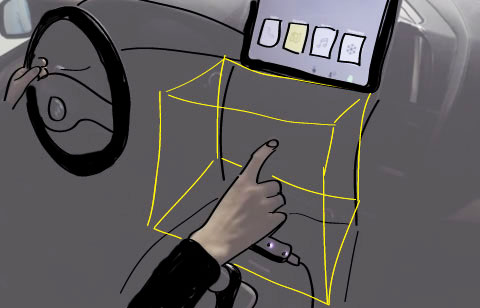
\includegraphics[width=1\textwidth]{img/GestenbereichSkizze2.jpg}
	\caption[Skizze des Interaktionsbereichs zur Gestenerkennung]{Grobe Skizze des Interaktionsbereichs zur Gestenerkennung. Die gelben Markierungslinien bilden den groben Bereich ab, in dem Gesten erkannt wurden.}
	\label{fig:GestenbereichSkizze}
\end{figure}

Die Einstellung des Sitzes und vor allem die Armlänge der Probanden, spielten eine Rolle, ob der Interaktionsbereich bequem erreicht werden konnte. 
Probanden mit längeren Armen war es möglich diesen auf der Armlehne abzulegen und befanden sich trotzdem im Interaktionsbereich. 
Unabhängig von der Armlänge zogen es manche Probanden vor, den Arm während der Gesteninteraktion frei in der Luft zu halten, was auch bei vielen eine gute Gestenerkennung ermöglichte. 
Befindet sich die Hand jedoch zu weit hinten, kommen die Infrarotstrahlen des Leap Motion Controllers nicht durch die Gangschaltung und die Gestenerkennung funktioniert schlechter oder gar nicht. 
Befindet sich der komplette Arm für eine Gesteninteraktion in der Luft, kann dieser bei längerer Dauer schwer werden, was das Ausführen der Gesten erschwert.  

Bei der Touch-Eingabe ist aufgefallen, dass sie zwar keinerlei Schwierigkeiten bei der Interaktion machte, allerdings befand sich der Touchbereich etwas zu weit hinten. 
Einige der Probanden mussten sich etwas nach vorne lehnen, um ihn optimal zu erreichen. 
Das stellt für die Bedienung im stehenden Auto kein Risiko dar, jedoch während der Fahrt sollte das vermieden werden, um möglichst wenig abzulenken. 

Aus Kommentaren einiger Probanden kam heraus, dass sie einerseits die Sprachbedienung für während der Fahrt am geeignetsten halten. Andererseits wurde angemerkt, dass sie die Sprachbedienung eher allein im Auto nutzen würden als mit Mitfahrern. 
Die multimodale Ausführung von Interaktionen kam insgesamt sehr gut an. 
Immer wieder wurde jedoch angemerkt, dass haptische Bedienelemente für die Inkrementation besser geeignet wären. 

\section[Diskussion]{Diskussion zur Studie und Erstellung des Modells}
Bei der Entwicklung des Prototypen und der Erhebung der Interaktionszeiten aus der Studie gab es einige Einschränkungen und Entscheidungen, die im Zusammenhang der Studienergebnisse im folgenden diskutiert und interpretiert werden sollen.

Als erste Einschränkung haben wir die Interaktion mit klassischen haptischen Bedienelementen aus unserer Studie ausgeschlossen. 
Dies lag dem großen Mehraufwand zugrunde, der dabei entstanden wäre. 
Um haptische Bedienelemente befriedigend zu modelliere, müssten, um nur ein Beispiel zu nennen, verschiedene Drehwinkel eines Drehrades gemessen werden \citep{schneegass_2009}. 
Allein durch unsere drei Modalitäten mit Touch, Sprache und Geste entstanden ein Studienumfang von 1,5 Stunden pro Teilnehmer, in der alle Kombinationen der drei Modalitäten getestet wurden. 
Wir haben uns deshalb entschieden, uns in dieser Arbeit auf die Modalitäten Touch, Sprache und Geste zu fokussieren. 

Die Bedienung im Auto durch haptische Knöpfe, Schalter und Regler ist und bleibt ein wichtiger Bestandteil, um Funktionen im Auto zu betätigen. 
Ein großer Vorteil ist, dass die Eingabe oft fast blind getätigt werden kann, ohne die Aufmerksamkeit zu viel von der Straße zu lenken. 
Die Verwendung von haptischen Bedienelementen im Auto wurde bereits in vorherigen Studien untersucht (siehe \citep{Pettitt_2007,schneegass_2009,SchneegaB_2011}. 

In der Studie zur Erhebung von multimodalen Interaktionszeiten verwenden wir keine Fahraufgabe. Stattdessen messen wir die Gesamtdauer (Total Task Time), die in einem stehenden Auto benötigt wird um eine Aufgabe zu lösen. Um den Grad der visuellen Ablenkung, solcher multimodalen Interaktionen messen zu können, sollte unser Modell zusätzlich noch dahingehend erweitert werden, die visuelle Ablenkung miteinzubeziehen (siehe \citep{Pettitt_2007}.
 
Um für alle Kombinationen ausreichend Zeiten erheben zu können musste jeder Nutzer im Within Subject Design alle 33 Kombinationen in durchführen.
Da wir in unserem Modell, wie bei dem Keystroke-Level-Modell \citep{Card_1980}, von Experten ausgehen wollen, mussten die Probanden vorher die Interaktion üben. 
\citet{Jude:2014} zeigte in seinem Paper zu multimodaler Interaktion von Geste und Sprache, dass eine sehr schnelle Interaktionssteigerung mit relativ geringem Training zu beobachten ist. 
Außerdem entschlossen wir uns von jedem Probanden zwei Messdurchgänge zu erheben, um somit die Durchschnittszeit beider Messdurchgänge verwenden zu können. 
Diese Vorkehrungen bedeuteten allerdings, dass die Studiendauer bis zu 1,5 Stunden pro Durchlauf dauerte (je nachdem wie viel geübt werden musste). 

Durch unsere Permutation aller Modalitäten und Anwendungsbeispielen, sollten die eventuellen negativen Effekte auf alle Varianten gleichermaßen verteilt sein.

Die Vorerfahrung von Sprache ergab im Durchschnitt 2,32, bei Touch 3,95 und bei Geste 1,86. Die große Erfahrung mit der Touchbedienung lässt sich auf die weitverbreitete Smartphonenutzung zurückführen. Mit der Gestensteuerung haben die Probanden wie erwartet am wenigsten Erfahrung. Acht der 22 Probanden hatten keine Erfahrungen mit der Gestensteuerung und keiner davon nutzt sie regelmäßig. Diese Erfahrungswerte liegen der wenig verbreiteten Anwendungen mit Gesteninteraktionen zu Grunde.

Für die Sprachmodalität haben wir nicht alle Aktionen abgebildet. 
Statt zum Beispiel in einer Liste aus Kontakten durch einen Sprachbefehl "`nächste Seite"' zu scrollen , erschien es uns geeigneter direkt den Kontakt "`Maria Müller"' auszuwählen. Ebenso beim Einstellen der Temperatur oder der Lautstärke wurde der gewünschte Wert direkt, ohne Inkrementation, gesagt.

In unserem multimodalen Modell unterscheiden wir für die Modalität Sprache nur zwischen einsilbigen und mehrsilbigen Wörtern, sowie einer Durchschnittszeit von zwei Wörtern. 
Die Aktion "`2 Wörter"' wurde aus dem Sprachbefehl "`Maria Müller"' und "`80 Prozent"'
gebildet, obwohl signifikante Unterschiede vorlagen. 
Diese Entscheidung wurde getroffen, um eine übertragbare Aktion für andere Prototypen zu erhalten.
In den meisten gängigen Informationssystemen im Auto, die Sprachbedienung verwenden, können ganze Sätze gesprochen werden (zum Beispiel "`navigiere in die Kirchengasse Nummer 17"'). 
Um die Vorhersage einer Dauer eines Satzes zu modellieren müsste unser Modell noch dahingehend genauer untersucht und erweitert werden. 

Die Zeit der Touch-Eingabe, ab dem vierten Buchstaben nimmt nochmal deutlich ab (0,501 statt 0,642 Sekunden), weshalb wir diese als eigene Aktionszeit definiert haben. 
Zu diesem Zeitpunkt hat sich der Nutzer bereits mit der Tastatur vertraut gemacht und somit  verläuft die weitere Eingabe schneller. 
Das Inputfeld im Screen der Texteingabe befand sich unter der Tastatur. 
Bei einer Touch-Eingabe wurde es durch die Hand verdeckt. 
Es sollte sich besser über der Tastatur befinden. 

Die Aktion Direktauswahl aus sichtbaren Elementen sollte noch erweitert werden, dass sie auch nach einem Wechsel modelliert stattfinden kann. 
In unseren Anwendungsbeispielen kam diese Variante nicht vor und konnte somit nicht modelliert werden.

Der Gesteninteraktionsbereich war nicht für alle Probanden optimal, je nach Armlänge konnten die Gesten der Probanden besser und schlechter ausgeführt werden. 
Probanden, bei denen sich der Interaktionsbereich zu weit weg befand, mussten sich mehr darauf konzentrieren die Geste richtig auszuführen, was die Interaktion verlangsamte und die potenzielle Ablenkung vergrößert. 
In der Studie von \citet{Riener:2013:SIG} wurde der Bereich für Gesten untersucht. 
Sie stellten fest, dass die häufigste Gesteninteraktion sich in dem Dreiecks-Bereich von Lenkrad, Rückspiegel und Gangschaltung befindet. 
Unsere Gestenerkennung befand sich somit innerhalb dieses Bereichs. 
Es wäre ein Vorteil, wenn dieser Interaktionsbereich Bereich individuell einstellbar wäre, um die Gestenerkennung so bequem und robust wie möglich zu gestalten.

Auch der Touchdisplay war für einige Probanden zu weite vorne positioniert. Dieser sollte für den Fahrer ohne große Anstrengung erreichbar sein.
Zur Optimierung der Interaktion mit großen Touchdisplays haben \citet{Rumelin:2013} Touchvarianten verglichen und zum Beispiel ein haptisches Element als Orientierungshilfe in den Screen eingebaut, mit dem die Interaktion eines Kuchenmenüs von diesem Punkt aus fast blind getätigt werden kann. 
Um visuelle Überlagerungen von Karten zu verbessern haben \citet{lee2013saliency} die Suche von Elementen durch die präattentive Wahrnehmung durch das Hervorheben von Elementen verbessert und konnten somit Ablenkung reduzieren. 
Es gibt also nicht nur für die Kombination von Modalitäten, sondern auch für jede einzelne Modalität noch Verbesserungspotenzial. 

Grundsätzlich lässt sich sagen, dass die Sprachbedienung am beliebtesten bei den Probanden war. 
Jedoch wurde oft angemerkt, dass Sie diese Modalität nicht mit Mitfahrern verwenden würden. 
Das ist ein gutes Beispiel dafür, warum es sinnvoll ist bei einem IVIS mehrere Modalitäten anzubieten. 
Nach der reinen Sprachbedienung war die zweitbeliebteste Kombination Touch und Sprache, dicht gefolgt von Geste und Sprache. 
Das zeigt, dass multimodale Interaktionen durchaus bei den Probanden gewünscht sind, was aus den Kommentaren auch bestätigt wurde.

Die Aktionen unseres multimodalen Modells sind nicht so feingranular wie die Operatoren aus dem Keystroke-Level-Modell, sondern befinden sich eine Ebene höher. 
Statt separate Zeiten für die mentale Vorbereitung, der Bewegung vom Lenkrad zum Interaktionsbereich und der Bewegung innerhalb eines Interaktionsbereichs zu modellieren, haben wir diese als durchschnittliche Vorbereitungszeit für 3 verschiedenen Aktionen je nach Modalität zusammengefasst. 
Für der Modellierung des Keystroke-Level-Modell wird genau vorgegeben, wann der Experte welche Bewegung macht und wann er sich mental vorbereitet. 

Diese Herangehensweise war uns für unser Modell zu genau und hätte per Videoanalyse ausgewertet werden müssen. 
Um die Akkudauer der Go Pro-Kamera zu verlängern, haben wir die Auflösung verringert. 
Die Bildqualität reichte aus, um die Varianten nachzuvollziehen, für eine Videoanalyse zur Bestimmung von Operatoren ist sie allerdings ungeeignet. 
Es wurden über 22 Stunden Videomaterial aufgenommen.

Unser multimodales Modell enthält Aktionszeiten, die ein geübter Nutzer im Durchschnitt benötigt, um eine bestimmte Aktion in einer bestimmten Modalität auszuführen. 
Das Modell soll eine grobe Abschätzung der Interaktionszeiten in Abhängigkeit der Modalität mit Berücksichtigung der Wechselkosten berechnen. 
Diese Vorhersage einer multimodalen Interaktionsdauer soll Vergleiche zwischen verschiedenen Moduskombination der Aktionen ermöglichen. 
Es ist jedoch zu erwarten, dass die Vorhersage der Interaktionszeiten eventuell nicht ganz so präzise sind, wie die eines Keystroke-Level Modells.

\chapter[Validierung]{Validierung des multimodalen Modells}\label{cha:Evaluation}
Aus gewonnen Interaktionszeiten aus Studie modellierten wir ein multimodales ein Modell, mit deren Hilfe die Dauer multimodaler Interaktionen vorhergesagt werden sollen.
Außerdem können verschiedene Kombinationen aus Modalitäten auf ihre Gesamtdauer vergleichen werden. 

Im nächsten Schritt soll das erstellte multimodale Modell validiert werden. 
Dazu wollen wir in einer zweiten Studie die Gesamtdauer (Total Task Time) von multimodalen Interaktionen messen, um diese mit den Vorsagen des Modells vergleichen zu können. 

\section[Studie zur Validierung]{Studie zur Validierung des entwickelten Modells}
Wir haben die Studie aufgeteilt in einen Übungsteil und den Anwendungsbeispielen, deren Gesamtdauer wir messen wollen. 
Der Übungsteil, enthält ausgewählte Anwendungsbeispiele aus Kombinationen von Modalitäten, die für den zweiten Teil benötigt werden. 
Mit diesen Übungen sollen sich die Probanden mit dem Modalitäten vertraut machen. 
Im zweiten Teil sollen insgesamt fünf Anwendungsbeispiele getestet werden. Für jedes Anwendungsbeispiel wurde eine Kombination von Modalitäten festgelegt. 

Für die Auswahl der fünf Anwendungsbeispiele haben wir die Kombination von Modalitäten explizit so gewählt, dass sie in ihrer Eignung besonders gut waren siehe \ref{fig:Uebersicht_Eignung} oder deren Kombination uns interessiert hat. Die Texteingabe zum Beispiel schnitt für die Sprache deutlich besser ab, als Touch, weshalb wir diese nur mit der Modalität Sprache verwendeten. Außerdem wollen wir auch Beispiele mit mehr als einem Modalitätswechsel testen. 

Das Modell wird nur stichprobenartig validiert, um die Studie in kürzerem Rahmen zu halten. 
Das heißt, in den Anwendungsbeispielen, die wir in der zweiten Studie testen wollen kommen nicht alle modellierten Aktionen vor. 
  
In den filgenden Unterabschnitten werden die Übungsbeispiele und die Anwendungsbeispiele erläutert.  	
\subsection[Übungsbeispiele]{Übungsbeispiele der Validierungsstudie}
Dafür bauen wir den Prototypen etwas um und testen in einer weiteren Studie mit 10 Teilnehmern. Bevor wir mit den Anwendungsbeispielen für die Evaluation beginnen, soll in der Evaluationsstudie erst geübt werden. Dafür verwenden wir die Variante des Prototypen aus der ersten Studie. Die Anwendungsbeispiele sind dort  kürzer und so können sich die Probanden mit den Interaktionen vertraut machen.
Wir haben folgende Übungsvarianten aus der ersten Studie gewählt (siehe \fref{fig:UseCases}):
\begin{enumerate}
	\item Navigation (Geste, Sprache)
	\item Lautstärke (Geste, Touch)
	\item Lautstärke (Sprache, Geste)
	\item Temperatur (Sprache, Touch)
	\item Telefon (Touch, Sprache)
	\item Telefon (Geste, Touch)
\end{enumerate}
Mit diesen Übungsbeispielen wurde die Direktauswahl aus sichtbaren Elementen (DA) mit Geste, Sprache und Touch geübt. Die Listennavigation (L) mit Sprache und Touch. Die direkte Inkrementation (Inkr. (d)) des Sliders mit Touch und Geste und zuletzt die schrittweise Inkrementation (Inkr.(s)) der Temperatureinstellung mit Touch. Das sind alle Interaktionen, die wir evaluieren wollen.
\subsection[Anwendungsbeispiele]{Anwendungsbeispiele der Validierungsstudie}
Nach diesem Übungsdurchgang werden die fünf Anwendungsbeispiele getestet. 
 
Im ersten Anwendungsbeispiel soll die Lüftung auf Stufe 3 gestellt werden, siehe \fref{fig:UseCasesEvalLuft}. Dafür muss zuerst der Lüftungsbutton mit dem Sprachbefehl "`Lüftung"' selektiert werden. Anschließend wird mit drei Swipe-Touchgesten die Lüftung von null auf drei gestellt. Der Wert wird nach einer kurzen Pause von selbst einprotokolliert, es muss also nicht mit einem Tap bestätigt werden.  
\begin{figure}
	\centering
		\includegraphics[width=1\textwidth]{img/UseCases_Eval_Luft.jpg}
	\caption{Anwendungsbeispiel Lüftung mit den Modalitäten Sprache und Touch}
	\label{fig:UseCasesEvalLuft}
\end{figure}
Mit unserem Modell wird die Interaktionsdauer folgendermaßen berechnet:
\[
\textbf{Lüftung} = \text{DA}_\text{S} + R(DA) + V(\text{Inkr.} (s))_\text{T} + 3*\text{Inkr.} (s)_\text{T}  + W_\text{ST} + R(\text{Screen}) =
\]
\[
= 2,795\text{s} + 0,5\text{s} + 0,906\text{s} + 3*0,547\text{s} +  0,273\text{s} + 0,016\text{s} = 6,133\text{s}
\]

Das nächste Anwendungsbeispiel kennen wir auch schon aus der ersten Studie. Es soll die Lautstärke von 50\% auf 80\% erhöht werden, mit den Modalitäten Sprache und Geste, siehe \fref{fig:UseCasesEvalMedienS}. Zuerst wird mit den Sprachbefehlen "`Medien"' und "`Lautstärke"' zweimal die Aktion DA ausgeführt. Anschließend wird mit der Slidegeste die Lautstärke verstellt. 
\begin{figure}
	\centering
		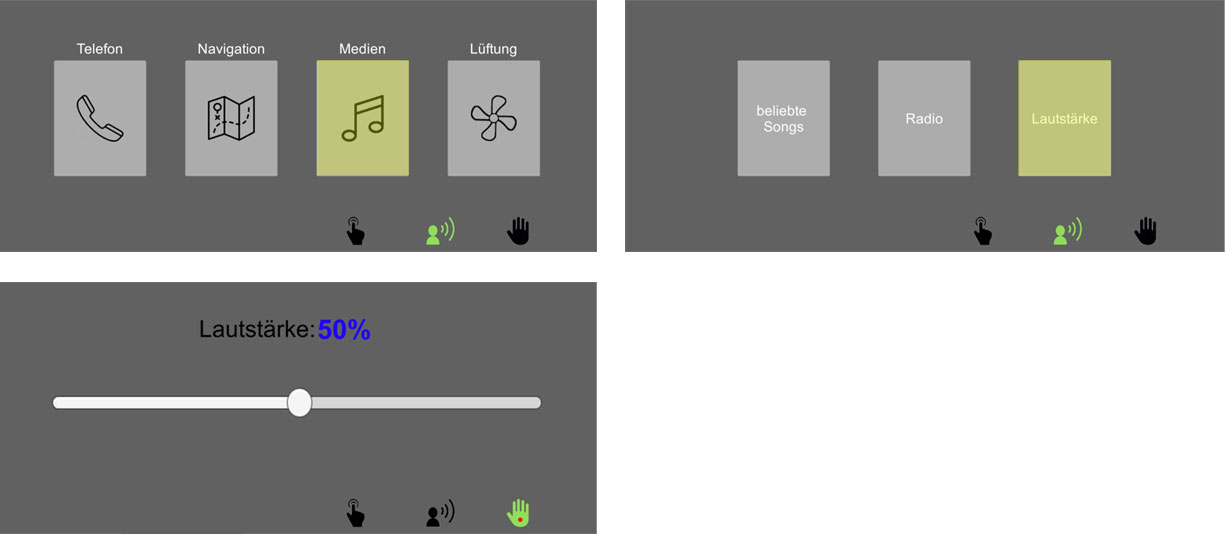
\includegraphics[width=1\textwidth]{img/UseCases_Eval_MedienS.jpg}
	\caption{Anwendungsbeispiel Lautstärke mit den Modalitäten Sprache und Touch}
	\label{fig:UseCasesEvalMedienS}
\end{figure}
Die Berechnung zur Vorhersage der Interaktionsdauer mit unserem Modell sieht wie folgt aus:
\[
\textbf{Medien Sound} = 2*(\text{DA}_\text{S} + R(DA)) + \text{Inkr.} (d)_\text{G} + W_\text{SG} + 3*R(\text{Screen}) =
\]
\[
= 2*( 2,795\text{s} + 0,5\text{s}) + 4,593\text{s} + 0,127\text{s} + 3*0,016\text{s} = 11,358 \text{s}
\]

Im Anwendungsbeispiel Medien, soll zunächst per Geste die DA der Button (Medien) und (beliebte Songs) ausgewählt werden. Es erscheint eine Liste mit beliebten Songs. Mit dem Sprachbefehl "`Happy"' wird das Lied Happy abgespielt. Auf dem nächsten Screen soll mit Touch die Lautstärke geändert werden. Dafür wird per Touch der Lautstärke Button aktiviert. Es erscheint ein Slider, der von 20\% auf 80\% ebenfalls per Touch geändert werden soll. Wird der Slider im Bereich von 75 und 85\% losgelassen kommt ein Popup, dass noch per Touch bestätigt werden muss, siehe \fref{fig:UseCasesEvalMedien}.
\begin{figure}
	\centering
		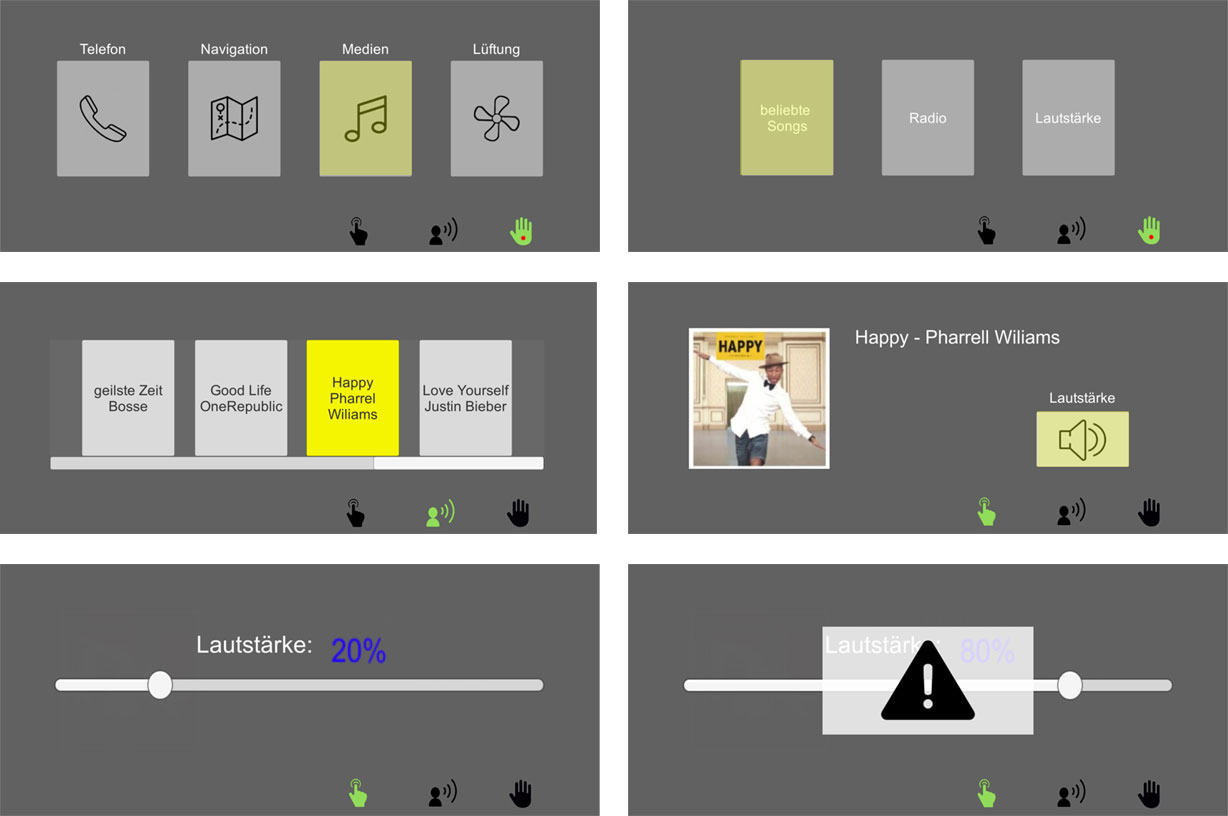
\includegraphics[width=1\textwidth]{img/UseCases_Eval_Medien.jpg}
	\caption{Anwendungsbeispiel Lautstärke mit den Modalitäten Geste, Sprache und Touch}
	\label{fig:UseCasesEvalMedien}
\end{figure}
Die Interaktionszeit besteht aus diesen Aktionen und Wechselkosten:
\[
\textbf{Medien} = 2*(\text{DA}_\text{G}) + \text{Wort(m)}_\text{S} + W_\text{GS} + V(\text{1. Bu.})_T + \text{1-3 Bu.} + W_\text{ST} + 
\]
\[
 + Inkr.(d)_\text{T} + B_\text{T} + 6*R(\text{Screen}) =
\]
\[
= 2*( 2,436\text{s}) + 2,839\text{s} + 0,105\text{s} + 1,123\text{s} + 1,495\text{s} + 0,218\text{s} +
\]
\[
+2,795\text{s}+0,829\text{s} + 6*(0,016) = 15,014\text{s}
\]

Im nächsten Anwendungsbeispiel wollen wir mit den Modalitäten Geste, Sprache und Touch den nächsten Coffeeshop finden. Dazu werden per Geste die Buttons "`Navigation"' und "`Points of Interest"' ausgewählt. Dann kommt ein Texteingabefeld mit einem Inputfeld zur eingabe des POI. Mit dem Sprachbefehl "`Fastfood"' wird Fastffod im Inputfeld eingetragen. Erneut mit Spracheingabe wird die Eingabe mit "`OK"' bestätigt. Jetzt kommt eine Liste von Fastfood Geschäften. Es muss zum Starbucks auf der zweiten Seite mit Touch geswiped werden. Auf der richtigen Seite angekommen muss noch der Starbucksbutton ausgewählt werden, siehe \fref{fig:UseCasesEvalNaviPOI}.  
\begin{figure}
	\centering
		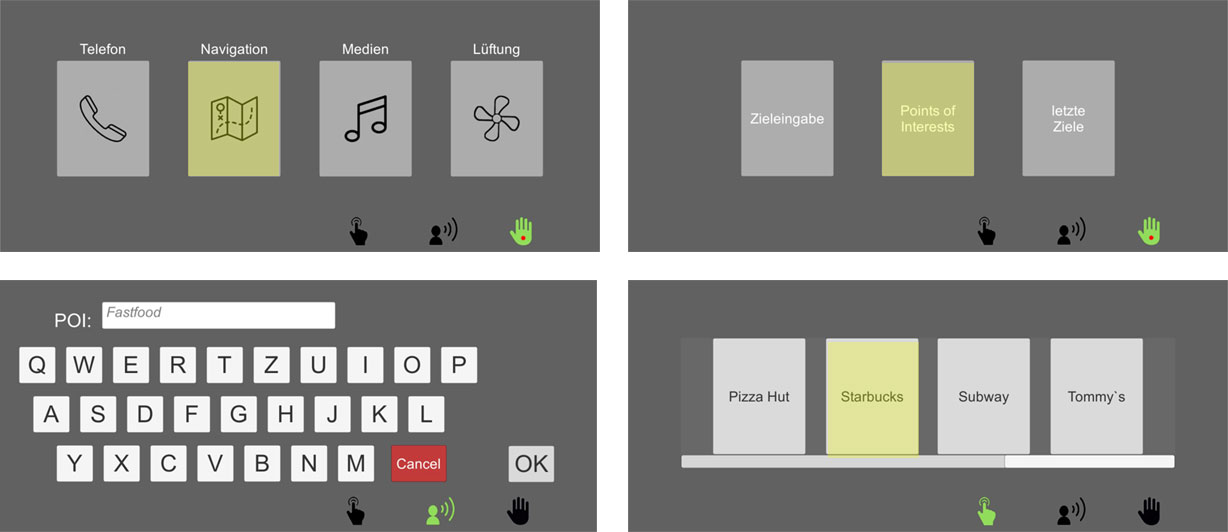
\includegraphics[width=1\textwidth]{img/UseCases_Eval_Navi_POI.jpg}
	\caption{Anwendungsbeispiel Navihation POI mit den Modalitäten Geste, Sprache und Touch}
	\label{fig:UseCasesEvalNaviPOI}
\end{figure}

In der ersten Studie haben wir festgestellt, dass die Positionierung des Inputfeldes oben besser geeignet ist. Auch wenn in unseren Beispielen kein Touch verwendet wird, haben wir diese Anpassung bei den beiden Screens der Texteingabe vorgenommen.

Die Aktionen des Anwendungsbeispiels werden folgendermaßen zusammengesetzt und berechnet:
\[	
\textbf{Navi POI} = 2*(\text{DA}_\text{G}) + \text{Wort(m)}_\text{S} + W_\text{GS} + B_\text{S} + 
\]
\[	
+ V(\text{L})_T + 2*(L)_T + W_\text{ST}(L_T) + DA(L)_T + 4*R(\text{Screen}) =
\]
\[
= 2*( 2,436\text{s}) + 2,839\text{s} + 0,105\text{s} + 1,972\text{s} + 
\]
\[
= + 0,705\text{s} + 2*0,813\text{s} + 1,495\text{s} + 0,375\text{s} + 1,047\text{s} + 4*0,016= 13,605\text{s}
\]

Das letzte Anwendungsbeispiel heißt Navigation Nummer. Hier werden 2 Modalitäten (Touch und Sprache) mit vier Moduswechseln verwendet. Per Touch werden die Buttons Navigation und Zieleingabe gedrückt. Dann kommt ein Texteingabefeld mit zwei Inputfeldern (Straße und Nummer). Um ein Inputfeld zu aktivieren soll der Proband auf das Inputfeld Straße tapen. Dann soll die Straße "`Parkring"' per Sprache eingegeben werden. Anschließend wird erneut mit einem Tap auf das Nummer-Inputfeld	dieses aktiviert. Wieder mit Sprache wird die Nummer "`19"' eingegeben. Als letztes wird mit einem Tap auf den OK-Button die Eingabe bestätigt, siehe (\fref{fig:UseCasesEvalNaviNummer}).
\begin{figure}
	\centering
		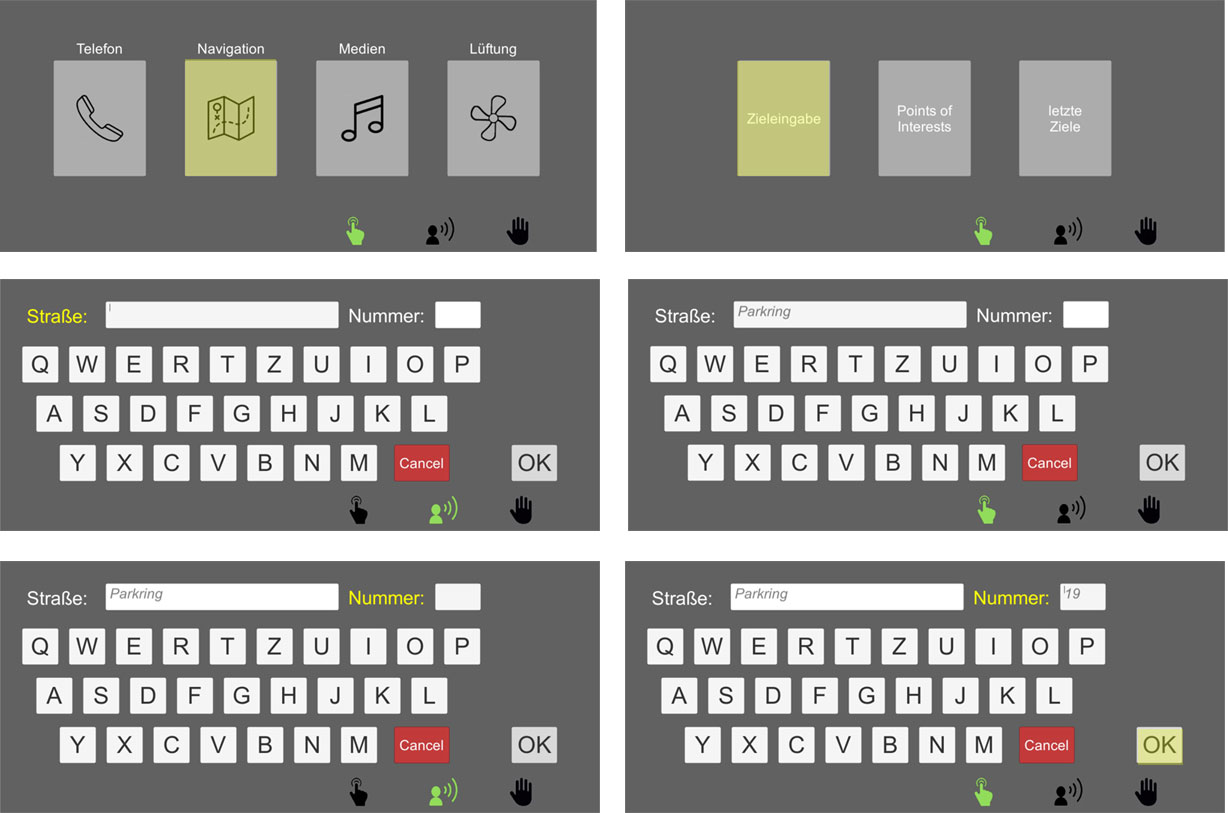
\includegraphics[width=1\textwidth]{img/UseCases_Eval_Navi_Nummer.jpg}
	\caption{Anwendungsbeispiel Navihation POI mit den Modalitäten Touch, Sprache, Touch, Sprache, Touch}
	\label{fig:UseCasesEvalNaviNummer}
\end{figure}	
Auch hier berechnen wir mit unserem erstellten Modell die potenzielle Interaktionsdauer. Sie setzt sich aus diesen Aktionen zusammen:
\[
\textbf{Navi Nummer} = 2*(\text{DA}_\text{T}) + V(\text{1. Bu.})_T + \text{1-3 Bu.}_T + \text{Wort(m)}_S + W_\text{TS}(Wort(m)) +
\]
\[
+ V(\text{1. Bu.})_T + \text{1-3 Bu.}_T + W_\text{ST}(1. Bu.) + \text{Wort(m)}_\text{S} + W_\text{TS} + B_\text{T} + W_\text{ST} + 4*R(\text{Screen}) =
\]
\[
= 2*( 1,710\text{s}) +  1,123\text{s} + 0,642\text{s} + 2,839\text{s} + 0,079\text{s} + 1,123\text{s} + 
\]
\[
+ 0,642\text{s} + 0,218\text{s} + 2,839\text{s} + 0,079\text{s} + 0,642\text{s} + 1,123\text{s} + 0,218\text{s} + 3*0,016 = 15,035\text{s}
\]


\subsection[Studiendesign]{Studiendesign}
Wie in der ersten Studie zur Erhebung von Interaktionszeiten, verwenden wir in der Validierungsstudie ebenfalls ein Within Subject Design, indem jeder Proband alle fünf Anwendungsbeispiele durchführen wird. 
Von jedem der Anwendungsbeispiele werden erneut zwei Messdurchgänge vorgenommen. 
Nach jedem Messdurchgang wurde die Eignung des Anwendungsbeispiel abgefragt und ob das Anwendungsbeispiel dem Probanden gefallen hat.

Die 5 Anwendungsbeispiele wurden mit dem Latin Square permutiert, um auch in dieser Studie mögliche Lerneffekte zu eliminieren. Die Übungsbeispiele zu Beginn eines Studiendurchlaufs wurden jedoch in gleicher Reihenfolge durchlaufen. 

Diese Vorhersage der Interaktionsdauer für unsere 5 Anwendungsbeispiele wird die Grundlage unserer Validierung sein. Wir werden die Anwendungsbeispiel beobachten und mit unseren Vorhersagen vergleichen. 

\subsection[Durchführung der Studie]{Durchführung der Studie}
Die Studie fand unter gleichen Bedingungen wieder bei BMW in Garching-Hochbrück am Parkring 19 in der Parkgarage im gleichen Auto statt. Die Studie dauerte ca. 45 Minuten und wurde in einem Zeitraum von zwei Tagen durchgeführt. Die Einstellungen, der Aufbau sowie die Protokollierung wurde genau wie in der ersten Studie vorgenommen. 

Die Einverständniserklärung, sowie den demographischen Fragebogen verwendeten wir gleichermaßen wie in der ersten Studie. Um dieses mal zusätzlich die Beanspruchung der Interaktionen zu messen wurde nach dem zweiten Messdurchgang jedes Anwendungsbeispiels der NASA TLX abgefragt \ref{cha:Anhang}. Nach den 5 Anwendungsbeispielen wurde der zweite Teil des NASA TLX abgefragt. Hier werden alle 6 Beanspruchungsvarianten gegeneinander verglichen. Die 15 Vergleiche wurden für jeden Probanden geshuffelt, um keinen Einfluss der Reihenfolge zu haben. Außerdem wurde der INTUI Fragebogen abgefragt, um die Usability des Prototypen einzuschätzen. sowie und noch 3 weitere Fragen siehe \ref{cha:Anhang}. 

Wie schon erwähnt konnten sich die Probanden mit den Übungsbeispielen mit den Interaktionen vertraut machen. Sobald die Übungsrunde fertig war wurde die Kamera angeschaltet, um die Evaluationsbeispiele aufzunehmen, für den Fall, dass etwas nachgeprüft werden muss. Bei den Anwendungsbeispielen wurde zusätzlich wie auch bei der ersten Studie jede Aufgabe mindestens einmal geübt. 

Sobald der Versuchsleiter das Gefühl hatte, dass die Aufgabe dem Probanden klar ist wurde mit dem ersten Messdurchgang begonnen. Anschließend der zweite. Traten während eines Messdurchgangs Fehler auf wurde das vom Versuchsleiter notiert ,um den Protokolleintrag im Nachhinein als fehlgeschlagen zu markieren. Dieser Messdurchgang wurde dann wiederholt. Als fehlerhaft wurde ein Messdurchgang gewertet wenn zum Beispiel die Gesten- oder Spracherkennung nicht richtig funktionierte oder wenn der Proband vergaß was er tun muss. 

\section[Auswertung der Studienergebnissen]{Auswertung der Studienergebnissen}
Im folgenden werden nun die Ergebnisse der Evaluationsstudie präsentiert und diskutiert. 
\subsection[Teilnehmer]{Teilnehmer}
In der Evaluationsstudie nahmen insgesamt 10 Teilnehmer (8 männlich und 2 weiblich) teil. Das Alter erstreckte sich von 19-33 Jahren und betrug im Durchschnitt 23,8 mit einen Median von 22 Jahren, also etwas jünger als in unserer ersten Studie (Durchschnitt: 30,55 und Median: 25 Jahre). Alle 10 Teilnehmer sind Rechtshänder und sprechen deutsch als Muttersprache.

Auch in der Evaluation wurde die Vorerfahrungen mit der Bedienung von Touch, Gesten und Sprache der Teilnehmer abgefragt und von den Probanden eingeschätzt. Auf die Frage, ob sie Erfahrung mit der Bedienung von Sprache, Touch und Geste haben, konnte aus vier Optionen gewählt werden (1: nein, 2: ja, aber nur sehr wenig, 3: ja, benutze ich gelegentlich und 4: ja, benutze ich regelmäßig). Die Vorerfahrung der Bedienung von Sprache ergab im Durchschnitt 3,1, bei Touch 4 und bei Geste 2,2. Die Werte sind etwas besser als in unserer ersten Studie (Sprache: 2,32,  Touch: 3,95 und Geste: 1,86), was unter anderem daran liegen könnte, dass die Teilnehmer etwas jünger waren.

\subsection[User Experience]{User Experience}
Im Vergleich zu Touch und Sprache war für die Teilnehmer die Gestensteuerung am ungewohntesten. Die Einschätzung der Eignung der Anwendungsbeispiele mit Geste schnitt nicht so gut ab wie die Anwendungsbeispiele ohne Geste. Allerdings bekam im Anwendungsbeispiel Medien Sound, indem der Lautstärkeslider mit einer Geste verstellt werden sollte, sehr positives Feedback siehe \fref{fig:Smiley_Eignung_Gefallen}. Es wurde auf die Frage, ob Ihnen die Interaktion gefallen würde nur eine negative Antwort gegeben. Nach jedem Messdurchgang (also 2 pro Anwendungsbeispiel) sollten die Probanden auf einer Likertskala mit 5 Unterscheidungen angeben wie geeignet sie die Anwendung fanden und ob es Ihnen gefallen hat.
\begin{figure}
	\centering
		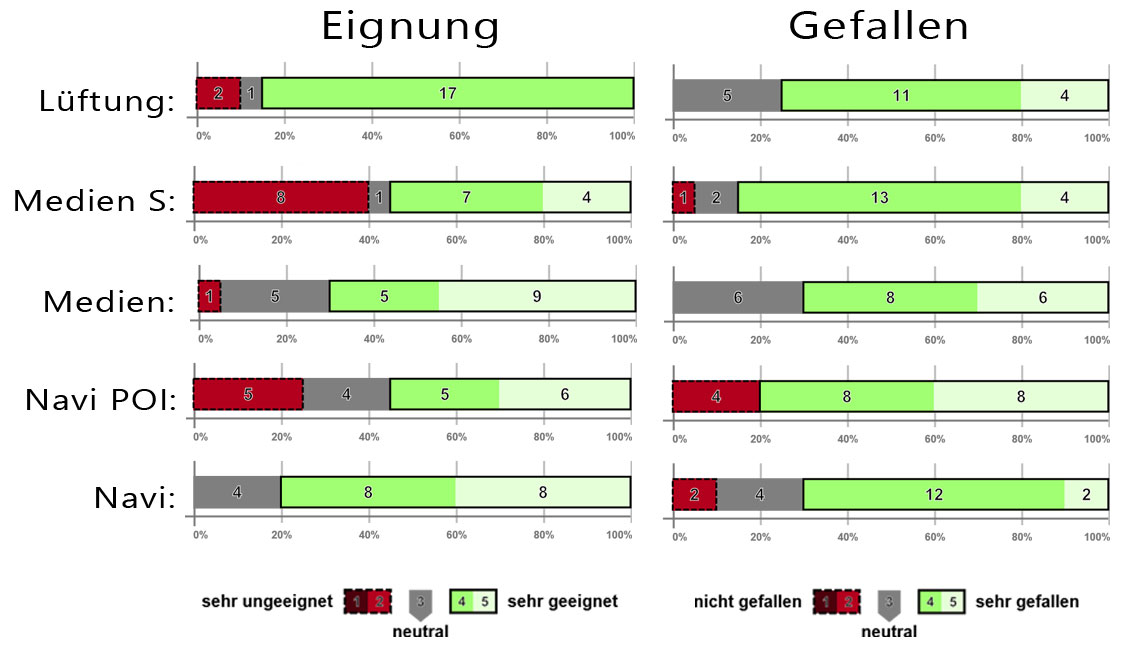
\includegraphics[width=1\textwidth]{img/Smiley_Eignung_Gefallen.jpg}
	\caption[Eignung und Gefallen der 5 Aufgaben]{Eignung und Gefallen der 20 Messdurchgänge der 5 Aufgaben. Die Balkendiagramme zur Darstellung von Likert-Skalen wurde mit http://likertplot.com/ generiert.}
	\label{fig:Smiley_Eignung_Gefallen}
\end{figure}
 
9 von 10 Teilnehmern können sich eine multimodale Interaktion während dem Fahren vorstellen. Begründungen waren die intuitive Bedienung, sowie vor allem der Vorteil sich je nach Situation die passende Modalität frei wählen zu können.

Beim NASA Task Load Index mussten 6 Beanspruchungskriterien auf einer Skala von 1-20 subjektiv von den Probanden bewertet werden. Diese Werte werden alle mit 5 multipliziert, um eine Abstufung von 1-100 zu erhalten. 

Im nächsten Teil wurden alle Kriterien miteinander verglichen und mit diese 15 Vergleichen werden jetzt die Kriterien gewichtet. Wurde die Frustration 4 mal vorgezogen erhält die Frustration eine Gewichtung (G) von 4. Die Bewertung wird also mit 5 und dann mit deren Gewichtung multipliziert. All diese Werte aufsummiert durch 15 geteilt ergeben den gesamten NASA TLX. Diese Gewichtung führt dazu, dass für den Nutzer unwichtige Kriterien weniger bis gar nicht miteinbezogen werden und dafür wichtige um so mehr. 

Sei $B$ die Menge der Beanspruchungen, im speziellen Geistige Anforderung, Körperliche Anforderung, Zeitliche Anforderung, Leistung, Anstrengung und Frustration, dann sieht die Berechnung wie folgt aus:
\[
\textbf{NASA TLX} =\frac{1}{15}\sum_{i \in B}A_{i}G_{i}
\]
wobei $A_i$ der Wert der Beanspruchung ist und $G_i$ die Gewichtung.

Der durchschnittliche NASA TLX jedes Anwendungsbeispiels ist aus der \fref{tab:PredictedVsObserved} zu entnehmen. Das Anwendungsbeispiel Lüftung verursachte mit einem Wert von 25,6 die geringste Beanspruchung. Am meisten beanspruchte das Anwendungsbeispiel Navi Nummer mit den 4 Moduswechseln mit einem Wert von 37,533.
Wir stellen fest, dass mit Dauer der vorhergesagten Interaktionzeiten auch die durchschnittliche Beanspruchung zunimmt.

Im INTUI Fragebogen (siehe Anhang im Kapitel \ref{cha:Anhang}) werden verschiedene Komponenten der intuitiven Nutzung auf einer Skala von 1-7 abgefragt \citep{diefenbach2010handbuch}, \citep{ullrich2010intui}. Die Probanden wurden hierfür darauf hingewiesen, dass sie sich dafür unseren Prototypen fehlerfrei vorstellen sollten. Denn unsere Umsetzung des Prototypen ist natürlich kein vollständig ausgearbeitetes Produkt.  
Die 17 Fragen mit verschiedenen Gegenüberstellungen werden vier Hauptbereichen zugewiesen (siehe \citep[Seite 24]{diefenbach2010handbuch}):
\begin{itemize}
	\item \textbf{Mühelosigkeit (M):} Je höher der Wert, um so müheloser wird die Interaktion erlebt und desto weniger Aufmerksamkeit wird erfordert.  Diese Komponente kann am ehesten mit der klassischen Usability verglichen werden.
\item \textbf{Bauchgefühl (G):} Je höher der Wert, um so weniger wird die Interaktion vom Verstand, sondern vom Gefühl geleitet. Diese Komponente ist "`eines der wichtigsten Merkmale intuitiver Entscheidungen in der Entscheidungspsychologie sowie im alltäglichen Sprachgebrauch"'\citep[Seite 24]{diefenbach2010handbuch}.
\item \textbf{Magisches Erleben (X):} Je faszinierender und außergewöhnlicher die Interaktion empfunden wurde desto höher ist der Wert. 
\item \textbf{Verbalisierungsfähigkeit (V):} Je höher der Wert, desto besser kann die Interaktion beschrieben werden. 
\end{itemize}
Die Ergebnisse des INTUI Fragebogens können aus \fref{fig:INTUI} entnommen werden.
\begin{figure}
	\centering
		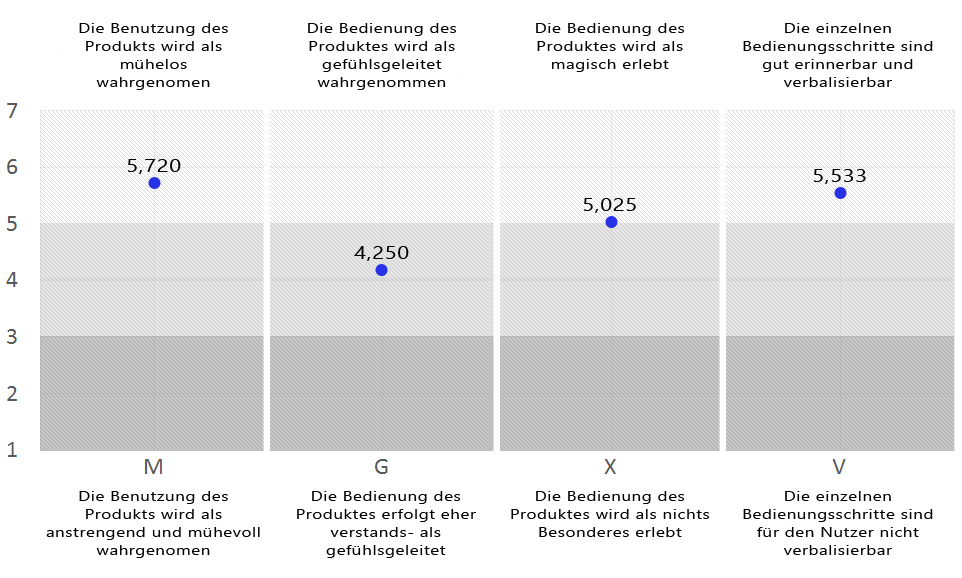
\includegraphics[width=1\textwidth]{img/INTUI_Grafik.jpg}
	\caption{Mittelwerte der 4 Komponenten des INTUI Fragebogens}
	\label{fig:INTUI}
\end{figure}
Der extremste Wert ist mit 5,72 bei der Mühelosigkeit. Das deutet auf eine gute Usability unseres Prototypen hin. Beim Bauchgefühl zeigt der Wert eine minimale Tendenz zu einer gefühlsgeleitenden Interaktion hin. Der Wert des Magischen Erlebens mit 5,025 deutet  auf eine außergewöhnliche Interaktion hin. Die Abfolge unserer Bedienschritt schien unseren Probanden als einleuchtend, zumindest befindet sich der Wert der Verbalisierungsfähigkeit mit 5,533 im oberen Bereich.
\subsection{Ergebnisse des Modells}
Um unsere vorhergesagten Zeiten mit den beobachteten Zeiten vergleichen zu können berechnen wir mit dem Root Mean Square Error (RMSE). Er wird wie folgt berechnet, wobei r unsere beobachteten Zeiten pro Proband (residuals) sind und p die vorhergesagten Zeiten.
\[
RMSE = \sqrt{\frac{1}{n}\sum_{i=1}^{n}(r_i - p_i)^2}
\]
Der RMSE gibt uns an wie viele Sekunden die beobachteten Zeiten durchschnittlich von unserer Vorhersage abweichen. Uns interessiert der prozentuale Fehler, also wird der RMSE noch durch unsere vorhergesagte Zeit geteilt. Wir verwenden eine logarithmische Skala, um die vorhergesagten Zeiten unseres Modells mit den beobachteten Zeiten aus der Evaluation darzustellen, da der Fehler proportional zur Dauer sein soll \citep{Card_1980} und \citep{schneegass_2009}. 

Die \fref{fig:predictedVsObserveredData} zeigt, dass sich unsere vorhergesagten Zeiten sehr gut mit den beobachteten Zeiten decken. 
\begin{figure}
	\centering
		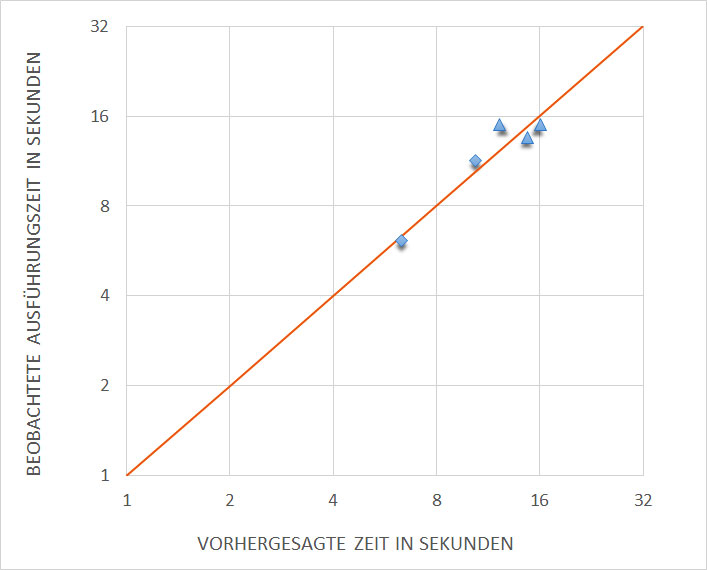
\includegraphics[width=1\textwidth]{img/predictedVsObserveredData.jpg}
	\caption[Übersicht der 5 Aufgaben im Vergleich zu den vorhergesagten und beobachteten Zeiten]{Übersicht der 5 Aufgaben im Vergleich zu den vorhergesagten und beobachteten Zeiten. Die Rauten sind Aufgaben mit nur einem Moduswechsel im Stil der ersten Studie. Die Dreiecke sind die Anwendungsbeispiele mit 2 und 4 Moduswechseln.}
	\label{fig:predictedVsObserveredData}
\end{figure}

Der Durchschnittliche RMSE der 5 Anwendungsbeispiele beträgt 14,746\%, was deutlich geringer ist als die maximale Erwartung von 20-30\% \citep{Card_1980} und generell ganz gut im Bereich von 5\% -20\% liegt \citep{Luo_2005}, \citep{Teo:2006}. Da unser Modell nicht ganz so feingranulare Unterscheidungen macht wie beim KLM und deren Erweiterungen war auch ein größerer Vorhersagefehler zu erwarten. Deshalb ist der durchschnittliche Vorhersagefehler von 14,746\% eine ziemlich gute Annäherung der multimodalen Interaktionszeit. 

In der \fref{tab:PredictedVsObserved} können die vorhergesagten Zeiten, der beobachteten Durchschnittszeiten, der RMSE in Sekunden und prozentual, sowie der durchschnittlichen Belastung des NASA TLX entnommen werden. 
\begin{table}[ht]
  \centering
		\begin{tabular}{|l|l|l|l|l|l|}
				\hline
				Aufgabe			& vorhergesagte 	& durchschnittliche 	& RMSE	& RMSE 		& Beanspruchung\\
				Modi (Wechsel)	& Zeit (s) 				& Zeit (s)						& (s)		& (\%) 		& NASA TLX 	 \\
				\hline
				Lüftung 			& 6,132						& 6,326 (+0,194)								& 0,864	&	14,098	&	25,600\\
				S,T (1)				&& 						&	&		&	\\
				\hline
				Medien Sound	& 11,36						&	10,413 (-0,947)							& 1,614 &	14,202	&	29,700\\
				S,G (1)				&& 						&	&		&	\\
				\hline
				Medien				& 15,014 					&	16,016 (+1,002)							& 1,860	&	12,389	&	33,100\\	
				G,S,T (2)			&& 						&	&		&	\\
				\hline
				Navi POI			& 13,605					& 14,682 (+1,077)							& 1,685	& 12,385	& 32,067\\
				G,S,T (2)			&& 						&	&		&	\\
				\hline
				Navi Nummer		& 15,035					& 12,215	(-2,82)						& 3,105 & 20,654	& 37,533\\		
				T,S (4)				&& 						&	&		&	\\
				\hline	
			\end{tabular}
	\caption[Vorhergesagte Werte im Vergleich zu beobachteten Werten]{Vorhergesagte Werte im Vergleich zu beobachteten Werten, deren RMSE in Sekunden und prozentual, sowie die durchschnittliche Beanspruchung des NASA TLX (Skala von 0-100)}
	\label{tab:PredictedVsObserved}
\end{table}

Unser Modell scheint auch für Interaktionen mit mehr als einem Moduswechsel anwendbar zu sein. Gerade die Vorhersage der Anwendungsbeispiele Medien und Navi POI mit je 3 verschiedenen Modalitäten und somit 2 Modalitätswechsel ergeben die besten Ergebnisse mit einer Fehlerabweichung von nur 12,39\%. 

Die kompletten Ergebnisse aller 10 Probanden dieser beiden Anwendungsbeispiele sind in \fref{fig:Medien_Times} und \fref{fig:Navi_POI_Times} zu sehen. 

Bei dem Anwendungsbeispiel Medien liegt die Durchschnittszeit der Probanden über der vorhergesagten Zeit. Ein Grund dafür kann sein, dass für die Erhebung der Aktion Inkr. (d) eine Verschiebung von 50\% auf das Interval 75-85\% gemessen wurde. In dem Evaluationsbeispiel sollte die Lautstärke von 20\% auf das Interval von 75-85\% gestellt werden. Da hier die Spanne größer ist, könnte dieser Teil etwas länger gedauert haben. 

Auch beim Anwendungsbeispiel Navi POI lag die vorhergesagte Zeit unter dem Durchschnitt. 
\begin{figure}
			\centering
			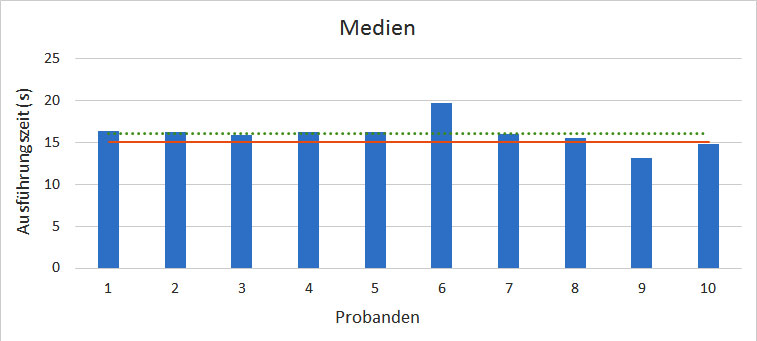
\includegraphics[width=1\textwidth]{img/Medien_Times.jpg}
			\caption[Zeiten der Probanden für das Anwendungsbeispiel Medien.]{Zeiten der Probanden für das Anwendungsbeispiel Medien. Enthält Modalitäten Geste, Sprache und Touch. Die rote durchgehende Linie stellt die vorhergesagte Zeit dar, die grüne gepunktete die Durchschnittszeit aller Probanden.}
			\label{fig:Medien_Times}
\end{figure}
\begin{figure}
			\centering
			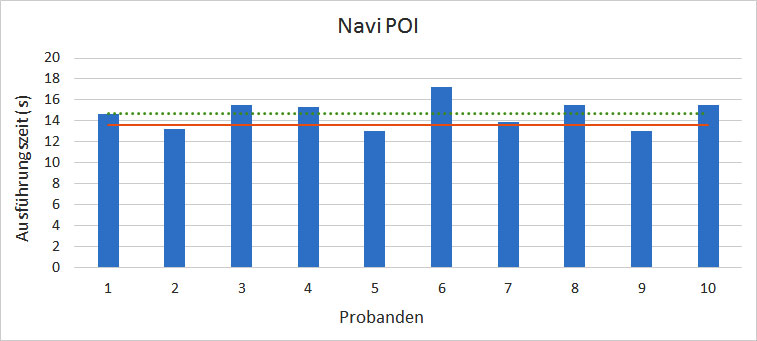
\includegraphics[width=1\textwidth]{img/Navi_POI_Times.jpg}
			\caption[Zeiten der Probanden für das Anwendungsbeispiel Navigation zu POI.]{Zeiten der Probanden für das Anwendungsbeispiel Navigation zu POI. Enthält Modalitäten Geste, Sprache und Touch. Die rote durchgehende Linie stellt die vorhergesagte Zeit dar, die grüne gepunktete die Durchschnittszeit aller Probanden.}
			\label{fig:Navi_POI_Times}		
\end{figure}

Die Anwendungsbeispiele Lüftung und Medien Sound waren fast identisch zu Beispielen aus der ersten Studie. Die hatten beide nur einen Moduswechsel. Beim Anwendungsbeispiel Lüftung liegt unsere Vorhersage unter dem Durchschnitt. Das Anwedungsbeispiel Medien Sound liegt allerdings unsere Vorhersage über dem Durchschnitt. 
Das ist eventuell der Tatsache zu schulden, dass die Probanden der Evaluationsstudie insgesamt besser mit der Slidegeste für die Einstellung des Lautstärkesliders zurecht kamen. 
Die kompletten Ergebnisse aller 10 Probanden dieser beiden Anwendungsbeispiele sind in den \ref{fig:Luft_Times} und \ref{fig:MedienS_Times} zu entnehmen. 
\begin{figure}
			\centering
			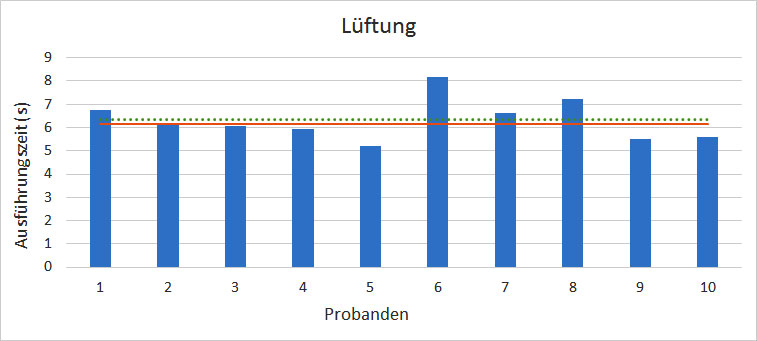
\includegraphics[width=1\textwidth]{img/Luft_Times.jpg}
			\caption[Zeiten der Probanden für das Anwendungsbeispiel Lüftung.]{Zeiten der Probanden für das Anwendungsbeispiel Lüftung. Enthält Modalitäten Sprache und Touch. Die rote durchgehende Linie stellt die vorhergesagte Zeit dar, die grüne gepunktete die Durchschnittszeit aller Probanden.}
			\label{fig:Luft_Times}
\end{figure}
\begin{figure}
			\centering
			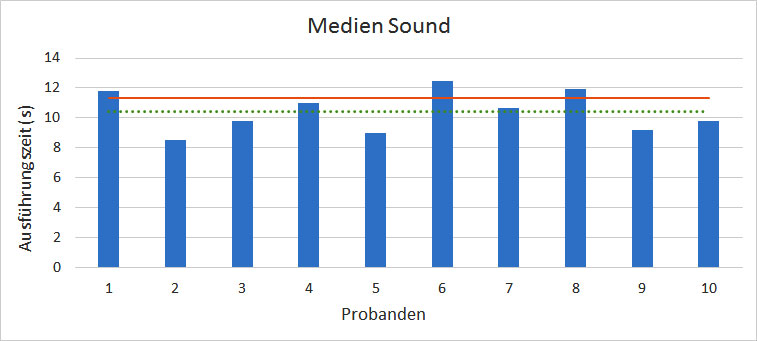
\includegraphics[width=1\textwidth]{img/Medien_S_Times.jpg}
			\caption[Zeiten der Probanden für das Anwendungsbeispiel Medien Sound.]{Zeiten der Probanden für das Anwendungsbeispiel Medien Sound. Enthält Modalitäten Sprache und Geste. Die rote durchgehende Linie stellt die vorhergesagte Zeit dar, die grüne gepunktete die Durchschnittszeit aller Probanden.}
			\label{fig:MedienS_Times}		
\end{figure}

Das Anwendungsbeispiel Navi schnitt am schlechtesten ab mit einem prozentualen RMSE von 20,654\%. Mit zwei verschiedenen Modalitäten und vier Moduswechseln ist dies das aufwändigste Beispiel. Für die Aktivierung der Inputfelder verwendeten wir in unserem Modell zur Vorhersage die Zeit den ersten Buchstaben zu drücken. Im Beispiel ist die Touchfläche allerdings deutlich größer als die Touchfläche der Buchstaben aus unserer ersten Studie. Nach Fitts` Law \citep{fitts1954information}, \citep{sasangohar2009evaluation}
beeinflusst die Größe der Touchfläche W die Interaktionszeit positiv. Es erschien es uns besser die Interaktionszeit zu überschätzen, als zu unterschätzen. Es lässt sich in diesem Beispiel gut erkennen, das unsere Vorhersage für alle Probanden zu groß waren siehe \fref{fig:Navi_Times}.
\begin{figure}
	\centering
		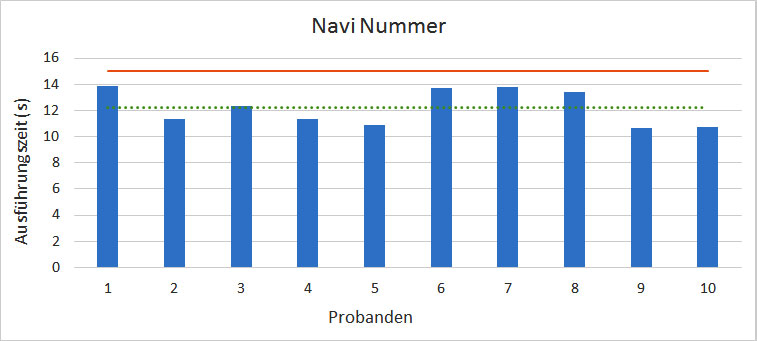
\includegraphics[width=1\textwidth]{img/Navi_Times.jpg}
	\caption[Zeiten der Probanden für das Anwendungsbeispiel Navigation.]{Zeiten der Probanden für das Anwendungsbeispiel Navigation. Enthält Modalitäten Touch, Sprache, Touch, Sprache und Touch. Die rote durchgehende Linie stellt die vorhergesagte Zeit dar, die grüne gepunktete die Durchschnittszeit aller Probanden.}
	\label{fig:Navi_Times}
\end{figure}
\section[Diskussion]{Diskussion}
Die Evaluierung unseres multimodalen Modells soll nun mit Hinblick auf die Ergebnisse diskutiert und mit Ergebnissen aus anderen Arbeiten verglichen werden. Des Weiteren gehen wir auf qualitative Erkenntnisse ein, die sich aus beiden Studien durch Kommentare und Beobachtungen ergeben haben.

\subsection[Modell]{Multimodales Modell}
Die fünf evaluierten Anwendungsbeispiele ließen sich mit unserem Modell mit einem durchschnittlichen RMSE von 14,746\% vorhersagen. Dieser durchschnittliche RMSE befindet sich sowohl im Bereich von 20-30\% den \citet{Card_1980} als maximalen Fehler empfiehlt, als auch im Bereich von 5-20\% \citep{Luo_2005}, \citep{Teo:2006}. \citet{Card_1980}, \citet{Luo_2005} und \citet{Teo:2006} bewerten allerdings ein Keystroke-Level-Modell oder deren Erweiterung auf Operatorebene. Davon ausgehend, dass unser Modell wesentlich grobgranularer aufgebaut ist als das Keystroke-Level-Modell, stellt sich unser Modell zur Vorhersage von multimodalen Interaktionen als vielversprechend heraus. 

\citet{Teo:2006} erklärt, dass es zwei Nachteile bei der Verwendung der gesamten Aufgabendauer gibt. 
Zum einen inkorrekte Messungen und falsch gesetzte Operatoren. 
In unserem Modell haben wir verschiedene Aktionen je nach Modalität und deren Wechselkosten modelliert. 
Eine Aktion enthält allerdings, anders als bei den bisherigen Keystroke-Level Modellen auch mehrere Operatoren. 
Dies macht unser Modell etwas gröber, allerdings ist die Platzierung der Aktionen einfacher. 
Nimmt ein Nutzer die Hand zum Beispiel einmal mehr zurück zum Lenkrad, ist dies kein Fehler, sondern hängt von der Situation ab. 
Diese Unterschiede in der Ausführung der Aktionen steckt in unseren Zeiten mit drinnen. 
Deshalb halten wir die gesamte Dauer der Interaktion für ein geeignetes Maß für den Vergleich. 

Die subjektive Bewertung der Nutzer durch den NASA TLX Ihrer Beanspruchung während der multimodalen Interaktion lag zwischen 25,6 und 37,533 auf einer Skala von 0-100. Den durchschnittlichen Beanspruchungswert von 25,6 hatte das Anwendungsbeispiel Lüftung mit den Modalitäten Sprache und Touch mit einem Moduswechsel. Es lässt sich erkennen, dass die Beanspruchung mit der vorhergesagten Interaktionsdauer zunahm bis zum Wert von 37,533 im Anwendungsbeispiel Navi Nummer. Dieses Anwenungsbeispiel stellte sich mit insgesamt 4 Moduswechseln der Modalitäten Touch und Sprache als das mit der größten Beanspruchung heraus. (Paper mit vergleichbaren Ergebnissen). 

Diese Beanspruchungswerte scheinen in Ordnung zu sein, denn 9 von 10 Teilnehmern können sich eine multimodale Interaktion im Stile unserer Evaluationsstudie während dem Fahren vorstellen. Die intuitive Bedienung, sowie dem Vorteil sich je nach Situation die passende Modalität frei wählen zu können kommt bei den Nutzern gut an. Jedoch bleibt in diesem Feld der multimodalen Interaktion noch viel zu forschen und entwickeln bis die Erwartungen und Vorteile vollends ausgeschöpft werden können.

Beispielsweise haben wir in unserer Evaluation nicht alle Aktionen mit allen Modalitäten evaluiert. Mit 1,5 Stunden dauerte die erste Studie sehr lange und es konnte beobachtet werden, dass die Konzentration mit der Zeit etwas nach ließ. Die Evaluationsstudie wollten wir dementsprechend kürzer gestalten. 

Außerdem haben wir uns speziell Anwendungsbeispiele für die Evaluationsstudie herausgesucht, die uns möglichst realistisch in der Anwendung erschienen. Die Bewertung der Nutzer auf die Eignung der Interaktionen und wie gut sie Ihnen gefallen hat schnitt ganz gut. Das lässt darauf hindeuten, dass unsere Wahl zutreffend war, siehe \fref{fig:Smiley_Eignung_Gefallen}.
Die Texteingabe per Touch wurde nicht evaluiert, da die Spracheignung deutlich besser eingeschätzt wurde. Ebenso die Aktion Inkr. (d) und Inkr. (s) wurde für die Gesteninteraktion nicht evaluiert. 

Die beliebtesten Moduskombinationen der 22 Nutzer aus der ersten Studie waren die unimodale Variante mit Sprache. Am zweit beliebtesten war die Kombination von Touch und Sprache. Die dritt beliebteste Variante war die Kombination von Geste und Sprache. 

Das Design unseres Prototypen wurde Anhand der im Workshop (Connected Minds) gewonnenen Informationen über Interaktionen im Auto modelliert. Wir mussten uns auf bestimmte Gesten einigen, die uns am sinnvollsten erschienen für unsere Aktionen erschienen. Es gibt jedoch andere Varianten, die ebenfalls als Aktionen in Frage kommen. Zum Beispiel die kreisförmige Geste mit dem Zeigefinger nach links oder rechts, um die Lautstärke zu verringern oder zu erhöhen. Eine Geste dieser Art ist bereits im BMW 7 Series eingebaut. Die Implementierung mit der Leap Motion dieser Geste war mit der neuen Version von Unity nicht so einfach umsetzbar, weshalb wir uns dort eine andere Variante überlegten.

Ein weiterer Mangel unseres Modell sind, wie schon erwähnt, die fehlenden haptischen Bedienelemente. Diese sind natürlich ein wichtiger Bestandteil und sollte als weitere Modalität in unser Modell miteinbezogen werden. 

Bei der Aktion Inkr. (d) wurde in der ersten Studie zur Erhebung der Interaktionszeiten lediglich der Slider von 50\% auf 75-85\% verstellt. Für unsere grobe Betrachtung erschien uns diese Einstellung als ausreichend zur Bestimmung dieser Interaktionszeit. Da in dem Anwendungsbeispiel der Evaluation jedoch die Zeiten für eine Verstellung von 20 auf 75-85\% länger dauerte, sollte diese Aktion eventuell genauer untersucht werden. 

\subsection[Qualitative Erkenntnisse]{Qualitative Erkenntnisse}
Während beider Studien zur Bedienung eines multimodalen Interface im Auto ist aufgefallen, dass der Bereich von Gesteninteraktionen sehr individuell von der Sitzeinstellung und Armlänge abhängt. Am ergonomisch geeignetsten hatten es die Nutzer, die ihren Arm an der Armlehne ablegen konnten und sich trotzdem mit der Hand im gewünschten Interaktionsbereich befanden. 

Für zukünftige Gestensteuerung im Auto sollte das berücksichtigt werden, um verkrampfte und unnatürliche Bewegungen zu reduzieren. Zum Beispiel könnte durch eine verstellbare Armlehne, sowie einen anpassbaren Interaktionsbereich zur Gestenerkennung die optimale Einstellung erreicht werden. Das ermöglicht nicht nur eine bequemere Gesteninteraktion, sondern reduziert auch mögliche Erkennungsfehler von Gesten, was wiederum zu einer besseren User Experience führt.

Der Touchbereich war ebenfalls für manche Nutzer nur gut zu Erreichen, indem sie sich etwas vor lehnten. Sie  wurden angewiesen sich vor der Studie den Sitz so einzustellen als würden sie fahren, doch trotz diesen Vorkehrungen war der Touchdisplay nicht für alle optimal positioniert. Auch in der Touchbedienung gibt es noch Potenzial zur Verbesserung. Die Erreichbarkeit des Touchbereichs sollte weiter vorne gelegen sein, als bei Informationssystemen im Auto ohne Touchdisplays.

\chapter{Zusammenfassung und Ausblick}\label{cha:Zusamenfassung}
Ausgehen von den vergangenen und aktuellen Forschungen in Bereichen der Informationssysteme in Fahrzeugen, multimodalen Interaktionen und Modellen zur Bestimmung von Bedienzeiten, wurde in dieser Arbeit ein multimodales Modell vorgestellt, mit deren Hilfe multimodale Interaktionszeiten abgeschätzt und Vergleiche zwischen Kombinationen aus Modalitäten getroffen werden können.

Motiviert wurden wir durch die Vorteile verschiedener Modalitäten und die damit verbundene Möglichkeit, den Nutzer zu entlasten und ihn somit weniger von der Fahraufgabe abzulenken.
Der Fahrer kann selbst entscheiden, in welchen Situationen, welche Modalität für den jeweiligen Schritt am geeignetsten und ungefährlichsten ist, was auch laut \citet{Muller_2011} einen wesentlichen Vorteil in Autos darstellt.

Im Rahmen dieser Arbeit sollte unter anderem erforscht werden, wie multimodale Interaktionen im Fahrzeug aussehen, in welche Aktionen sich diese gliedern lassen und welche Umsetzungsmöglichkeiten sich für die Modalitäten von Haptik, Touch, Geste und Sprache anbieten.
In einem Workshop wurden dazu diverse Anwendungsbeispiele in vereinfachte Aktionen gegliedert und Umsetzungsmöglichkeiten dieser gesammelt.
Auf dieser Grundlage wurde ein Konzept für ein multimodales Modell entworfen und in einem multimodalen Prototypen umgesetzt, der mit Touch-, Gesten- und Spracheingabe bedient werden kann.

Die Basis des implementierten Prototyp bildeten dabei ein Surface zur Erkennung von Touch-Eingaben, ein Leap Motion Controller, um die  Gestenerkennung zu ermöglichen und das Abgreifen definierter Wörtern mit Hilfe der Windows integrierten Spracherkennung.  
Diese wurden in einem 6er Gran Coupé angebracht, um den Interaktionsraum realistisch abzubilden. 

Der Touchdisplay wurde vor das ursprüngliche Display angebracht und der Leap Motion Controller befand sich zwischen Gangschaltung und Dashboard. 
Der Interaktionsbereich für Gesten befand sich in dem Dreiecks-Bereich von Lenkrad, Rückspiegel und Gangschaltung, der von \citet{Riener:2013:SIG} als häufigsten Interaktionsbereich identifiziert wurde.
Für die Benutzerstudie wurden in vier Anwendungsbeispielen alle Kombinationen der Modalitäten Touch, Geste und Sprache mit einem Modalitätswechsel von jedem der 22 Probanden in zwei Messdurchgängen gemessen. 
Um Lerneffekte auszugleichen wurden die Kombinationen permutiert.

Aus dieser Studie konnten wir verschiedene Aktionszeiten für jede Modalität ermitteln und unser multimodales Modell daraus ableiten, das unimodale Aktionszeiten und deren Wechselkosten abbildet. 
Zusätzlich wurde die Eignung und Gefallen der Kombinationen abgefragt, sowie die Eignung der Modalitäten für die verschiedenen Screentypen.

Um das multimodale Modell zu Validieren wurde in einer zweiten Benutzerstudie, der Prototyp für neue Anwendungsbeispiele angepasst, die bis zu vier Modalitätswechsel enthalten.
Die Gesamtdauer der Anwendungsbeispiele wurde mit den, aus dem Modell vorhergesagten, Interaktionszeiten verglichen. 
Mit einem durchschnittlichen Vorhersagefehler von 14,746\% lagen unsere Ergebnisse in den empfohlenen Bereichen von 5-30\% (siehe \citep{Card_1980, Luo_2005,Teo:2006}. 

Mit der Entwicklung unseres Modells zur Vorhersage von multimodalen Interaktionszeiten ist es uns gelungen Designern die Möglichkeit zu geben, bereits in einem frühem Stadium der Entwicklungsphase multimodale Interaktionen einzuschätzen und zu vergleichen. 
Damit können in geeigneter Weise die besten potenziellen Kombinationen unterstützt werden, um dem Fahrer auch die besten Möglichkeiten in verständlicher Weise anzuzeigen. 
Damit soll natürlich auch die visuelle und mentale Beanspruchung für den Fahrer so gering wie möglich gehalten werden. 

Ob eine Variante besonders gut oder schlecht ist hängt natürlich von der Situation ab, deshalb wäre ein seriell redundantes multimodales IVIS am besten, um in jedem Schritt den Fahrer selbst die beste Modalität wählen zu lassen. 
Die Eingabe eines Zieles per Touch ist zum Beispiel im stehenden Auto eine gute Variante, die jedoch während der Fahrt den Fahrer durch die längere Interaktion zu sehr ablenken könnte. 
In diesem Fall stellt die Texteingabe per Sprache eine sehr geeignete Alternative dafür.

Unter Betrachtung der Übertragbarkeit wurden diverse Optimierungen unseres multimodalen Modells erläutert.
Unser Modell zur Vorhersage von multimodalen Interaktionen im IVIS sollte in Zukunft noch dahingehend weiterentwickelt werden auch haptische Bedienelemente mit Aktionszeiten miteinzubeziehen. 
Des weiteren sollte das Modell auf weitere Gesten erweitert werden. 
Außerdem wäre eine detailliertere Untersuchungen von Sprachbefehle bis hin zur Ermittlung von gesprochenen Sätzen ein wichtiger Schritt, um die Interaktionszeiten für zukünftige multimodale Interfaces besser vorhersagen zu können.

Die Validierung unseres Modell wurde nur für einige Aktionen vorgenommen, da wir die Studiendauer in einem Rahmen von 45 Minuten halten wollten. 
Statt alle Aktionen zu testen, einigten wir uns auf fünf Anwendungsbeispiele, die als realistisch Repräsentation von üblichen Anwendungen erschien.
Dabei wurden unter anderem die Einschätzungen der Probanden zur Eignung von Kombinationen der Modalitäten zur Rate gezogen (siehe \fref{fig:Smiley_Eignung_Gefallen}).
Eine komplette Validierung des multimodalen Modells, sollte jedoch noch vorgenommen werden. 

Aus den zwei Studien konnte beobachtet werde, das beide Bereiche für einige Nutzer zu weit positioniert waren.   
Für eine bessere Bedienbarkeit und zur Reduktion der Fahrerablenkung, sollten die Interaktionsbereiche zur Touch-Eingabe und Geste-Eingabe auf ihre Erreichbarkeit verbessert werden. 

\chapter{Danksagung}\label{cha:Danksagung}

Besonderer Dank geht an meine Betreuer Bastian Pfleging und Florian Roider, die mich während dieser Arbeit mit Rat und Tat unterstützt haben. Mein Dank geht natürlich auch an die insgesamt 32 Teilnehmer der zwei Nutzerstudien. Außerdem möchte ich meinem Mann (Sascha Rothe) für seine mentale Unterstützung und spontane Brainstorming Runden danken. 

Für den Prototypen wurden verschiedene Icon von www.flaticon.com verwendet. 
\begin{itemize}
	\item Daumen, Musik Icon: made by Gregor Cresnar (http://www.flaticon.com/authors/gregor-cresnar).
	\item Touch Icon: made by Freepik (http://www.flaticon.com/authors/freepik).
	\item Navigation Icon: made by Madebyoliver (http://www.flaticon.com/authors/madebyoliver). 
	\item Telefon, Gefahr, Touch, Geste und Sprach Icon: made by Freepik (http://www.flaticon.com/authors/freepik). 
	\item Klima Icon: made by Icon Works (http://www.flaticon.com/authors/icon-works). 
\end{itemize}
Flaticon is licensed by Creative Commons BY 3.0 (http://creativecommons.org/licenses/by/3.0/)

 

\chapter{Verzeichnisse}\label{cha:Verzeichnisse}
\begingroup
\renewcommand{\cleardoublepage}{}
\renewcommand{\clearpage}{}

\addcontentsline{toc}{section}{Literaturverzeichnis}
\bibliographystyle{plainnat}
\bibliography{Masterarbeit}

\endgroup
\addcontentsline{toc}{section}{\listfigurename}
\listoffigures% Abbildungsverzeichnis

\addcontentsline{toc}{section}{\listtablename}
\listoftables% Tabellenverzeichnis


\fancyhead[LE,RO,LO,RE]{} % Keine Kopfzeile mehr oben auf jeder Seite
\chapter{Anhang}\label{cha:Anhang}
\begin{enumerate}
	\item Einverständniserklärung
	\item demografischer Fragebogen
	\item Fragebogen nach der Studie
	\item Studienleitfaden
	\item NASA TLX (deutsche Version)
	\item INTUI
\end{enumerate}
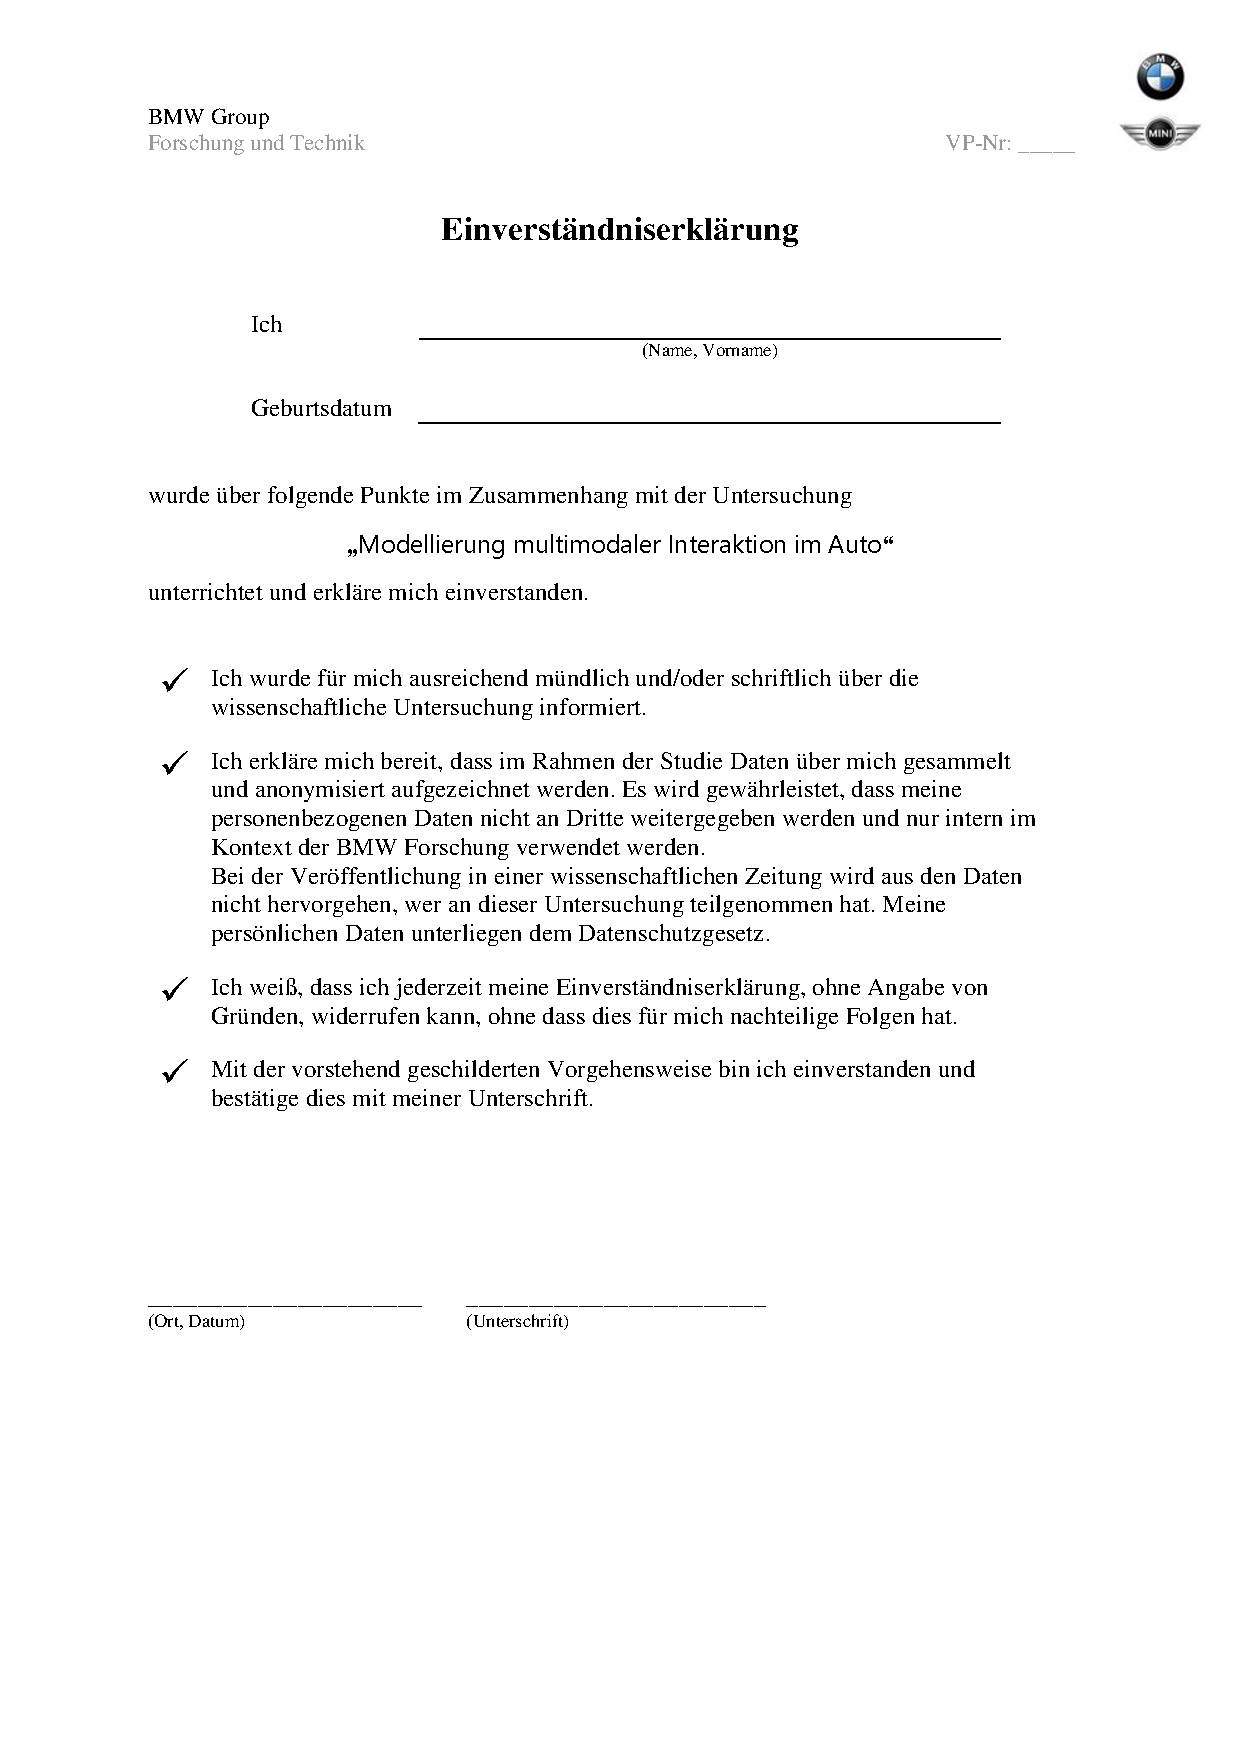
\includepdf[pages=-]{pdf/Einverstaendniserklaerung}
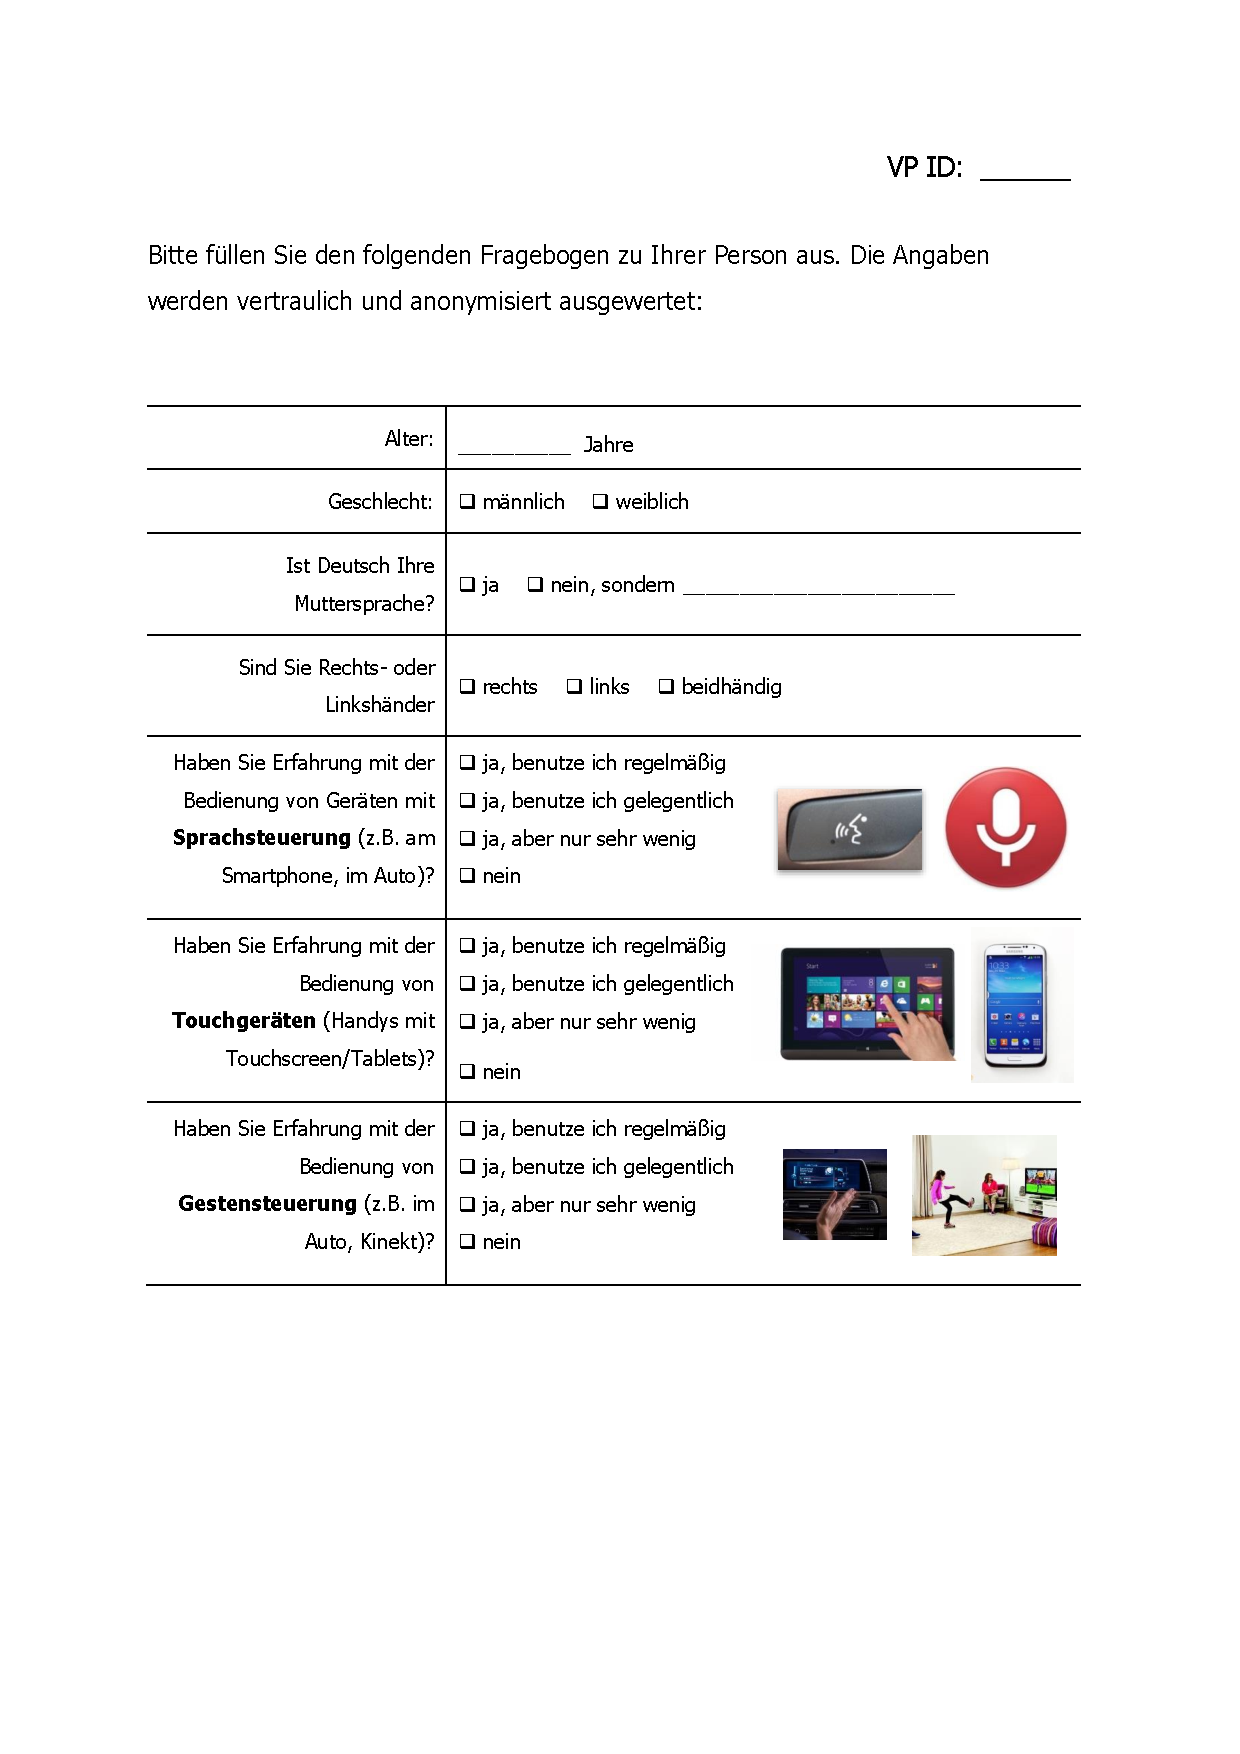
\includepdf[pages=-]{pdf/Fragebogen_dem}
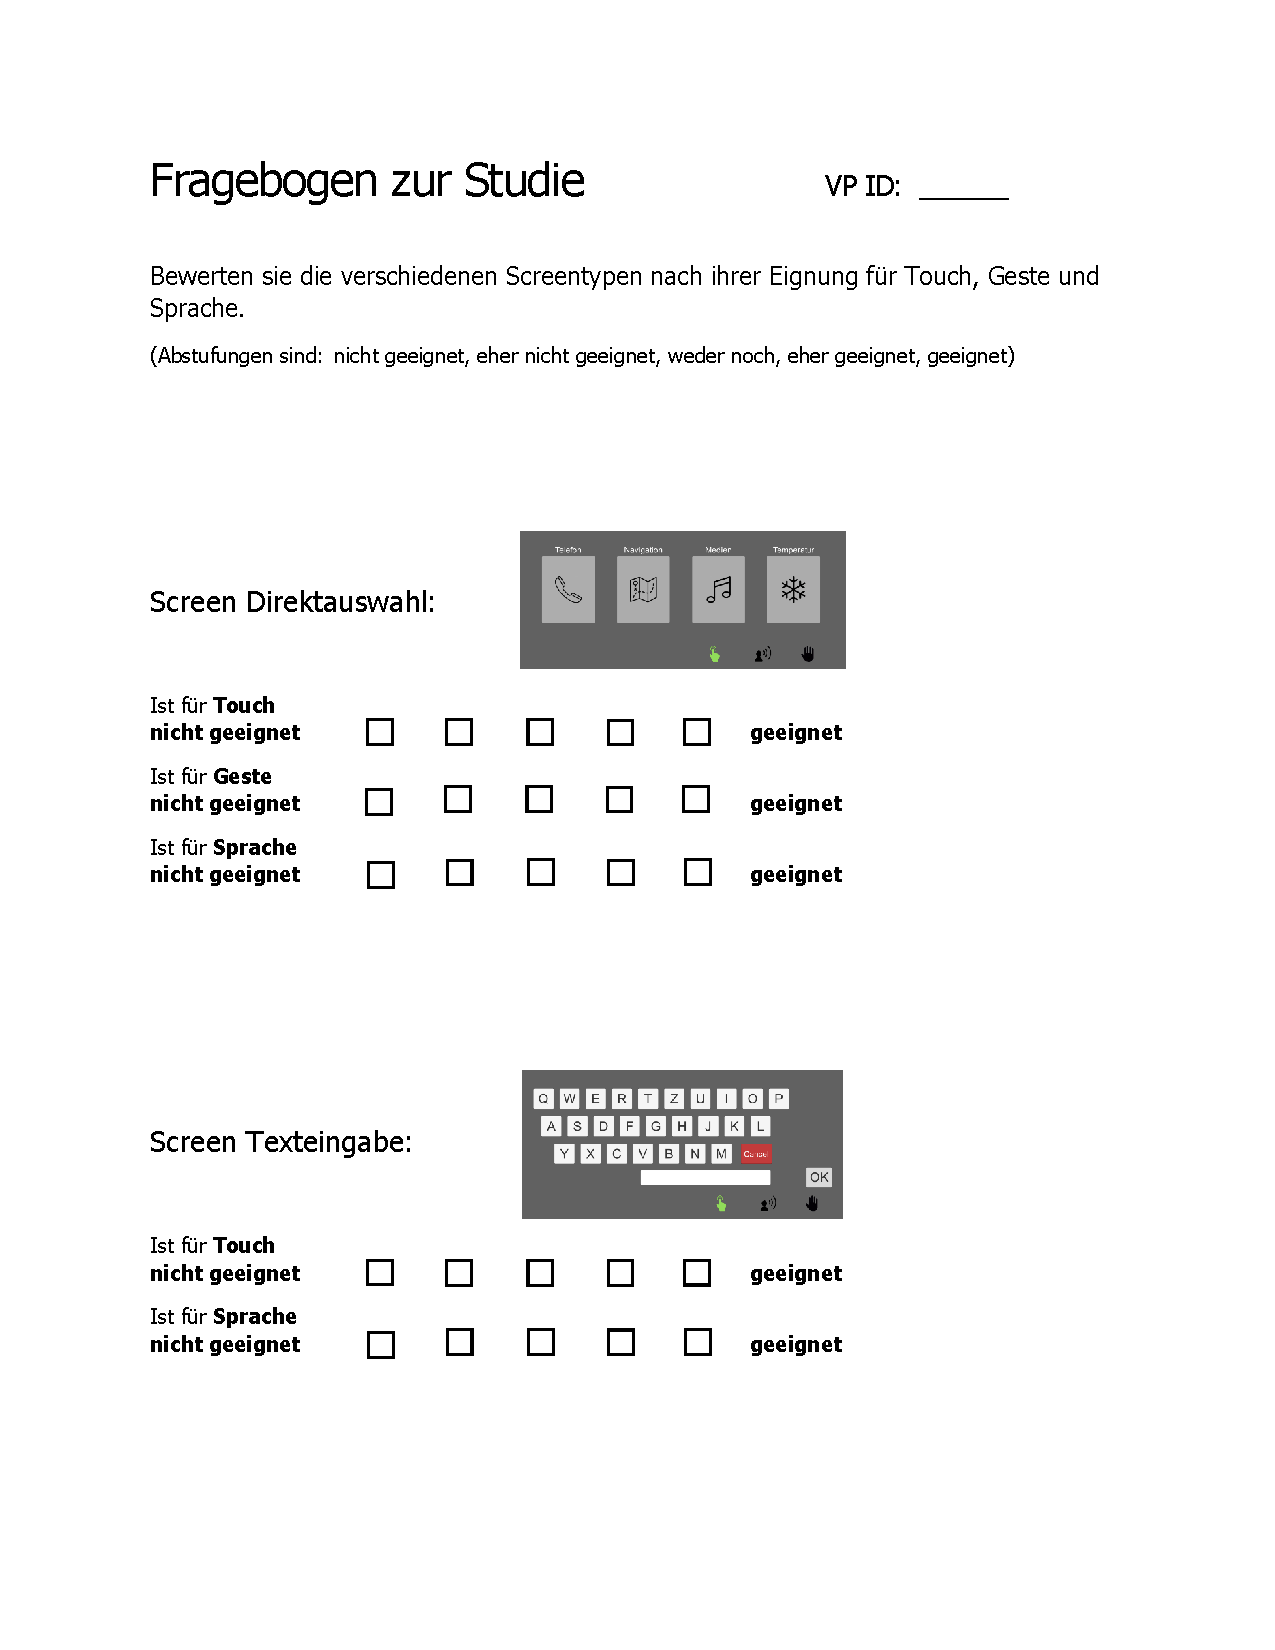
\includepdf[pages=-]{pdf/Fragebogen}
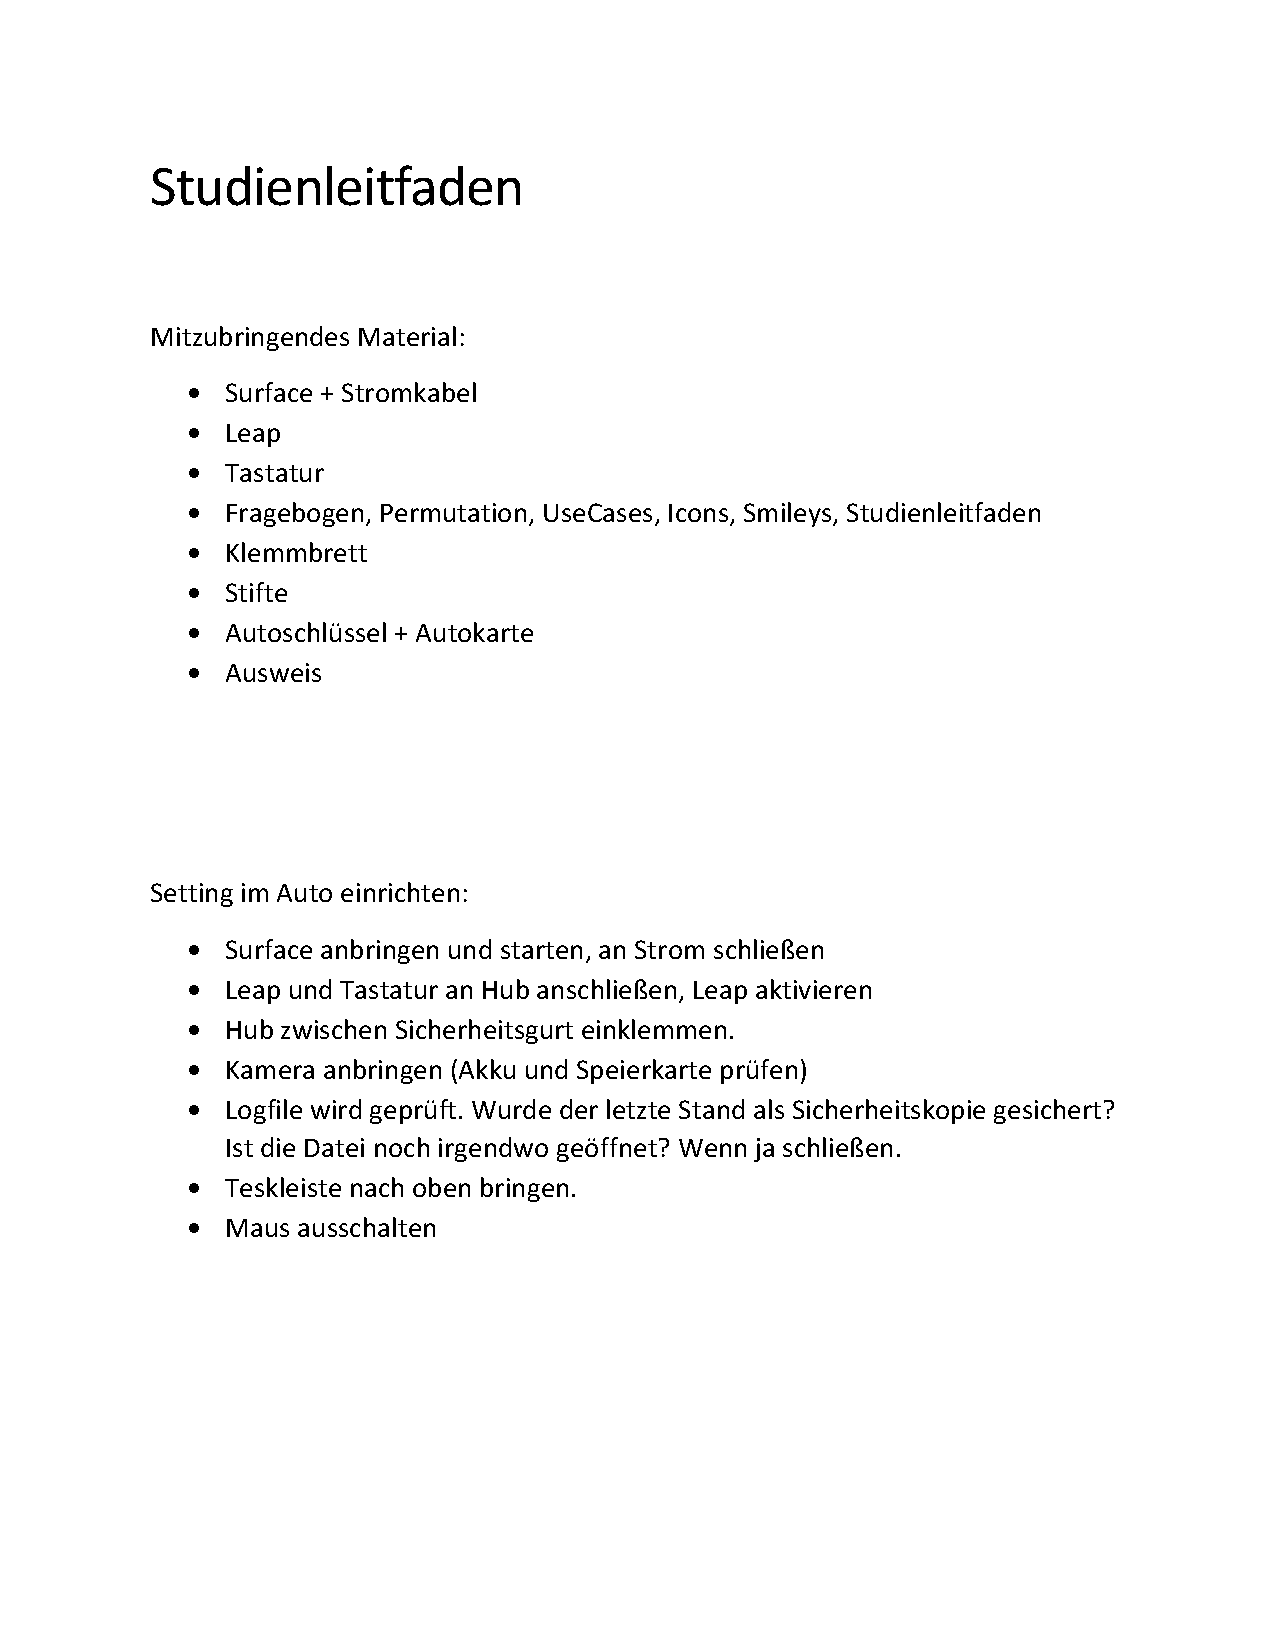
\includepdf[pages=-]{pdf/Studienleitfaden}
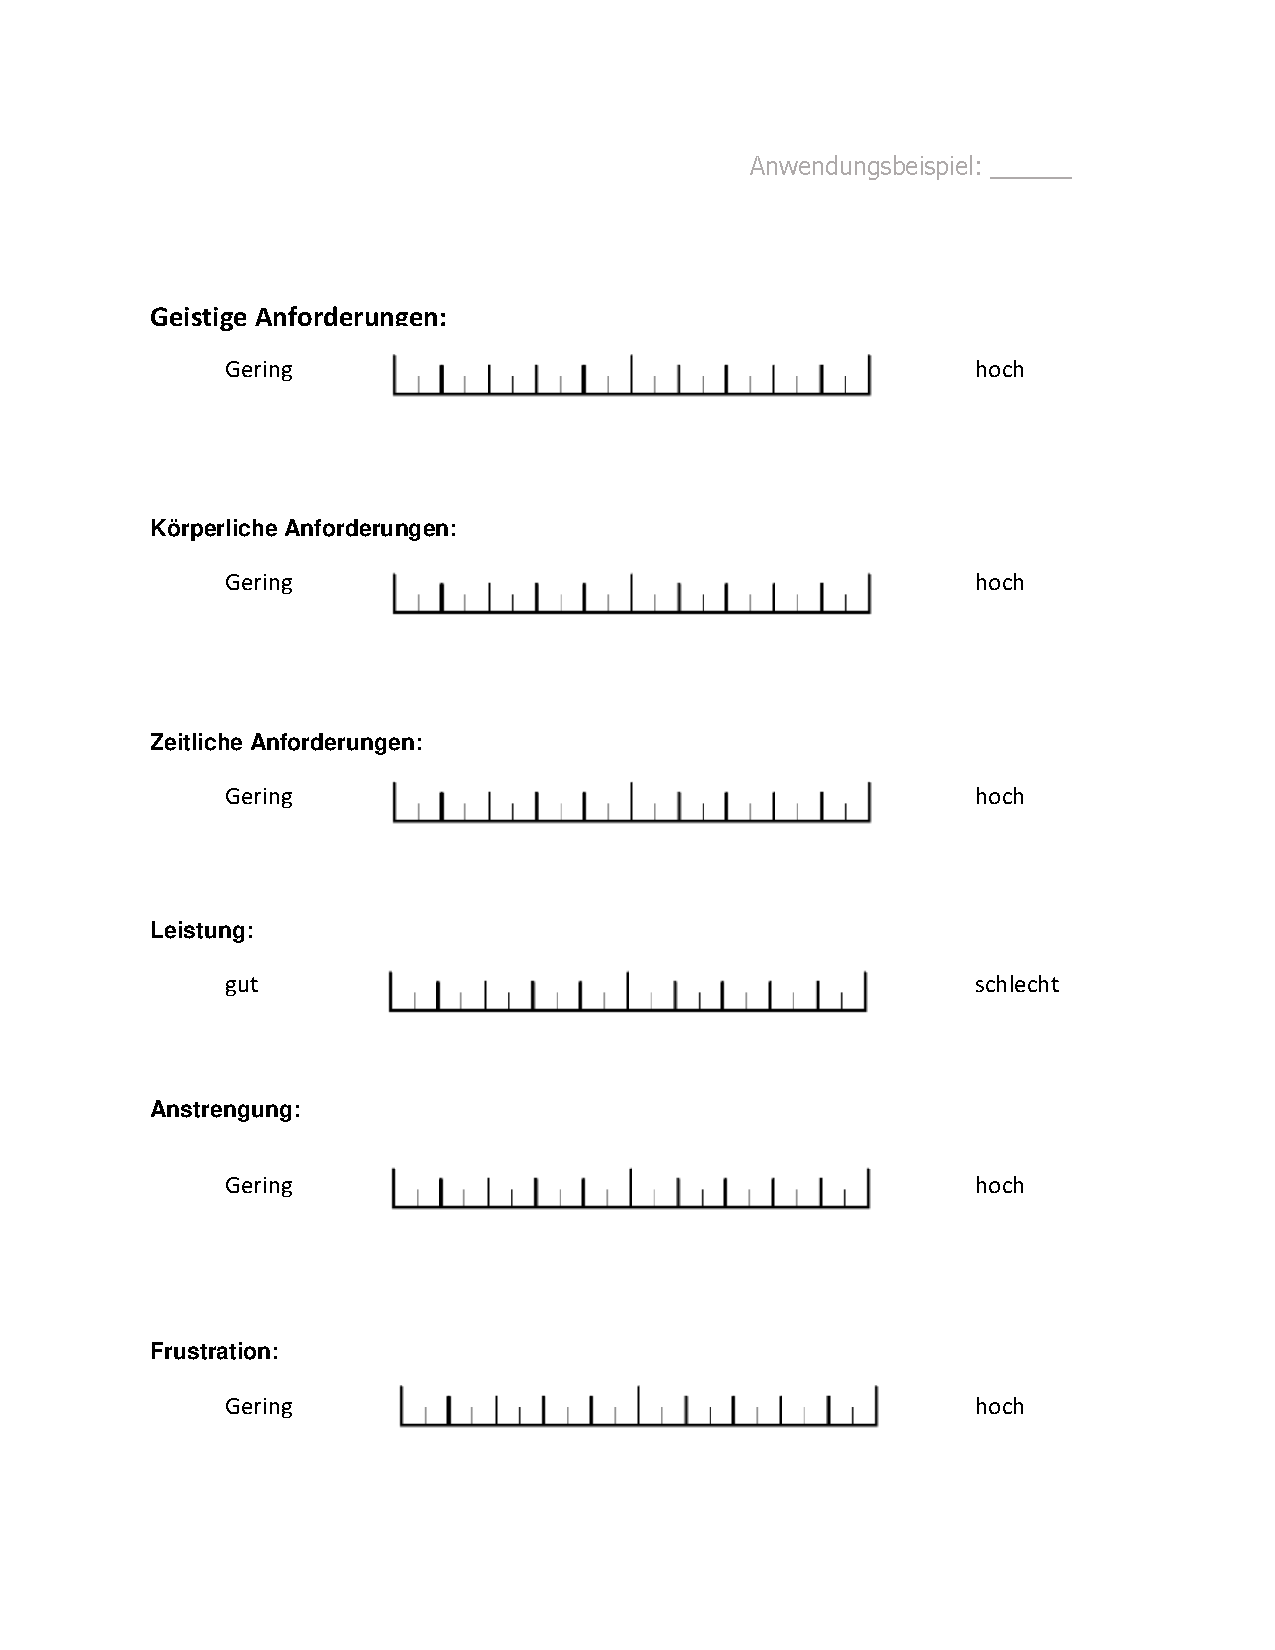
\includepdf[pages=-]{pdf/NASATLX_Teil1}
\includepdf[pages=-]{pdf/INTUI_de}
\includepdf[pages=-]{pdf/Fragebogen_Eval}

\end{document}